\documentclass[a4paper]{book}
\usepackage{a4wide}
\usepackage{makeidx}
\usepackage{fancyhdr}
\usepackage{graphicx}
\usepackage{multicol}
\usepackage{float}
\usepackage{textcomp}
\usepackage{alltt}
\usepackage{doxygen}
\makeindex
\setcounter{tocdepth}{1}
\renewcommand{\footrulewidth}{0.4pt}
\begin{document}
\begin{titlepage}
\vspace*{7cm}
\begin{center}
{\Large SPR Reference Manual}\\
\vspace*{1cm}
{\large Generated by Doxygen 1.4.1}\\
\vspace*{0.5cm}
{\small Mon Oct 2 18:43:17 2006}\\
\end{center}
\end{titlepage}
\clearemptydoublepage
\pagenumbering{roman}
\tableofcontents
\clearemptydoublepage
\pagenumbering{arabic}
\chapter{SPR Directory Hierarchy}
\section{SPR Directories}
This directory hierarchy is sorted roughly, but not completely, alphabetically:\begin{CompactList}
\item \contentsline{section}{src}{\pageref{dir_000000}}{}
\end{CompactList}

\chapter{SPR Namespace Index}
\section{SPR Namespace List}
Here is a list of all namespaces with brief descriptions:\begin{CompactList}
\item\contentsline{section}{{\bf std} }{\pageref{namespacestd}}{}
\end{CompactList}

\chapter{SPR Hierarchical Index}
\section{SPR Class Hierarchy}
This inheritance list is sorted roughly, but not completely, alphabetically:\begin{CompactList}
\item \contentsline{section}{Bracket\-Table$<$ T $>$}{\pageref{classBracketTable}}{}
\item \contentsline{section}{Chain\-Table$<$ T $>$}{\pageref{classChainTable}}{}
\item \contentsline{section}{Chain\-Table$<$ T $>$::NList$<$ T $>$}{\pageref{structChainTable_1_1NList}}{}
\item \contentsline{section}{Cherry\-Table$<$ T $>$}{\pageref{classCherryTable}}{}
\item \contentsline{section}{Crc32$<$ T $>$}{\pageref{classCrc32}}{}
\item \contentsline{section}{CVector$<$ T $>$}{\pageref{classCVector}}{}
\begin{CompactList}
\item \contentsline{section}{Split$<$ T $>$}{\pageref{classSplit}}{}
\end{CompactList}
\item \contentsline{section}{Extract\-Splits\-Forest}{\pageref{classExtractSplitsForest}}{}
\item \contentsline{section}{Extract\-Subtree$<$ T, U $>$}{\pageref{classExtractSubtree}}{}
\item \contentsline{section}{Flag\-Table$<$ T $>$}{\pageref{classFlagTable}}{}
\item \contentsline{section}{Flag\-Table$<$ T $>$::Flag$<$ T $>$}{\pageref{structFlagTable_1_1Flag}}{}
\item \contentsline{section}{Flag\-Table$<$ T $>$::Neighbours$<$ T $>$}{\pageref{structFlagTable_1_1Neighbours}}{}
\item \contentsline{section}{Kernelizor$<$ T $>$}{\pageref{classKernelizor}}{}
\item \contentsline{section}{Split\-PLess$<$ T $>$}{\pageref{structSplitPLess}}{}
\item \contentsline{section}{Split\-Table$<$ T $>$}{\pageref{classSplitTable}}{}
\item \contentsline{section}{Spr\-Helper$<$ T $>$}{\pageref{classSprHelper}}{}
\item \contentsline{section}{SPRSearch$<$ T $>$}{\pageref{classSPRSearch}}{}
\item \contentsline{section}{Spr\-Table$<$ T $>$}{\pageref{classSprTable}}{}
\item \contentsline{section}{Spr\-Table$<$ T $>$::NList$<$ T $>$}{\pageref{structSprTable_1_1NList}}{}
\item \contentsline{section}{Subtree\-Rec$<$ T $>$}{\pageref{structSubtreeRec}}{}
\item \contentsline{section}{Tree\-Cache$<$ T $>$}{\pageref{classTreeCache}}{}
\item \contentsline{section}{Tree\-Cache$<$ T $>$::Node$<$ T $>$}{\pageref{structTreeCache_1_1Node}}{}
\item \contentsline{section}{Tree\-Cache$<$ T $>$::Result$<$ T $>$}{\pageref{structTreeCache_1_1Result}}{}
\item \contentsline{section}{Tree\-Distance$<$ T $>$}{\pageref{classTreeDistance}}{}
\item \contentsline{section}{Tree\-Manager$<$ T $>$}{\pageref{classTreeManager}}{}
\item \contentsline{section}{Tree\-Tok$<$ T $>$}{\pageref{structTreeTok}}{}
\item \contentsline{section}{UPTree$<$ T $>$}{\pageref{structUPTree}}{}
\item \contentsline{section}{Validator$<$ T $>$}{\pageref{classValidator}}{}
\end{CompactList}

\chapter{SPR Class Index}
\section{SPR Class List}
Here are the classes, structs, unions and interfaces with brief descriptions:\begin{CompactList}
\item\contentsline{section}{{\bf Bracket\-Table$<$ T $>$} (The brackettable stores some information from the tree strings for quick lookup: For each bracket, the offeset of its matching bracket is stored )}{\pageref{classBracketTable}}{}
\item\contentsline{section}{{\bf Chain\-Table$<$ T $>$} (Computes and stores the offsets of pendant leaves that are neighbours in a chain )}{\pageref{classChainTable}}{}
\item\contentsline{section}{{\bf Chain\-Table$<$ T $>$::NList$<$ T $>$} (The chain neighbours of a leaf )}{\pageref{structChainTable_1_1NList}}{}
\item\contentsline{section}{{\bf Cherry\-Table$<$ T $>$} (Stores the position of cherry neighbour of each leaf in the tree )}{\pageref{classCherryTable}}{}
\item\contentsline{section}{{\bf Crc32$<$ T $>$} }{\pageref{classCrc32}}{}
\item\contentsline{section}{{\bf CVector$<$ T $>$} (This is a c-style implementation of std::vector )}{\pageref{classCVector}}{}
\item\contentsline{section}{{\bf Extract\-Splits\-Forest} }{\pageref{classExtractSplitsForest}}{}
\item\contentsline{section}{{\bf Extract\-Subtree$<$ T, U $>$} }{\pageref{classExtractSubtree}}{}
\item\contentsline{section}{{\bf Flag\-Table$<$ T $>$} (This class keeps track of a boolean flag for each element of a tree string )}{\pageref{classFlagTable}}{}
\item\contentsline{section}{{\bf Flag\-Table$<$ T $>$::Flag$<$ T $>$} ({\bf Flag}{\rm (p.\,\pageref{structFlagTable_1_1Flag})} can specify if a given node is marked as frozen and/or marked for deletion )}{\pageref{structFlagTable_1_1Flag}}{}
\item\contentsline{section}{{\bf Flag\-Table$<$ T $>$::Neighbours$<$ T $>$} (Offset the next unflagged neighbour to the left and right of a position )}{\pageref{structFlagTable_1_1Neighbours}}{}
\item\contentsline{section}{{\bf Kernelizor$<$ T $>$} (Kernelizes pairs of trees by flagging common subtrees and chains in accordance with Rule 1 and Rule 2 )}{\pageref{classKernelizor}}{}
\item\contentsline{section}{{\bf Split$<$ T $>$} (A split corresponds to the bipartition of the leaf set induced by an internal edge )}{\pageref{classSplit}}{}
\item\contentsline{section}{{\bf Split\-PLess$<$ T $>$} ({\bf Split}{\rm (p.\,\pageref{classSplit})} pointer comparison )}{\pageref{structSplitPLess}}{}
\item\contentsline{section}{{\bf Split\-Table$<$ T $>$} (The split table can load all non-trivial splits of a tree and provide set-like operations with split tables of other trees in order to identify common splits )}{\pageref{classSplitTable}}{}
\item\contentsline{section}{{\bf Spr\-Helper$<$ T $>$} (Provides quick access to subtrees after a retrifurcation )}{\pageref{classSprHelper}}{}
\item\contentsline{section}{{\bf SPRSearch$<$ T $>$} (Breadth first search of SPR-neighbour graph )}{\pageref{classSPRSearch}}{}
\item\contentsline{section}{{\bf Spr\-Table$<$ T $>$} (Stores all possible regraft points for every subtree in a tree )}{\pageref{classSprTable}}{}
\item\contentsline{section}{{\bf Spr\-Table$<$ T $>$::NList$<$ T $>$} (List of valid regraft points )}{\pageref{structSprTable_1_1NList}}{}
\item\contentsline{section}{{\bf Subtree\-Rec$<$ T $>$} (Record corresponding to the information of one subtree )}{\pageref{structSubtreeRec}}{}
\item\contentsline{section}{{\bf Tree\-Cache$<$ T $>$} (Hash table with chaining that stores to references to trees )}{\pageref{classTreeCache}}{}
\item\contentsline{section}{{\bf Tree\-Cache$<$ T $>$::Node$<$ T $>$} (May want to templatize offset? maximum currently iteration hardcoded to 16 ==$>$ maximum distance is 32 os is potentially too small!! TODO: global max os value )}{\pageref{structTreeCache_1_1Node}}{}
\item\contentsline{section}{{\bf Tree\-Cache$<$ T $>$::Result$<$ T $>$} ({\bf Result}{\rm (p.\,\pageref{structTreeCache_1_1Result})} token for returning status of a call to {\bf update()}{\rm (p.\,\pageref{classTreeCache_a4})} )}{\pageref{structTreeCache_1_1Result}}{}
\item\contentsline{section}{{\bf Tree\-Distance$<$ T $>$} (Compute SPR-distance between two unrooted NEWICK trees )}{\pageref{classTreeDistance}}{}
\item\contentsline{section}{{\bf Tree\-Manager$<$ T $>$} (Stores a given number of trees in a contiguous chunk of memory )}{\pageref{classTreeManager}}{}
\item\contentsline{section}{{\bf Tree\-Tok$<$ T $>$} (Token used in the binary tree representation )}{\pageref{structTreeTok}}{}
\item\contentsline{section}{{\bf UPTree$<$ T $>$} (Binary-array representation of an Unrooted Phylogenetic Tree )}{\pageref{structUPTree}}{}
\item\contentsline{section}{{\bf Validator$<$ T $>$} (Validator class is responsible for verifying that a tree is properly formed )}{\pageref{classValidator}}{}
\end{CompactList}

\chapter{SPR File Index}
\section{SPR File List}
Here is a list of all files with brief descriptions:\begin{CompactList}
\item\contentsline{section}{{\bf brackettable.h} }{\pageref{brackettable_8h}}{}
\item\contentsline{section}{{\bf brackettable\_\-impl.h} }{\pageref{brackettable__impl_8h}}{}
\item\contentsline{section}{{\bf chaintable.h} }{\pageref{chaintable_8h}}{}
\item\contentsline{section}{{\bf chaintable\_\-impl.h} }{\pageref{chaintable__impl_8h}}{}
\item\contentsline{section}{{\bf cherrytable.h} }{\pageref{cherrytable_8h}}{}
\item\contentsline{section}{{\bf cherrytable\_\-impl.h} }{\pageref{cherrytable__impl_8h}}{}
\item\contentsline{section}{{\bf constants.cpp} }{\pageref{constants_8cpp}}{}
\item\contentsline{section}{{\bf crc32.h} }{\pageref{crc32_8h}}{}
\item\contentsline{section}{{\bf crc32\_\-impl.h} }{\pageref{crc32__impl_8h}}{}
\item\contentsline{section}{{\bf cvector.h} }{\pageref{cvector_8h}}{}
\item\contentsline{section}{{\bf cvector\_\-impl.h} }{\pageref{cvector__impl_8h}}{}
\item\contentsline{section}{{\bf extractsplitsforest.cpp} }{\pageref{extractsplitsforest_8cpp}}{}
\item\contentsline{section}{{\bf extractsplitsforest.h} }{\pageref{extractsplitsforest_8h}}{}
\item\contentsline{section}{{\bf extractsplitsforest\_\-impl.h} }{\pageref{extractsplitsforest__impl_8h}}{}
\item\contentsline{section}{{\bf extractsubtree.h} }{\pageref{extractsubtree_8h}}{}
\item\contentsline{section}{{\bf extractsubtree\_\-impl.h} }{\pageref{extractsubtree__impl_8h}}{}
\item\contentsline{section}{{\bf flagtable.h} }{\pageref{flagtable_8h}}{}
\item\contentsline{section}{{\bf flagtable\_\-impl.h} }{\pageref{flagtable__impl_8h}}{}
\item\contentsline{section}{{\bf kernelize.cpp} }{\pageref{kernelize_8cpp}}{}
\item\contentsline{section}{{\bf kernelizor.h} }{\pageref{kernelizor_8h}}{}
\item\contentsline{section}{{\bf kernelizor\_\-impl.h} }{\pageref{kernelizor__impl_8h}}{}
\item\contentsline{section}{{\bf randtree.cpp} }{\pageref{randtree_8cpp}}{}
\item\contentsline{section}{{\bf splittable.h} }{\pageref{splittable_8h}}{}
\item\contentsline{section}{{\bf splittable\_\-impl.h} }{\pageref{splittable__impl_8h}}{}
\item\contentsline{section}{{\bf sprdist.cpp} }{\pageref{sprdist_8cpp}}{}
\item\contentsline{section}{{\bf sprhelper.h} }{\pageref{sprhelper_8h}}{}
\item\contentsline{section}{{\bf sprhelper\_\-impl.h} }{\pageref{sprhelper__impl_8h}}{}
\item\contentsline{section}{{\bf sprsearch.h} }{\pageref{sprsearch_8h}}{}
\item\contentsline{section}{{\bf sprsearch\_\-impl.h} }{\pageref{sprsearch__impl_8h}}{}
\item\contentsline{section}{{\bf sprtable.h} }{\pageref{sprtable_8h}}{}
\item\contentsline{section}{{\bf sprtable\_\-impl.h} }{\pageref{sprtable__impl_8h}}{}
\item\contentsline{section}{{\bf treecache.h} }{\pageref{treecache_8h}}{}
\item\contentsline{section}{{\bf treecache\_\-impl.h} }{\pageref{treecache__impl_8h}}{}
\item\contentsline{section}{{\bf treedistance.cpp} }{\pageref{treedistance_8cpp}}{}
\item\contentsline{section}{{\bf treedistance.h} }{\pageref{treedistance_8h}}{}
\item\contentsline{section}{{\bf treemanager.h} }{\pageref{treemanager_8h}}{}
\item\contentsline{section}{{\bf treemanager\_\-impl.h} }{\pageref{treemanager__impl_8h}}{}
\item\contentsline{section}{{\bf treetok.h} }{\pageref{treetok_8h}}{}
\item\contentsline{section}{{\bf treetok\_\-impl.h} }{\pageref{treetok__impl_8h}}{}
\item\contentsline{section}{{\bf uptree.h} }{\pageref{uptree_8h}}{}
\item\contentsline{section}{{\bf uptree\_\-impl.h} }{\pageref{uptree__impl_8h}}{}
\item\contentsline{section}{{\bf validator.h} }{\pageref{validator_8h}}{}
\item\contentsline{section}{{\bf validator\_\-impl.h} }{\pageref{validator__impl_8h}}{}
\end{CompactList}

\chapter{SPR Directory Documentation}
\section{/home/hickey/Code/thesis/spr/src/ Directory Reference}
\label{dir_000000}\index{/home/hickey/Code/thesis/spr/src/ Directory Reference@{/home/hickey/Code/thesis/spr/src/ Directory Reference}}
\subsection*{Files}
\begin{CompactItemize}
\item 
file {\bf brackettable.h}
\item 
file {\bf brackettable\_\-impl.h}
\item 
file {\bf chaintable.h}
\item 
file {\bf chaintable\_\-impl.h}
\item 
file {\bf cherrytable.h}
\item 
file {\bf cherrytable\_\-impl.h}
\item 
file {\bf constants.cpp}
\item 
file {\bf crc32.h}
\item 
file {\bf crc32\_\-impl.h}
\item 
file {\bf cvector.h}
\item 
file {\bf cvector\_\-impl.h}
\item 
file {\bf extractsplitsforest.cpp}
\item 
file {\bf extractsplitsforest.h}
\item 
file {\bf extractsplitsforest\_\-impl.h}
\item 
file {\bf extractsubtree.h}
\item 
file {\bf extractsubtree\_\-impl.h}
\item 
file {\bf flagtable.h}
\item 
file {\bf flagtable\_\-impl.h}
\item 
file {\bf kernelize.cpp}
\item 
file {\bf kernelizor.h}
\item 
file {\bf kernelizor\_\-impl.h}
\item 
file {\bf randtree.cpp}
\item 
file {\bf splittable.h}
\item 
file {\bf splittable\_\-impl.h}
\item 
file {\bf sprdist.cpp}
\item 
file {\bf sprhelper.h}
\item 
file {\bf sprhelper\_\-impl.h}
\item 
file {\bf sprsearch.h}
\item 
file {\bf sprsearch\_\-impl.h}
\item 
file {\bf sprtable.h}
\item 
file {\bf sprtable\_\-impl.h}
\item 
file {\bf treecache.h}
\item 
file {\bf treecache\_\-impl.h}
\item 
file {\bf treedistance.cpp}
\item 
file {\bf treedistance.h}
\item 
file {\bf treemanager.h}
\item 
file {\bf treemanager\_\-impl.h}
\item 
file {\bf treetok.h}
\item 
file {\bf treetok\_\-impl.h}
\item 
file {\bf uptree.h}
\item 
file {\bf uptree\_\-impl.h}
\item 
file {\bf validator.h}
\item 
file {\bf validator\_\-impl.h}
\end{CompactItemize}

\chapter{SPR Namespace Documentation}
\section{std Namespace Reference}
\label{namespacestd}\index{std@{std}}



\chapter{SPR Class Documentation}
\section{Bracket\-Table$<$ T $>$ Class Template Reference}
\label{classBracketTable}\index{BracketTable@{BracketTable}}
The brackettable stores some information from the tree strings for quick lookup: For each bracket, the offeset of its matching bracket is stored.  


{\tt \#include $<$brackettable.h$>$}

\subsection*{Public Member Functions}
\begin{CompactItemize}
\item 
{\bf Bracket\-Table} ()
\item 
{\bf Bracket\-Table} (int)
\item 
{\bf $\sim$Bracket\-Table} ()
\item 
void {\bf resize} (int)
\begin{CompactList}\small\item\em Resize the table if necessary. \item\end{CompactList}\item 
int {\bf get\-Size} () const 
\begin{CompactList}\small\item\em Return size of the table. \item\end{CompactList}\item 
int {\bf load\-Tree} (const {\bf UPTree}$<$ T $>$ \&)
\begin{CompactList}\small\item\em Create a table corresponding to a given tree. \item\end{CompactList}\item 
int {\bf load\-Subtree} (const {\bf UPTree}$<$ T $>$ \&, int, int)
\begin{CompactList}\small\item\em Load a subtree into the table. \item\end{CompactList}\item 
const {\bf Subtree\-Rec}$<$ T $>$ $\ast$ {\bf get\-Table} () const 
\begin{CompactList}\small\item\em Return a const reference to the entire table contents. \item\end{CompactList}\item 
{\bf Subtree\-Rec}$<$ T $>$ \& {\bf operator[$\,$]} (int)
\begin{CompactList}\small\item\em Get a reference to the table record corresponding to a particular offset. \item\end{CompactList}\item 
const {\bf Subtree\-Rec}$<$ T $>$ \& {\bf operator[$\,$]} (int) const 
\begin{CompactList}\small\item\em Get a const reference to the table record corresponding to a particular offset. \item\end{CompactList}\item 
const {\bf Subtree\-Rec}$<$ T $>$ \& {\bf at} (int) const 
\begin{CompactList}\small\item\em Get a const reference to the table record corresponding to a particular offset. \item\end{CompactList}\item 
int {\bf get\-Tri\-Pos} (int) const 
\begin{CompactList}\small\item\em Get the trifurcation number of the subtree containing the token at a specified position. \item\end{CompactList}\item 
void {\bf get\-Tri\-Pos} (int[3]) const 
\begin{CompactList}\small\item\em Get a copy of the start positions of each of the 3 subtrees corresponding to the trifurcation. \item\end{CompactList}\item 
const int $\ast$ {\bf get\-Tri\-Pos} () const 
\begin{CompactList}\small\item\em Get the start positions of each of the 3 subtrees corresponding to the trifurcation. \item\end{CompactList}\end{CompactItemize}
\subsection*{Protected Attributes}
\begin{CompactItemize}
\item 
std::stack$<$ T $>$ {\bf \_\-stack}
\item 
{\bf Subtree\-Rec}$<$ T $>$ $\ast$ {\bf \_\-table}
\begin{CompactList}\small\item\em General purpose stack. I should change T to int. \item\end{CompactList}\item 
int {\bf \_\-tab\-Size}
\begin{CompactList}\small\item\em The actual table structure which is just an array. \item\end{CompactList}\item 
int {\bf \_\-tri\-Pos} [3]
\begin{CompactList}\small\item\em Size of the table. \item\end{CompactList}\end{CompactItemize}


\subsection{Detailed Description}
\subsubsection*{template$<$class T$>$ class Bracket\-Table$<$ T $>$}

The brackettable stores some information from the tree strings for quick lookup: For each bracket, the offeset of its matching bracket is stored. 

For each pair of matching brackets, the position of the corresponding bifurcation as well as the minimum leaf label value contained in each subtree is stored. Finally, the offset of the start position of each trifurcation in the string is stored. 



\subsection{Constructor \& Destructor Documentation}
\index{BracketTable@{Bracket\-Table}!BracketTable@{BracketTable}}
\index{BracketTable@{BracketTable}!BracketTable@{Bracket\-Table}}
\subsubsection{\setlength{\rightskip}{0pt plus 5cm}template$<$class T$>$ {\bf Bracket\-Table}$<$ T $>$::{\bf Bracket\-Table} ()}\label{classBracketTable_a0}


\index{BracketTable@{Bracket\-Table}!BracketTable@{BracketTable}}
\index{BracketTable@{BracketTable}!BracketTable@{Bracket\-Table}}
\subsubsection{\setlength{\rightskip}{0pt plus 5cm}template$<$class T$>$ {\bf Bracket\-Table}$<$ T $>$::{\bf Bracket\-Table} (int {\em size})}\label{classBracketTable_a1}


\begin{Desc}
\item[Parameters:]
\begin{description}
\item[{\em size}]Size of table to create. Note that this is total number of nodes, not number of leaves. \end{description}
\end{Desc}
\index{BracketTable@{Bracket\-Table}!~BracketTable@{$\sim$BracketTable}}
\index{~BracketTable@{$\sim$BracketTable}!BracketTable@{Bracket\-Table}}
\subsubsection{\setlength{\rightskip}{0pt plus 5cm}template$<$class T$>$ {\bf Bracket\-Table}$<$ T $>$::$\sim${\bf Bracket\-Table} ()}\label{classBracketTable_a2}




\subsection{Member Function Documentation}
\index{BracketTable@{Bracket\-Table}!at@{at}}
\index{at@{at}!BracketTable@{Bracket\-Table}}
\subsubsection{\setlength{\rightskip}{0pt plus 5cm}template$<$class T$>$ const {\bf Subtree\-Rec}$<$ T $>$ \& {\bf Bracket\-Table}$<$ T $>$::at (int {\em pos}) const\hspace{0.3cm}{\tt  [inline]}}\label{classBracketTable_a10}


Get a const reference to the table record corresponding to a particular offset. 

Easier to use on pointers than oeprator[]. \begin{Desc}
\item[Parameters:]
\begin{description}
\item[{\em pos}]Position of desired record. \end{description}
\end{Desc}
\index{BracketTable@{Bracket\-Table}!getSize@{getSize}}
\index{getSize@{getSize}!BracketTable@{Bracket\-Table}}
\subsubsection{\setlength{\rightskip}{0pt plus 5cm}template$<$class T$>$ int {\bf Bracket\-Table}$<$ T $>$::get\-Size () const}\label{classBracketTable_a4}


Return size of the table. 

\index{BracketTable@{Bracket\-Table}!getTable@{getTable}}
\index{getTable@{getTable}!BracketTable@{Bracket\-Table}}
\subsubsection{\setlength{\rightskip}{0pt plus 5cm}template$<$class T$>$ const {\bf Subtree\-Rec}$<$ T $>$ $\ast$ {\bf Bracket\-Table}$<$ T $>$::get\-Table () const\hspace{0.3cm}{\tt  [inline]}}\label{classBracketTable_a7}


Return a const reference to the entire table contents. 

\index{BracketTable@{Bracket\-Table}!getTriPos@{getTriPos}}
\index{getTriPos@{getTriPos}!BracketTable@{Bracket\-Table}}
\subsubsection{\setlength{\rightskip}{0pt plus 5cm}template$<$class T$>$ const int $\ast$ {\bf Bracket\-Table}$<$ T $>$::get\-Tri\-Pos () const\hspace{0.3cm}{\tt  [inline]}}\label{classBracketTable_a13}


Get the start positions of each of the 3 subtrees corresponding to the trifurcation. 

\index{BracketTable@{Bracket\-Table}!getTriPos@{getTriPos}}
\index{getTriPos@{getTriPos}!BracketTable@{Bracket\-Table}}
\subsubsection{\setlength{\rightskip}{0pt plus 5cm}template$<$class T$>$ void {\bf Bracket\-Table}$<$ T $>$::get\-Tri\-Pos (int {\em tripos}[3]) const\hspace{0.3cm}{\tt  [inline]}}\label{classBracketTable_a12}


Get a copy of the start positions of each of the 3 subtrees corresponding to the trifurcation. 

\index{BracketTable@{Bracket\-Table}!getTriPos@{getTriPos}}
\index{getTriPos@{getTriPos}!BracketTable@{Bracket\-Table}}
\subsubsection{\setlength{\rightskip}{0pt plus 5cm}template$<$class T$>$ int {\bf Bracket\-Table}$<$ T $>$::get\-Tri\-Pos (int {\em pos}) const\hspace{0.3cm}{\tt  [inline]}}\label{classBracketTable_a11}


Get the trifurcation number of the subtree containing the token at a specified position. 

\index{BracketTable@{Bracket\-Table}!loadSubtree@{loadSubtree}}
\index{loadSubtree@{loadSubtree}!BracketTable@{Bracket\-Table}}
\subsubsection{\setlength{\rightskip}{0pt plus 5cm}template$<$class T$>$ int {\bf Bracket\-Table}$<$ T $>$::load\-Subtree (const {\bf UPTree}$<$ T $>$ \& {\em tree}, int {\em pos}, int {\em num})}\label{classBracketTable_a6}


Load a subtree into the table. 

\begin{Desc}
\item[Parameters:]
\begin{description}
\item[{\em tree}]Input tree \item[{\em pos}]Start position of subtree  trifurcation number corresponding to this tree (0,1,2) \end{description}
\end{Desc}
\index{BracketTable@{Bracket\-Table}!loadTree@{loadTree}}
\index{loadTree@{loadTree}!BracketTable@{Bracket\-Table}}
\subsubsection{\setlength{\rightskip}{0pt plus 5cm}template$<$class T$>$ int {\bf Bracket\-Table}$<$ T $>$::load\-Tree (const {\bf UPTree}$<$ T $>$ \& {\em tree})}\label{classBracketTable_a5}


Create a table corresponding to a given tree. 

\index{BracketTable@{Bracket\-Table}!operator[]@{operator[]}}
\index{operator[]@{operator[]}!BracketTable@{Bracket\-Table}}
\subsubsection{\setlength{\rightskip}{0pt plus 5cm}template$<$class T$>$ const {\bf Subtree\-Rec}$<$ T $>$ \& {\bf Bracket\-Table}$<$ T $>$::operator[$\,$] (int {\em pos}) const\hspace{0.3cm}{\tt  [inline]}}\label{classBracketTable_a9}


Get a const reference to the table record corresponding to a particular offset. 

\begin{Desc}
\item[Parameters:]
\begin{description}
\item[{\em pos}]Position of desired record. \end{description}
\end{Desc}
\index{BracketTable@{Bracket\-Table}!operator[]@{operator[]}}
\index{operator[]@{operator[]}!BracketTable@{Bracket\-Table}}
\subsubsection{\setlength{\rightskip}{0pt plus 5cm}template$<$class T$>$ {\bf Subtree\-Rec}$<$ T $>$ \& {\bf Bracket\-Table}$<$ T $>$::operator[$\,$] (int {\em pos})\hspace{0.3cm}{\tt  [inline]}}\label{classBracketTable_a8}


Get a reference to the table record corresponding to a particular offset. 

\begin{Desc}
\item[Parameters:]
\begin{description}
\item[{\em pos}]Position of desired record. \end{description}
\end{Desc}
\index{BracketTable@{Bracket\-Table}!resize@{resize}}
\index{resize@{resize}!BracketTable@{Bracket\-Table}}
\subsubsection{\setlength{\rightskip}{0pt plus 5cm}template$<$class T$>$ void {\bf Bracket\-Table}$<$ T $>$::resize (int {\em size})}\label{classBracketTable_a3}


Resize the table if necessary. 

\begin{Desc}
\item[Parameters:]
\begin{description}
\item[{\em size}]New size for table. \end{description}
\end{Desc}


\subsection{Member Data Documentation}
\index{BracketTable@{Bracket\-Table}!_stack@{\_\-stack}}
\index{_stack@{\_\-stack}!BracketTable@{Bracket\-Table}}
\subsubsection{\setlength{\rightskip}{0pt plus 5cm}template$<$class T$>$ std::stack$<$T$>$ {\bf Bracket\-Table}$<$ T $>$::{\bf \_\-stack}\hspace{0.3cm}{\tt  [protected]}}\label{classBracketTable_p0}


\index{BracketTable@{Bracket\-Table}!_table@{\_\-table}}
\index{_table@{\_\-table}!BracketTable@{Bracket\-Table}}
\subsubsection{\setlength{\rightskip}{0pt plus 5cm}template$<$class T$>$ {\bf Subtree\-Rec}$<$T$>$$\ast$ {\bf Bracket\-Table}$<$ T $>$::{\bf \_\-table}\hspace{0.3cm}{\tt  [protected]}}\label{classBracketTable_p1}


General purpose stack. I should change T to int. 

\index{BracketTable@{Bracket\-Table}!_tabSize@{\_\-tabSize}}
\index{_tabSize@{\_\-tabSize}!BracketTable@{Bracket\-Table}}
\subsubsection{\setlength{\rightskip}{0pt plus 5cm}template$<$class T$>$ int {\bf Bracket\-Table}$<$ T $>$::{\bf \_\-tab\-Size}\hspace{0.3cm}{\tt  [protected]}}\label{classBracketTable_p2}


The actual table structure which is just an array. 

\index{BracketTable@{Bracket\-Table}!_triPos@{\_\-triPos}}
\index{_triPos@{\_\-triPos}!BracketTable@{Bracket\-Table}}
\subsubsection{\setlength{\rightskip}{0pt plus 5cm}template$<$class T$>$ int {\bf Bracket\-Table}$<$ T $>$::{\bf \_\-tri\-Pos}[3]\hspace{0.3cm}{\tt  [protected]}}\label{classBracketTable_p3}


Size of the table. 



The documentation for this class was generated from the following files:\begin{CompactItemize}
\item 
{\bf brackettable.h}\item 
{\bf brackettable\_\-impl.h}\end{CompactItemize}

\section{Chain\-Table$<$ T $>$ Class Template Reference}
\label{classChainTable}\index{ChainTable@{ChainTable}}
Computes and stores the offsets of pendant leaves that are neighbours in a chain.  


{\tt \#include $<$chaintable.h$>$}

\subsection*{Public Member Functions}
\begin{CompactItemize}
\item 
{\bf Chain\-Table} ()
\item 
{\bf Chain\-Table} (int)
\item 
{\bf $\sim$Chain\-Table} ()
\item 
void {\bf resize} (int)
\begin{CompactList}\small\item\em Resize the table if necessary. \item\end{CompactList}\item 
int {\bf load\-Tree} (const {\bf UPTree}$<$ T $>$ \&, const {\bf Bracket\-Table}$<$ T $>$ \&)
\begin{CompactList}\small\item\em For each leaf in the tree, find all its chain neighbours and store their positions in the table. \item\end{CompactList}\item 
const {\bf NList} $\ast$ {\bf get\-Table} () const 
\begin{CompactList}\small\item\em Return a const reference to the entire table. \item\end{CompactList}\item 
void {\bf reset\-Neighbours} (int, const {\bf NList} \&)
\begin{CompactList}\small\item\em Update the neighbour-list at a particular position. \item\end{CompactList}\item 
void {\bf remove\-Neighbours} (int)
\begin{CompactList}\small\item\em Set the number of neighbours to zero. \item\end{CompactList}\item 
void {\bf remove\-From\-Neighbours} (int)
\begin{CompactList}\small\item\em Remove a position from the neighbourlists of all its chain neighbours. \item\end{CompactList}\item 
const {\bf NList} \& {\bf operator[$\,$]} (int) const 
\begin{CompactList}\small\item\em Get a const reference to the neighbourlist of a position. \item\end{CompactList}\end{CompactItemize}
\subsection*{Protected Attributes}
\begin{CompactItemize}
\item 
int {\bf \_\-size}
\item 
{\bf NList} $\ast$ {\bf \_\-ntable}
\begin{CompactList}\small\item\em Size of the table. \item\end{CompactList}\item 
std::stack$<$ int $>$ {\bf \_\-stack}
\begin{CompactList}\small\item\em Array of neighbour lists. \item\end{CompactList}\end{CompactItemize}
\subsection*{Classes}
\begin{CompactItemize}
\item 
struct {\bf NList}
\begin{CompactList}\small\item\em The chain neighbours of a leaf. \item\end{CompactList}\end{CompactItemize}


\subsection{Detailed Description}
\subsubsection*{template$<$class T$>$ class Chain\-Table$<$ T $>$}

Computes and stores the offsets of pendant leaves that are neighbours in a chain. 

The chain neighbours of a leaf L are all other leaves in the string that are separated from L by exactly 1 unmatched bracket. This corresponds to a graph theoretic distance of 3 between the vertices. 



\subsection{Constructor \& Destructor Documentation}
\index{ChainTable@{Chain\-Table}!ChainTable@{ChainTable}}
\index{ChainTable@{ChainTable}!ChainTable@{Chain\-Table}}
\subsubsection{\setlength{\rightskip}{0pt plus 5cm}template$<$class T$>$ {\bf Chain\-Table}$<$ T $>$::{\bf Chain\-Table} ()}\label{classChainTable_a0}


\index{ChainTable@{Chain\-Table}!ChainTable@{ChainTable}}
\index{ChainTable@{ChainTable}!ChainTable@{Chain\-Table}}
\subsubsection{\setlength{\rightskip}{0pt plus 5cm}template$<$class T$>$ {\bf Chain\-Table}$<$ T $>$::{\bf Chain\-Table} (int {\em size})}\label{classChainTable_a1}


\begin{Desc}
\item[Parameters:]
\begin{description}
\item[{\em size}]Size of table to create. \end{description}
\end{Desc}
\index{ChainTable@{Chain\-Table}!~ChainTable@{$\sim$ChainTable}}
\index{~ChainTable@{$\sim$ChainTable}!ChainTable@{Chain\-Table}}
\subsubsection{\setlength{\rightskip}{0pt plus 5cm}template$<$class T$>$ {\bf Chain\-Table}$<$ T $>$::$\sim${\bf Chain\-Table} ()}\label{classChainTable_a2}




\subsection{Member Function Documentation}
\index{ChainTable@{Chain\-Table}!getTable@{getTable}}
\index{getTable@{getTable}!ChainTable@{Chain\-Table}}
\subsubsection{\setlength{\rightskip}{0pt plus 5cm}template$<$class T$>$ const {\bf Chain\-Table}$<$ T $>$::{\bf NList} $\ast$ {\bf Chain\-Table}$<$ T $>$::get\-Table () const\hspace{0.3cm}{\tt  [inline]}}\label{classChainTable_a5}


Return a const reference to the entire table. 

\index{ChainTable@{Chain\-Table}!loadTree@{loadTree}}
\index{loadTree@{loadTree}!ChainTable@{Chain\-Table}}
\subsubsection{\setlength{\rightskip}{0pt plus 5cm}template$<$class T$>$ int {\bf Chain\-Table}$<$ T $>$::load\-Tree (const {\bf UPTree}$<$ T $>$ \& {\em tree}, const {\bf Bracket\-Table}$<$ T $>$ \& {\em btable})}\label{classChainTable_a4}


For each leaf in the tree, find all its chain neighbours and store their positions in the table. 

Finding the chain neighbours, with the use of the brackettable is O(1) per leaf. Loading the whole table is O(n). \index{ChainTable@{Chain\-Table}!operator[]@{operator[]}}
\index{operator[]@{operator[]}!ChainTable@{Chain\-Table}}
\subsubsection{\setlength{\rightskip}{0pt plus 5cm}template$<$class T$>$ const {\bf Chain\-Table}$<$ T $>$::{\bf NList} \& {\bf Chain\-Table}$<$ T $>$::operator[$\,$] (int {\em pos}) const\hspace{0.3cm}{\tt  [inline]}}\label{classChainTable_a9}


Get a const reference to the neighbourlist of a position. 

\index{ChainTable@{Chain\-Table}!removeFromNeighbours@{removeFromNeighbours}}
\index{removeFromNeighbours@{removeFromNeighbours}!ChainTable@{Chain\-Table}}
\subsubsection{\setlength{\rightskip}{0pt plus 5cm}template$<$class T$>$ void {\bf Chain\-Table}$<$ T $>$::remove\-From\-Neighbours (int {\em pos})}\label{classChainTable_a8}


Remove a position from the neighbourlists of all its chain neighbours. 

\begin{Desc}
\item[Parameters:]
\begin{description}
\item[{\em pos}]Position to remove. This position will no longer be in any neighbourlists in the table. \end{description}
\end{Desc}
\index{ChainTable@{Chain\-Table}!removeNeighbours@{removeNeighbours}}
\index{removeNeighbours@{removeNeighbours}!ChainTable@{Chain\-Table}}
\subsubsection{\setlength{\rightskip}{0pt plus 5cm}template$<$class T$>$ void {\bf Chain\-Table}$<$ T $>$::remove\-Neighbours (int {\em pos})\hspace{0.3cm}{\tt  [inline]}}\label{classChainTable_a7}


Set the number of neighbours to zero. 

Useful when we don't want to visit a node again. \begin{Desc}
\item[Parameters:]
\begin{description}
\item[{\em pos}]Position to modify. \end{description}
\end{Desc}
\index{ChainTable@{Chain\-Table}!resetNeighbours@{resetNeighbours}}
\index{resetNeighbours@{resetNeighbours}!ChainTable@{Chain\-Table}}
\subsubsection{\setlength{\rightskip}{0pt plus 5cm}template$<$class T$>$ void {\bf Chain\-Table}$<$ T $>$::reset\-Neighbours (int {\em pos}, const {\bf NList} \& {\em neighbours})\hspace{0.3cm}{\tt  [inline]}}\label{classChainTable_a6}


Update the neighbour-list at a particular position. 

\begin{Desc}
\item[Parameters:]
\begin{description}
\item[{\em pos}]Position of list to update. (should correspond to a leaf's position) \item[{\em neighbours}]New list of neighbours to apply at pos. \end{description}
\end{Desc}
\index{ChainTable@{Chain\-Table}!resize@{resize}}
\index{resize@{resize}!ChainTable@{Chain\-Table}}
\subsubsection{\setlength{\rightskip}{0pt plus 5cm}template$<$class T$>$ void {\bf Chain\-Table}$<$ T $>$::resize (int {\em size})}\label{classChainTable_a3}


Resize the table if necessary. 



\subsection{Member Data Documentation}
\index{ChainTable@{Chain\-Table}!_ntable@{\_\-ntable}}
\index{_ntable@{\_\-ntable}!ChainTable@{Chain\-Table}}
\subsubsection{\setlength{\rightskip}{0pt plus 5cm}template$<$class T$>$ {\bf NList}$\ast$ {\bf Chain\-Table}$<$ T $>$::{\bf \_\-ntable}\hspace{0.3cm}{\tt  [protected]}}\label{classChainTable_p1}


Size of the table. 

\index{ChainTable@{Chain\-Table}!_size@{\_\-size}}
\index{_size@{\_\-size}!ChainTable@{Chain\-Table}}
\subsubsection{\setlength{\rightskip}{0pt plus 5cm}template$<$class T$>$ int {\bf Chain\-Table}$<$ T $>$::{\bf \_\-size}\hspace{0.3cm}{\tt  [protected]}}\label{classChainTable_p0}


\index{ChainTable@{Chain\-Table}!_stack@{\_\-stack}}
\index{_stack@{\_\-stack}!ChainTable@{Chain\-Table}}
\subsubsection{\setlength{\rightskip}{0pt plus 5cm}template$<$class T$>$ std::stack$<$int$>$ {\bf Chain\-Table}$<$ T $>$::{\bf \_\-stack}\hspace{0.3cm}{\tt  [protected]}}\label{classChainTable_p2}


Array of neighbour lists. 



The documentation for this class was generated from the following files:\begin{CompactItemize}
\item 
{\bf chaintable.h}\item 
{\bf chaintable\_\-impl.h}\end{CompactItemize}

\section{Chain\-Table$<$ T $>$::NList$<$ T $>$ Struct Template Reference}
\label{structChainTable_1_1NList}\index{ChainTable::NList@{ChainTable::NList}}
The chain neighbours of a leaf.  


{\tt \#include $<$chaintable.h$>$}

\subsection*{Public Attributes}
\begin{CompactItemize}
\item 
int {\bf \_\-num}
\item 
int {\bf \_\-pos} [4]
\begin{CompactList}\small\item\em number of neighbours \item\end{CompactList}\end{CompactItemize}


\subsection{Detailed Description}
\subsubsection*{template$<$class T$>$template$<$class T$>$ struct Chain\-Table$<$ T $>$::NList$<$ T $>$}

The chain neighbours of a leaf. 

Note that in a binary tree, there are at most 4. 



\subsection{Member Data Documentation}
\index{ChainTable::NList@{Chain\-Table::NList}!_num@{\_\-num}}
\index{_num@{\_\-num}!ChainTable::NList@{Chain\-Table::NList}}
\subsubsection{\setlength{\rightskip}{0pt plus 5cm}template$<$class T$>$ template$<$class T$>$ int {\bf Chain\-Table}$<$ T $>$::{\bf NList}$<$ T $>$::{\bf \_\-num}}\label{structChainTable_1_1NList_o0}


\index{ChainTable::NList@{Chain\-Table::NList}!_pos@{\_\-pos}}
\index{_pos@{\_\-pos}!ChainTable::NList@{Chain\-Table::NList}}
\subsubsection{\setlength{\rightskip}{0pt plus 5cm}template$<$class T$>$ template$<$class T$>$ int {\bf Chain\-Table}$<$ T $>$::{\bf NList}$<$ T $>$::{\bf \_\-pos}[4]}\label{structChainTable_1_1NList_o1}


number of neighbours 



The documentation for this struct was generated from the following file:\begin{CompactItemize}
\item 
{\bf chaintable.h}\end{CompactItemize}

\section{Cherry\-Table$<$ T $>$ Class Template Reference}
\label{classCherryTable}\index{CherryTable@{CherryTable}}
Stores the position of cherry neighbour of each leaf in the tree.  


{\tt \#include $<$cherrytable.h$>$}

\subsection*{Public Member Functions}
\begin{CompactItemize}
\item 
{\bf Cherry\-Table} ()
\item 
{\bf Cherry\-Table} (int)
\item 
{\bf $\sim$Cherry\-Table} ()
\item 
void {\bf resize} (int)
\begin{CompactList}\small\item\em Resize the table if necessary. \item\end{CompactList}\item 
int {\bf load\-Tree} (const {\bf UPTree}$<$ T $>$ \&, const {\bf Bracket\-Table}$<$ T $>$ \&)
\begin{CompactList}\small\item\em For leaf, find position of its cherry if it exists. \item\end{CompactList}\item 
const int $\ast$ {\bf get\-Table} () const 
\begin{CompactList}\small\item\em Return a const reference to the entire table. \item\end{CompactList}\item 
void {\bf reset\-Neighbour} (int, int)
\begin{CompactList}\small\item\em Reset the cherry nieghbour at position pos to val. \item\end{CompactList}\item 
int {\bf operator[$\,$]} (int) const 
\begin{CompactList}\small\item\em Get the offset of the cherry neighbour of the leaf at a given position. \item\end{CompactList}\end{CompactItemize}
\subsection*{Protected Attributes}
\begin{CompactItemize}
\item 
int {\bf \_\-size}
\item 
int $\ast$ {\bf \_\-ntable}
\begin{CompactList}\small\item\em size of the table \item\end{CompactList}\end{CompactItemize}


\subsection{Detailed Description}
\subsubsection*{template$<$class T$>$ class Cherry\-Table$<$ T $>$}

Stores the position of cherry neighbour of each leaf in the tree. 

Leaves are cherry neighbours if they are two vertices apart in the tree. In the string representation, this corresponds to leaves that are adjacent. Leaves that correspond to trifurcations are special cases as they are not necessarily adjacent in the string but can be checked for with the bracket table. 



\subsection{Constructor \& Destructor Documentation}
\index{CherryTable@{Cherry\-Table}!CherryTable@{CherryTable}}
\index{CherryTable@{CherryTable}!CherryTable@{Cherry\-Table}}
\subsubsection{\setlength{\rightskip}{0pt plus 5cm}template$<$class T$>$ {\bf Cherry\-Table}$<$ T $>$::{\bf Cherry\-Table} ()}\label{classCherryTable_a0}


\index{CherryTable@{Cherry\-Table}!CherryTable@{CherryTable}}
\index{CherryTable@{CherryTable}!CherryTable@{Cherry\-Table}}
\subsubsection{\setlength{\rightskip}{0pt plus 5cm}template$<$class T$>$ {\bf Cherry\-Table}$<$ T $>$::{\bf Cherry\-Table} (int {\em size})}\label{classCherryTable_a1}


\begin{Desc}
\item[Parameters:]
\begin{description}
\item[{\em size}]Size of table to create. \end{description}
\end{Desc}
\index{CherryTable@{Cherry\-Table}!~CherryTable@{$\sim$CherryTable}}
\index{~CherryTable@{$\sim$CherryTable}!CherryTable@{Cherry\-Table}}
\subsubsection{\setlength{\rightskip}{0pt plus 5cm}template$<$class T$>$ {\bf Cherry\-Table}$<$ T $>$::$\sim${\bf Cherry\-Table} ()}\label{classCherryTable_a2}




\subsection{Member Function Documentation}
\index{CherryTable@{Cherry\-Table}!getTable@{getTable}}
\index{getTable@{getTable}!CherryTable@{Cherry\-Table}}
\subsubsection{\setlength{\rightskip}{0pt plus 5cm}template$<$class T$>$ const int $\ast$ {\bf Cherry\-Table}$<$ T $>$::get\-Table () const\hspace{0.3cm}{\tt  [inline]}}\label{classCherryTable_a5}


Return a const reference to the entire table. 

\index{CherryTable@{Cherry\-Table}!loadTree@{loadTree}}
\index{loadTree@{loadTree}!CherryTable@{Cherry\-Table}}
\subsubsection{\setlength{\rightskip}{0pt plus 5cm}template$<$class T$>$ int {\bf Cherry\-Table}$<$ T $>$::load\-Tree (const {\bf UPTree}$<$ T $>$ \& {\em tree}, const {\bf Bracket\-Table}$<$ T $>$ \& {\em btable})}\label{classCherryTable_a4}


For leaf, find position of its cherry if it exists. 

The cherry is immediately adjacent in the string except if the leaf corresponds to an entire subtree in the trifurcation, then its cherry can another trifurcation. Note that we don't care about the degenerate case of a 3-leaf tree where each leaf has two cherry neighbours as such a tree is never kernelized. \index{CherryTable@{Cherry\-Table}!operator[]@{operator[]}}
\index{operator[]@{operator[]}!CherryTable@{Cherry\-Table}}
\subsubsection{\setlength{\rightskip}{0pt plus 5cm}template$<$class T$>$ int {\bf Cherry\-Table}$<$ T $>$::operator[$\,$] (int {\em pos}) const\hspace{0.3cm}{\tt  [inline]}}\label{classCherryTable_a7}


Get the offset of the cherry neighbour of the leaf at a given position. 

\begin{Desc}
\item[Returns:]offset of cherry neigbhoru or -1 if it doesn't exist \end{Desc}
\index{CherryTable@{Cherry\-Table}!resetNeighbour@{resetNeighbour}}
\index{resetNeighbour@{resetNeighbour}!CherryTable@{Cherry\-Table}}
\subsubsection{\setlength{\rightskip}{0pt plus 5cm}template$<$class T$>$ void {\bf Cherry\-Table}$<$ T $>$::reset\-Neighbour (int {\em pos}, int {\em val})\hspace{0.3cm}{\tt  [inline]}}\label{classCherryTable_a6}


Reset the cherry nieghbour at position pos to val. 

\begin{Desc}
\item[Parameters:]
\begin{description}
\item[{\em pos}]Position to reset \item[{\em val}]Offset of new neighbour \end{description}
\end{Desc}
\index{CherryTable@{Cherry\-Table}!resize@{resize}}
\index{resize@{resize}!CherryTable@{Cherry\-Table}}
\subsubsection{\setlength{\rightskip}{0pt plus 5cm}template$<$class T$>$ void {\bf Cherry\-Table}$<$ T $>$::resize (int {\em size})}\label{classCherryTable_a3}


Resize the table if necessary. 



\subsection{Member Data Documentation}
\index{CherryTable@{Cherry\-Table}!_ntable@{\_\-ntable}}
\index{_ntable@{\_\-ntable}!CherryTable@{Cherry\-Table}}
\subsubsection{\setlength{\rightskip}{0pt plus 5cm}template$<$class T$>$ int$\ast$ {\bf Cherry\-Table}$<$ T $>$::{\bf \_\-ntable}\hspace{0.3cm}{\tt  [protected]}}\label{classCherryTable_p1}


size of the table 

\index{CherryTable@{Cherry\-Table}!_size@{\_\-size}}
\index{_size@{\_\-size}!CherryTable@{Cherry\-Table}}
\subsubsection{\setlength{\rightskip}{0pt plus 5cm}template$<$class T$>$ int {\bf Cherry\-Table}$<$ T $>$::{\bf \_\-size}\hspace{0.3cm}{\tt  [protected]}}\label{classCherryTable_p0}




The documentation for this class was generated from the following files:\begin{CompactItemize}
\item 
{\bf cherrytable.h}\item 
{\bf cherrytable\_\-impl.h}\end{CompactItemize}

\section{Crc32$<$ T $>$ Class Template Reference}
\label{classCrc32}\index{Crc32@{Crc32}}
{\tt \#include $<$crc32.h$>$}

\subsection*{Public Member Functions}
\begin{CompactItemize}
\item 
unsigned int {\bf crc} (const {\bf UPTree}$<$ T $>$ \&) const 
\begin{CompactList}\small\item\em Hash a tree into an unsigned int using crc-32 Based on code from this web page:. \item\end{CompactList}\end{CompactItemize}
\subsection*{Static Public Member Functions}
\begin{CompactItemize}
\item 
static const {\bf Crc32} $\ast$ {\bf get\-Instance} ()
\end{CompactItemize}
\subsection*{Protected Attributes}
\begin{CompactItemize}
\item 
unsigned int {\bf \_\-table} [256]
\end{CompactItemize}
\subsection*{Static Protected Attributes}
\begin{CompactItemize}
\item 
static {\bf Crc32} $\ast$ {\bf \_\-inst} = NULL
\end{CompactItemize}
\subsection*{Private Member Functions}
\begin{CompactItemize}
\item 
{\bf Crc32} ()
\begin{CompactList}\small\item\em Build auxiliary table for parallel byte-at-a-time CRC-32. \item\end{CompactList}\item 
{\bf Crc32} (const {\bf Crc32} \&)
\end{CompactItemize}
\subsubsection*{template$<$class T$>$ class Crc32$<$ T $>$}



\subsection{Constructor \& Destructor Documentation}
\index{Crc32@{Crc32}!Crc32@{Crc32}}
\index{Crc32@{Crc32}!Crc32@{Crc32}}
\subsubsection{\setlength{\rightskip}{0pt plus 5cm}template$<$class T$>$ {\bf Crc32}$<$ T $>$::{\bf Crc32} ()\hspace{0.3cm}{\tt  [private]}}\label{classCrc32_d0}


Build auxiliary table for parallel byte-at-a-time CRC-32. 

{\tt http://www.faqs.org/faqs/compression-faq/part1/section-26.html} \index{Crc32@{Crc32}!Crc32@{Crc32}}
\index{Crc32@{Crc32}!Crc32@{Crc32}}
\subsubsection{\setlength{\rightskip}{0pt plus 5cm}template$<$class T$>$ {\bf Crc32}$<$ T $>$::{\bf Crc32} (const {\bf Crc32}$<$ T $>$ \&)\hspace{0.3cm}{\tt  [private]}}\label{classCrc32_d1}




\subsection{Member Function Documentation}
\index{Crc32@{Crc32}!crc@{crc}}
\index{crc@{crc}!Crc32@{Crc32}}
\subsubsection{\setlength{\rightskip}{0pt plus 5cm}template$<$class T$>$ unsigned int {\bf Crc32}$<$ T $>$::crc (const {\bf UPTree}$<$ T $>$ \& {\em tree}) const}\label{classCrc32_a0}


Hash a tree into an unsigned int using crc-32 Based on code from this web page:. 

{\tt http://www.faqs.org/faqs/compression-faq/part1/section-26.html} \index{Crc32@{Crc32}!getInstance@{getInstance}}
\index{getInstance@{getInstance}!Crc32@{Crc32}}
\subsubsection{\setlength{\rightskip}{0pt plus 5cm}template$<$class T$>$ const {\bf Crc32}$<$ T $>$ $\ast$ {\bf Crc32}$<$ T $>$::get\-Instance ()\hspace{0.3cm}{\tt  [inline, static]}}\label{classCrc32_e0}




\subsection{Member Data Documentation}
\index{Crc32@{Crc32}!_inst@{\_\-inst}}
\index{_inst@{\_\-inst}!Crc32@{Crc32}}
\subsubsection{\setlength{\rightskip}{0pt plus 5cm}template$<$class T$>$ {\bf Crc32}$<$ unsigned char $>$ $\ast$ {\bf Crc32}$<$ T $>$::{\bf \_\-inst} = NULL\hspace{0.3cm}{\tt  [static, protected]}}\label{classCrc32_t0}


\index{Crc32@{Crc32}!_table@{\_\-table}}
\index{_table@{\_\-table}!Crc32@{Crc32}}
\subsubsection{\setlength{\rightskip}{0pt plus 5cm}template$<$class T$>$ unsigned int {\bf Crc32}$<$ T $>$::{\bf \_\-table}[256]\hspace{0.3cm}{\tt  [protected]}}\label{classCrc32_p0}




The documentation for this class was generated from the following files:\begin{CompactItemize}
\item 
{\bf crc32.h}\item 
{\bf constants.cpp}\item 
{\bf crc32\_\-impl.h}\end{CompactItemize}

\section{CVector$<$ T $>$ Class Template Reference}
\label{classCVector}\index{CVector@{CVector}}
This is a c-style implementation of std::vector.  


{\tt \#include $<$cvector.h$>$}

Inheritance diagram for CVector$<$ T $>$::\begin{figure}[H]
\begin{center}
\leavevmode
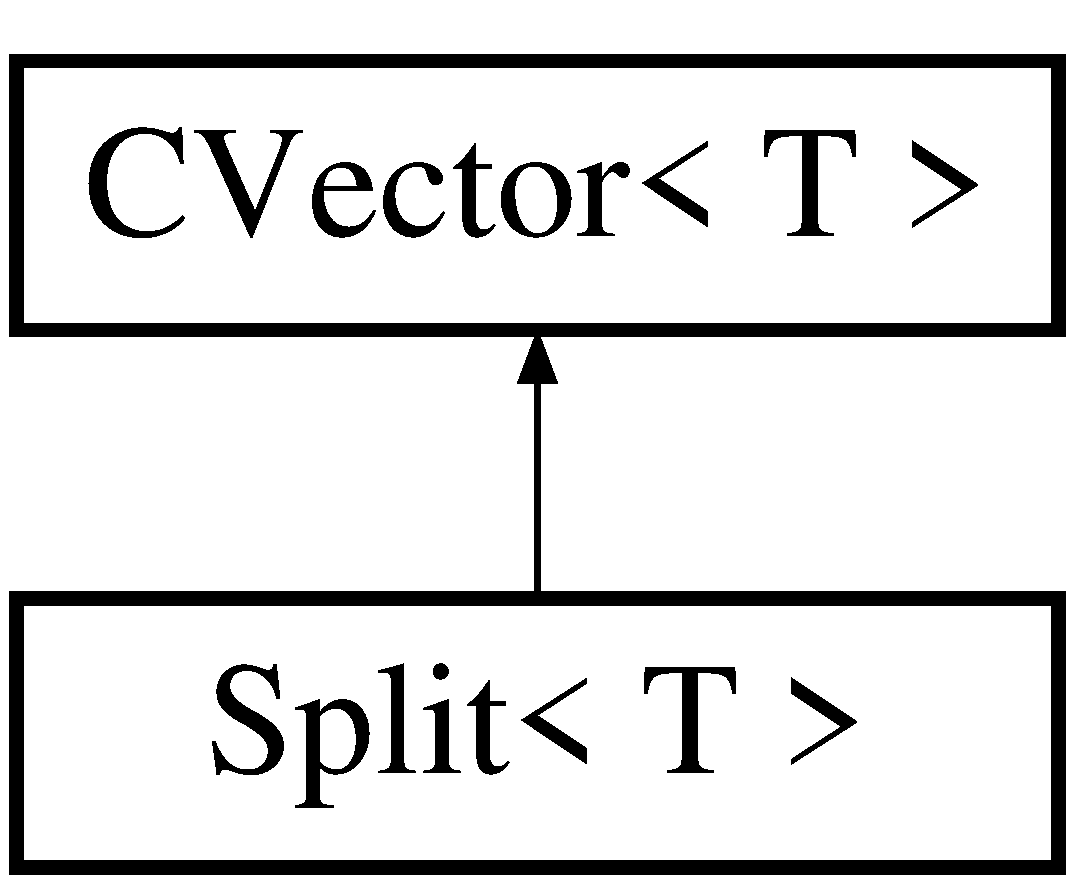
\includegraphics[height=2cm]{classCVector}
\end{center}
\end{figure}
\subsection*{Public Member Functions}
\begin{CompactItemize}
\item 
{\bf CVector} ()
\item 
{\bf CVector} (const {\bf CVector} \&)
\item 
{\bf CVector} (size\_\-t)
\item 
{\bf $\sim$CVector} ()
\item 
{\bf CVector} \& {\bf operator=} (const {\bf CVector} \&)
\item 
T \& {\bf operator[$\,$]} (size\_\-t)
\item 
T \& {\bf at} (size\_\-t)
\item 
const T \& {\bf operator[$\,$]} (size\_\-t) const 
\item 
const T \& {\bf at} (size\_\-t) const 
\item 
void {\bf push\_\-back} (const T \&)
\item 
void {\bf pop\_\-back} ()
\item 
void {\bf reserve} (size\_\-t)
\item 
void {\bf clear} ()
\item 
size\_\-t {\bf size} () const 
\item 
void {\bf set\-Size} (size\_\-t)
\item 
bool {\bf empty} () const 
\end{CompactItemize}
\subsection*{Static Public Attributes}
\begin{CompactItemize}
\item 
static double {\bf \_\-growth\-Factor} = 1.5
\begin{CompactList}\small\item\em Factor to use when resizing: \_\-size = \_\-growth\-Factor $\ast$ \_\-size. \item\end{CompactList}\end{CompactItemize}
\subsection*{Protected Member Functions}
\begin{CompactItemize}
\item 
void {\bf grow} ()
\end{CompactItemize}
\subsection*{Protected Attributes}
\begin{CompactItemize}
\item 
T $\ast$ {\bf \_\-array}
\item 
size\_\-t {\bf \_\-size}
\begin{CompactList}\small\item\em The actual memory block. \item\end{CompactList}\item 
size\_\-t {\bf \_\-cap}
\begin{CompactList}\small\item\em The number of elements. \item\end{CompactList}\end{CompactItemize}


\subsection{Detailed Description}
\subsubsection*{template$<$class T$>$ class CVector$<$ T $>$}

This is a c-style implementation of std::vector. 

It is designed for PODs (plain old datatypes) ie objects without constructors and uses realloc() to request new memory. The assumption is realloc() is potentially more efficient than new() as it can sometimes increase the reserved memory without having to copy the current contents. 



\subsection{Constructor \& Destructor Documentation}
\index{CVector@{CVector}!CVector@{CVector}}
\index{CVector@{CVector}!CVector@{CVector}}
\subsubsection{\setlength{\rightskip}{0pt plus 5cm}template$<$class T$>$ {\bf CVector}$<$ T $>$::{\bf CVector} ()\hspace{0.3cm}{\tt  [inline]}}\label{classCVector_a0}


\index{CVector@{CVector}!CVector@{CVector}}
\index{CVector@{CVector}!CVector@{CVector}}
\subsubsection{\setlength{\rightskip}{0pt plus 5cm}template$<$class T$>$ {\bf CVector}$<$ T $>$::{\bf CVector} (const {\bf CVector}$<$ T $>$ \&)\hspace{0.3cm}{\tt  [inline]}}\label{classCVector_a1}


\index{CVector@{CVector}!CVector@{CVector}}
\index{CVector@{CVector}!CVector@{CVector}}
\subsubsection{\setlength{\rightskip}{0pt plus 5cm}template$<$class T$>$ {\bf CVector}$<$ T $>$::{\bf CVector} (size\_\-t)\hspace{0.3cm}{\tt  [inline]}}\label{classCVector_a2}


\index{CVector@{CVector}!~CVector@{$\sim$CVector}}
\index{~CVector@{$\sim$CVector}!CVector@{CVector}}
\subsubsection{\setlength{\rightskip}{0pt plus 5cm}template$<$class T$>$ {\bf CVector}$<$ T $>$::$\sim${\bf CVector} ()\hspace{0.3cm}{\tt  [inline]}}\label{classCVector_a3}




\subsection{Member Function Documentation}
\index{CVector@{CVector}!at@{at}}
\index{at@{at}!CVector@{CVector}}
\subsubsection{\setlength{\rightskip}{0pt plus 5cm}template$<$class T$>$ const T \& {\bf CVector}$<$ T $>$::at (size\_\-t) const\hspace{0.3cm}{\tt  [inline]}}\label{classCVector_a8}


\index{CVector@{CVector}!at@{at}}
\index{at@{at}!CVector@{CVector}}
\subsubsection{\setlength{\rightskip}{0pt plus 5cm}template$<$class T$>$ T \& {\bf CVector}$<$ T $>$::at (size\_\-t)\hspace{0.3cm}{\tt  [inline]}}\label{classCVector_a6}


\index{CVector@{CVector}!clear@{clear}}
\index{clear@{clear}!CVector@{CVector}}
\subsubsection{\setlength{\rightskip}{0pt plus 5cm}template$<$class T$>$ void {\bf CVector}$<$ T $>$::clear ()\hspace{0.3cm}{\tt  [inline]}}\label{classCVector_a12}


\index{CVector@{CVector}!empty@{empty}}
\index{empty@{empty}!CVector@{CVector}}
\subsubsection{\setlength{\rightskip}{0pt plus 5cm}template$<$class T$>$ bool {\bf CVector}$<$ T $>$::empty () const\hspace{0.3cm}{\tt  [inline]}}\label{classCVector_a15}


\index{CVector@{CVector}!grow@{grow}}
\index{grow@{grow}!CVector@{CVector}}
\subsubsection{\setlength{\rightskip}{0pt plus 5cm}template$<$class T$>$ void {\bf CVector}$<$ T $>$::grow ()\hspace{0.3cm}{\tt  [protected]}}\label{classCVector_b0}


\index{CVector@{CVector}!operator=@{operator=}}
\index{operator=@{operator=}!CVector@{CVector}}
\subsubsection{\setlength{\rightskip}{0pt plus 5cm}template$<$class T$>$ {\bf CVector}$<$ T $>$ \& {\bf CVector}$<$ T $>$::operator= (const {\bf CVector}$<$ T $>$ \&)\hspace{0.3cm}{\tt  [inline]}}\label{classCVector_a4}


\index{CVector@{CVector}!operator[]@{operator[]}}
\index{operator[]@{operator[]}!CVector@{CVector}}
\subsubsection{\setlength{\rightskip}{0pt plus 5cm}template$<$class T$>$ const T \& {\bf CVector}$<$ T $>$::operator[$\,$] (size\_\-t) const\hspace{0.3cm}{\tt  [inline]}}\label{classCVector_a7}


\index{CVector@{CVector}!operator[]@{operator[]}}
\index{operator[]@{operator[]}!CVector@{CVector}}
\subsubsection{\setlength{\rightskip}{0pt plus 5cm}template$<$class T$>$ T \& {\bf CVector}$<$ T $>$::operator[$\,$] (size\_\-t)\hspace{0.3cm}{\tt  [inline]}}\label{classCVector_a5}


\index{CVector@{CVector}!pop_back@{pop\_\-back}}
\index{pop_back@{pop\_\-back}!CVector@{CVector}}
\subsubsection{\setlength{\rightskip}{0pt plus 5cm}template$<$class T$>$ void {\bf CVector}$<$ T $>$::pop\_\-back ()\hspace{0.3cm}{\tt  [inline]}}\label{classCVector_a10}


\index{CVector@{CVector}!push_back@{push\_\-back}}
\index{push_back@{push\_\-back}!CVector@{CVector}}
\subsubsection{\setlength{\rightskip}{0pt plus 5cm}template$<$class T$>$ void {\bf CVector}$<$ T $>$::push\_\-back (const T \&)\hspace{0.3cm}{\tt  [inline]}}\label{classCVector_a9}


\index{CVector@{CVector}!reserve@{reserve}}
\index{reserve@{reserve}!CVector@{CVector}}
\subsubsection{\setlength{\rightskip}{0pt plus 5cm}template$<$class T$>$ void {\bf CVector}$<$ T $>$::reserve (size\_\-t)\hspace{0.3cm}{\tt  [inline]}}\label{classCVector_a11}


\index{CVector@{CVector}!setSize@{setSize}}
\index{setSize@{setSize}!CVector@{CVector}}
\subsubsection{\setlength{\rightskip}{0pt plus 5cm}template$<$class T$>$ void {\bf CVector}$<$ T $>$::set\-Size (size\_\-t)\hspace{0.3cm}{\tt  [inline]}}\label{classCVector_a14}


\index{CVector@{CVector}!size@{size}}
\index{size@{size}!CVector@{CVector}}
\subsubsection{\setlength{\rightskip}{0pt plus 5cm}template$<$class T$>$ size\_\-t {\bf CVector}$<$ T $>$::size () const\hspace{0.3cm}{\tt  [inline]}}\label{classCVector_a13}




\subsection{Member Data Documentation}
\index{CVector@{CVector}!_array@{\_\-array}}
\index{_array@{\_\-array}!CVector@{CVector}}
\subsubsection{\setlength{\rightskip}{0pt plus 5cm}template$<$class T$>$ T$\ast$ {\bf CVector}$<$ T $>$::{\bf \_\-array}\hspace{0.3cm}{\tt  [protected]}}\label{classCVector_p0}


\index{CVector@{CVector}!_cap@{\_\-cap}}
\index{_cap@{\_\-cap}!CVector@{CVector}}
\subsubsection{\setlength{\rightskip}{0pt plus 5cm}template$<$class T$>$ size\_\-t {\bf CVector}$<$ T $>$::{\bf \_\-cap}\hspace{0.3cm}{\tt  [protected]}}\label{classCVector_p2}


The number of elements. 

\index{CVector@{CVector}!_growthFactor@{\_\-growthFactor}}
\index{_growthFactor@{\_\-growthFactor}!CVector@{CVector}}
\subsubsection{\setlength{\rightskip}{0pt plus 5cm}template$<$class T$>$ double {\bf CVector}$<$ T $>$::{\bf \_\-growth\-Factor} = 1.5\hspace{0.3cm}{\tt  [static]}}\label{classCVector_s0}


Factor to use when resizing: \_\-size = \_\-growth\-Factor $\ast$ \_\-size. 

\index{CVector@{CVector}!_size@{\_\-size}}
\index{_size@{\_\-size}!CVector@{CVector}}
\subsubsection{\setlength{\rightskip}{0pt plus 5cm}template$<$class T$>$ size\_\-t {\bf CVector}$<$ T $>$::{\bf \_\-size}\hspace{0.3cm}{\tt  [protected]}}\label{classCVector_p1}


The actual memory block. 



The documentation for this class was generated from the following files:\begin{CompactItemize}
\item 
{\bf cvector.h}\item 
{\bf cvector\_\-impl.h}\end{CompactItemize}

\section{Extract\-Splits\-Forest Class Reference}
\label{classExtractSplitsForest}\index{ExtractSplitsForest@{ExtractSplitsForest}}
{\tt \#include $<$extractsplitsforest.h$>$}

\subsection*{Public Member Functions}
\begin{CompactItemize}
\item 
{\bf Extract\-Splits\-Forest} ()
\item 
{\bf $\sim$Extract\-Splits\-Forest} ()
\item 
int {\bf extract} (const std::string \&, const std::string \&, std::vector$<$ std::string $>$ \&, std::vector$<$ std::string $>$ \&)
\begin{CompactList}\small\item\em Find the common splits forest for a pair of trees. \item\end{CompactList}\end{CompactItemize}
\subsection*{Protected Member Functions}
\begin{CompactItemize}
\item 
int {\bf get\-Splits} (const std::vector$<$ std::string $>$ \&, std::set$<$ {\bf Split} $\ast$, {\bf Split\-PLess} $>$ \&)
\begin{CompactList}\small\item\em Extract the splits from a tree. \item\end{CompactList}\item 
bool {\bf break\-LCS} (const std::vector$<$ std::string $>$ \&, const std::vector$<$ std::string $>$ \&tree2, std::vector$<$ std::string $>$ \&, std::vector$<$ std::string $>$ \&, std::vector$<$ std::string $>$ \&, std::vector$<$ std::string $>$ \&)
\item 
void {\bf split\-Tree} (const std::vector$<$ std::string $>$ \&, const {\bf Split} \&, std::vector$<$ std::string $>$ \&, std::vector$<$ std::string $>$ \&)
\end{CompactItemize}
\subsection*{Protected Attributes}
\begin{CompactItemize}
\item 
std::vector$<$ std::string $>$ {\bf \_\-temp}
\item 
int {\bf \_\-next\-Label}
\end{CompactItemize}


\subsection{Constructor \& Destructor Documentation}
\index{ExtractSplitsForest@{Extract\-Splits\-Forest}!ExtractSplitsForest@{ExtractSplitsForest}}
\index{ExtractSplitsForest@{ExtractSplitsForest}!ExtractSplitsForest@{Extract\-Splits\-Forest}}
\subsubsection{\setlength{\rightskip}{0pt plus 5cm}Extract\-Splits\-Forest::Extract\-Splits\-Forest ()}\label{classExtractSplitsForest_a0}


\index{ExtractSplitsForest@{Extract\-Splits\-Forest}!~ExtractSplitsForest@{$\sim$ExtractSplitsForest}}
\index{~ExtractSplitsForest@{$\sim$ExtractSplitsForest}!ExtractSplitsForest@{Extract\-Splits\-Forest}}
\subsubsection{\setlength{\rightskip}{0pt plus 5cm}Extract\-Splits\-Forest::$\sim${\bf Extract\-Splits\-Forest} ()}\label{classExtractSplitsForest_a1}




\subsection{Member Function Documentation}
\index{ExtractSplitsForest@{Extract\-Splits\-Forest}!breakLCS@{breakLCS}}
\index{breakLCS@{breakLCS}!ExtractSplitsForest@{Extract\-Splits\-Forest}}
\subsubsection{\setlength{\rightskip}{0pt plus 5cm}bool Extract\-Splits\-Forest::break\-LCS (const std::vector$<$ std::string $>$ \&, const std::vector$<$ std::string $>$ \& {\em tree2}, std::vector$<$ std::string $>$ \&, std::vector$<$ std::string $>$ \&, std::vector$<$ std::string $>$ \&, std::vector$<$ std::string $>$ \&)\hspace{0.3cm}{\tt  [protected]}}\label{classExtractSplitsForest_b1}


\index{ExtractSplitsForest@{Extract\-Splits\-Forest}!extract@{extract}}
\index{extract@{extract}!ExtractSplitsForest@{Extract\-Splits\-Forest}}
\subsubsection{\setlength{\rightskip}{0pt plus 5cm}int Extract\-Splits\-Forest::extract (const std::string \& {\em t1}, const std::string \& {\em t2}, std::vector$<$ std::string $>$ \& {\em f1}, std::vector$<$ std::string $>$ \& {\em f2})}\label{classExtractSplitsForest_a2}


Find the common splits forest for a pair of trees. 

\index{ExtractSplitsForest@{Extract\-Splits\-Forest}!getSplits@{getSplits}}
\index{getSplits@{getSplits}!ExtractSplitsForest@{Extract\-Splits\-Forest}}
\subsubsection{\setlength{\rightskip}{0pt plus 5cm}int Extract\-Splits\-Forest::get\-Splits (const std::vector$<$ std::string $>$ \& {\em tree}, std::set$<$ {\bf Split} $\ast$, {\bf Split\-PLess} $>$ \& {\em splitset})\hspace{0.3cm}{\tt  [protected]}}\label{classExtractSplitsForest_b0}


Extract the splits from a tree. 

There should be one for each INTERNAL edge wich is n-3 or something. \index{ExtractSplitsForest@{Extract\-Splits\-Forest}!splitTree@{splitTree}}
\index{splitTree@{splitTree}!ExtractSplitsForest@{Extract\-Splits\-Forest}}
\subsubsection{\setlength{\rightskip}{0pt plus 5cm}void Extract\-Splits\-Forest::split\-Tree (const std::vector$<$ std::string $>$ \&, const {\bf Split} \&, std::vector$<$ std::string $>$ \&, std::vector$<$ std::string $>$ \&)\hspace{0.3cm}{\tt  [protected]}}\label{classExtractSplitsForest_b2}




\subsection{Member Data Documentation}
\index{ExtractSplitsForest@{Extract\-Splits\-Forest}!_nextLabel@{\_\-nextLabel}}
\index{_nextLabel@{\_\-nextLabel}!ExtractSplitsForest@{Extract\-Splits\-Forest}}
\subsubsection{\setlength{\rightskip}{0pt plus 5cm}int {\bf Extract\-Splits\-Forest::\_\-next\-Label}\hspace{0.3cm}{\tt  [protected]}}\label{classExtractSplitsForest_p1}


\index{ExtractSplitsForest@{Extract\-Splits\-Forest}!_temp@{\_\-temp}}
\index{_temp@{\_\-temp}!ExtractSplitsForest@{Extract\-Splits\-Forest}}
\subsubsection{\setlength{\rightskip}{0pt plus 5cm}std::vector$<$std::string$>$ {\bf Extract\-Splits\-Forest::\_\-temp}\hspace{0.3cm}{\tt  [protected]}}\label{classExtractSplitsForest_p0}




The documentation for this class was generated from the following files:\begin{CompactItemize}
\item 
{\bf extractsplitsforest.h}\item 
{\bf extractsplitsforest.cpp}\item 
{\bf extractsplitsforest\_\-impl.h}\end{CompactItemize}

\section{Extract\-Subtree$<$ T, U $>$ Class Template Reference}
\label{classExtractSubtree}\index{ExtractSubtree@{ExtractSubtree}}
{\tt \#include $<$extractsubtree.h$>$}

\subsection*{Public Member Functions}
\begin{CompactItemize}
\item 
{\bf Extract\-Subtree} ()
\item 
{\bf $\sim$Extract\-Subtree} ()
\item 
bool {\bf extract} (const {\bf UPTree}$<$ U $>$ \&, const std::vector$<$ std::string $>$ \&, const {\bf UPTree}$<$ T $>$ \&, const std::vector$<$ std::string $>$ \&, std::string \&)
\begin{CompactList}\small\item\em Removes all leaves from supertree that are not present in reftree and copies the results into otree. \item\end{CompactList}\end{CompactItemize}
\subsection*{Protected Attributes}
\begin{CompactItemize}
\item 
{\bf Bracket\-Table}$<$ U $>$ {\bf \_\-btable}
\item 
{\bf Flag\-Table}$<$ U $>$ {\bf \_\-ftable}
\item 
std::set$<$ std::string $>$ {\bf \_\-set}
\end{CompactItemize}
\subsubsection*{template$<$class T, class U$>$ class Extract\-Subtree$<$ T, U $>$}



\subsection{Constructor \& Destructor Documentation}
\index{ExtractSubtree@{Extract\-Subtree}!ExtractSubtree@{ExtractSubtree}}
\index{ExtractSubtree@{ExtractSubtree}!ExtractSubtree@{Extract\-Subtree}}
\subsubsection{\setlength{\rightskip}{0pt plus 5cm}template$<$class T, class U$>$ {\bf Extract\-Subtree}$<$ T, U $>$::{\bf Extract\-Subtree} ()}\label{classExtractSubtree_a0}


\index{ExtractSubtree@{Extract\-Subtree}!~ExtractSubtree@{$\sim$ExtractSubtree}}
\index{~ExtractSubtree@{$\sim$ExtractSubtree}!ExtractSubtree@{Extract\-Subtree}}
\subsubsection{\setlength{\rightskip}{0pt plus 5cm}template$<$class T, class U$>$ {\bf Extract\-Subtree}$<$ T, U $>$::$\sim${\bf Extract\-Subtree} ()}\label{classExtractSubtree_a1}




\subsection{Member Function Documentation}
\index{ExtractSubtree@{Extract\-Subtree}!extract@{extract}}
\index{extract@{extract}!ExtractSubtree@{Extract\-Subtree}}
\subsubsection{\setlength{\rightskip}{0pt plus 5cm}template$<$class T, class U$>$ bool {\bf Extract\-Subtree}$<$ T, U $>$::extract (const {\bf UPTree}$<$ U $>$ \& {\em super\-Tree}, const std::vector$<$ std::string $>$ \& {\em super\-Lookup}, const {\bf UPTree}$<$ T $>$ \& {\em ref\-Tree}, const std::vector$<$ std::string $>$ \& {\em ref\-Lookup}, std::string \& {\em otree})}\label{classExtractSubtree_a2}


Removes all leaves from supertree that are not present in reftree and copies the results into otree. 

Note that each leaf removal is accompanied by the corresponding edge contraction. It assumed that input trees are numbered from 0 to numleaves-1. The lookup tables are used to access original values. \begin{Desc}
\item[Parameters:]
\begin{description}
\item[{\em super\-Tree}]The supertree to extract from \item[{\em super\-Lookup}]Name map for supertree \item[{\em ref\-Tree}]The tree whose leafset is to be extracted \item[{\em ref\-Lookup}]Name map for reference tree \item[{\em otree}]The output tree in string format \end{description}
\end{Desc}
\begin{Desc}
\item[Returns:]true if subtree of supertree with leaf set of reftree is successfully extracted. \end{Desc}


\subsection{Member Data Documentation}
\index{ExtractSubtree@{Extract\-Subtree}!_btable@{\_\-btable}}
\index{_btable@{\_\-btable}!ExtractSubtree@{Extract\-Subtree}}
\subsubsection{\setlength{\rightskip}{0pt plus 5cm}template$<$class T, class U$>$ {\bf Bracket\-Table}$<$U$>$ {\bf Extract\-Subtree}$<$ T, U $>$::{\bf \_\-btable}\hspace{0.3cm}{\tt  [protected]}}\label{classExtractSubtree_p0}


\index{ExtractSubtree@{Extract\-Subtree}!_ftable@{\_\-ftable}}
\index{_ftable@{\_\-ftable}!ExtractSubtree@{Extract\-Subtree}}
\subsubsection{\setlength{\rightskip}{0pt plus 5cm}template$<$class T, class U$>$ {\bf Flag\-Table}$<$U$>$ {\bf Extract\-Subtree}$<$ T, U $>$::{\bf \_\-ftable}\hspace{0.3cm}{\tt  [protected]}}\label{classExtractSubtree_p1}


\index{ExtractSubtree@{Extract\-Subtree}!_set@{\_\-set}}
\index{_set@{\_\-set}!ExtractSubtree@{Extract\-Subtree}}
\subsubsection{\setlength{\rightskip}{0pt plus 5cm}template$<$class T, class U$>$ std::set$<$std::string$>$ {\bf Extract\-Subtree}$<$ T, U $>$::{\bf \_\-set}\hspace{0.3cm}{\tt  [protected]}}\label{classExtractSubtree_p2}




The documentation for this class was generated from the following files:\begin{CompactItemize}
\item 
{\bf extractsubtree.h}\item 
{\bf extractsubtree\_\-impl.h}\end{CompactItemize}

\section{Flag\-Table$<$ T $>$ Class Template Reference}
\label{classFlagTable}\index{FlagTable@{FlagTable}}
This class keeps track of a boolean flag for each element of a tree string.  


{\tt \#include $<$flagtable.h$>$}

\subsection*{Public Member Functions}
\begin{CompactItemize}
\item 
{\bf Flag\-Table} ()
\item 
{\bf Flag\-Table} (int)
\item 
{\bf $\sim$Flag\-Table} ()
\item 
void {\bf resize} (int)
\begin{CompactList}\small\item\em Resize table if necessary. \item\end{CompactList}\item 
void {\bf set\-All} (bool, bool)
\begin{CompactList}\small\item\em Set all flags in the table. \item\end{CompactList}\item 
int {\bf load\-Tree} (const {\bf UPTree}$<$ T $>$ \&, const {\bf Bracket\-Table}$<$ T $>$ \&)
\begin{CompactList}\small\item\em Load a tree and compute the cherry position of all leaves. \item\end{CompactList}\item 
void {\bf copy} (const {\bf Flag\-Table}$<$ T $>$ \&, const int $\ast$)
\begin{CompactList}\small\item\em Copy the flags from a tree with a different topology. \item\end{CompactList}\item 
int {\bf left\-Pos} (int) const 
\item 
int {\bf right\-Pos} (int) const 
\item 
int {\bf cherry\-Pos} (int) const 
\begin{CompactList}\small\item\em Find the position of the cherry neighbour of the leaf at position pos in the tree, ignoring all flagged nodes. \item\end{CompactList}\item 
void {\bf flag\-Leaf} (int)
\begin{CompactList}\small\item\em {\bf Flag}{\rm (p.\,\pageref{structFlagTable_1_1Flag})} a leaf at position pos. \item\end{CompactList}\item 
void {\bf set\-Flag} (int, {\bf Flag})
\begin{CompactList}\small\item\em Assign flag value val to position pos. \item\end{CompactList}\item 
void {\bf set\-Frozen} (int, bool)
\begin{CompactList}\small\item\em Mark flag at pos as frozen. \item\end{CompactList}\item 
void {\bf set\-Del} (int, bool)
\begin{CompactList}\small\item\em Mark flag at pos for deletion. \item\end{CompactList}\item 
bool {\bf is\-Frozen} (int) const 
\item 
bool {\bf is\-Del} (int) const 
\item 
{\bf Flag} {\bf flag} (int) const 
\item 
{\bf Flag} {\bf operator[$\,$]} (int) const 
\item 
void {\bf nest\-Pos} (int, int[2]) const 
\item 
void {\bf set\-Rule\-State} (unsigned char)
\item 
void {\bf update\-Rekern} ()
\item 
int {\bf get\-Right\-Pos} (int)
\begin{CompactList}\small\item\em Finds the right nested subtree of a subtree, making sure to ignore flagged elements. \item\end{CompactList}\end{CompactItemize}
\subsection*{Protected Member Functions}
\begin{CompactItemize}
\item 
void {\bf flag\-Update\-Neighbours} (int)
\begin{CompactList}\small\item\em Set the flag to freeze \& delete at a position and update its neighbours' neighbours to skip it. \item\end{CompactList}\end{CompactItemize}
\subsection*{Protected Attributes}
\begin{CompactItemize}
\item 
int {\bf \_\-size}
\item 
{\bf Neighbours} $\ast$ {\bf \_\-neis}
\begin{CompactList}\small\item\em Size of the table. \item\end{CompactList}\item 
{\bf Flag} $\ast$ {\bf \_\-flags}
\begin{CompactList}\small\item\em Table of left and right neighbour positions. \item\end{CompactList}\item 
const {\bf UPTree}$<$ T $>$ $\ast$ {\bf \_\-tree}
\begin{CompactList}\small\item\em Table of flags. \item\end{CompactList}\item 
const {\bf Bracket\-Table}$<$ T $>$ $\ast$ {\bf \_\-btable}
\begin{CompactList}\small\item\em Corresponding tree. \item\end{CompactList}\item 
int {\bf \_\-tri\-Pos} [3]
\begin{CompactList}\small\item\em Brackettable of \_\-tree. \item\end{CompactList}\item 
unsigned char {\bf \_\-rule\-State}
\begin{CompactList}\small\item\em Position of trifurcation subtrees in FLAGGED tree. \item\end{CompactList}\end{CompactItemize}
\subsection*{Friends}
\begin{CompactItemize}
\item 
std::ostream \& {\bf operator} (std::ostream \&, const {\bf Flag\-Table}$<$ T $>$ \&)
\end{CompactItemize}
\subsection*{Classes}
\begin{CompactItemize}
\item 
struct {\bf Flag}
\begin{CompactList}\small\item\em {\bf Flag}{\rm (p.\,\pageref{structFlagTable_1_1Flag})} can specify if a given node is marked as frozen and/or marked for deletion. \item\end{CompactList}\item 
struct {\bf Neighbours}
\begin{CompactList}\small\item\em Offset the next unflagged neighbour to the left and right of a position. \item\end{CompactList}\end{CompactItemize}


\subsection{Detailed Description}
\subsubsection*{template$<$class T$>$ class Flag\-Table$<$ T $>$}

This class keeps track of a boolean flag for each element of a tree string. 

Tt also allows immediate access to the next unflagged neighbour in the string (on the left or right) side. Note that flagging a leaf also flags a corresponding bracket pair. This table is used in conjunction with the cherry table to perform Rule 1 in linear time. 



\subsection{Constructor \& Destructor Documentation}
\index{FlagTable@{Flag\-Table}!FlagTable@{FlagTable}}
\index{FlagTable@{FlagTable}!FlagTable@{Flag\-Table}}
\subsubsection{\setlength{\rightskip}{0pt plus 5cm}template$<$class T$>$ {\bf Flag\-Table}$<$ T $>$::{\bf Flag\-Table} ()}\label{classFlagTable_a0}


\index{FlagTable@{Flag\-Table}!FlagTable@{FlagTable}}
\index{FlagTable@{FlagTable}!FlagTable@{Flag\-Table}}
\subsubsection{\setlength{\rightskip}{0pt plus 5cm}template$<$class T$>$ {\bf Flag\-Table}$<$ T $>$::{\bf Flag\-Table} (int {\em size})}\label{classFlagTable_a1}


\begin{Desc}
\item[Parameters:]
\begin{description}
\item[{\em size}]Size of table to create. \end{description}
\end{Desc}
\index{FlagTable@{Flag\-Table}!~FlagTable@{$\sim$FlagTable}}
\index{~FlagTable@{$\sim$FlagTable}!FlagTable@{Flag\-Table}}
\subsubsection{\setlength{\rightskip}{0pt plus 5cm}template$<$class T$>$ {\bf Flag\-Table}$<$ T $>$::$\sim${\bf Flag\-Table} ()}\label{classFlagTable_a2}




\subsection{Member Function Documentation}
\index{FlagTable@{Flag\-Table}!cherryPos@{cherryPos}}
\index{cherryPos@{cherryPos}!FlagTable@{Flag\-Table}}
\subsubsection{\setlength{\rightskip}{0pt plus 5cm}template$<$class T$>$ int {\bf Flag\-Table}$<$ T $>$::cherry\-Pos (int {\em pos}) const}\label{classFlagTable_a9}


Find the position of the cherry neighbour of the leaf at position pos in the tree, ignoring all flagged nodes. 

\begin{Desc}
\item[Returns:]Position of cherry neighbour of -1 if it does not exist. \end{Desc}
\index{FlagTable@{Flag\-Table}!copy@{copy}}
\index{copy@{copy}!FlagTable@{Flag\-Table}}
\subsubsection{\setlength{\rightskip}{0pt plus 5cm}template$<$class T$>$ void {\bf Flag\-Table}$<$ T $>$::copy (const {\bf Flag\-Table}$<$ T $>$ \& {\em ftable}, const int $\ast$ {\em lookup})}\label{classFlagTable_a6}


Copy the flags from a tree with a different topology. 

This is acccomplisehd by reflagging each leaf that was flagged for deletion along with its brackets. Frozen leaves are kept frozen without touching brackets. {\bf update\-Rekern()}{\rm (p.\,\pageref{classFlagTable_a20})} may have to be called again. \index{FlagTable@{Flag\-Table}!flag@{flag}}
\index{flag@{flag}!FlagTable@{Flag\-Table}}
\subsubsection{\setlength{\rightskip}{0pt plus 5cm}template$<$class T$>$ {\bf Flag\-Table}$<$ T $>$::{\bf Flag} {\bf Flag\-Table}$<$ T $>$::flag (int {\em pos}) const\hspace{0.3cm}{\tt  [inline]}}\label{classFlagTable_a16}


\begin{Desc}
\item[Returns:]Boolean flag value at position pos. \end{Desc}
\index{FlagTable@{Flag\-Table}!flagLeaf@{flagLeaf}}
\index{flagLeaf@{flagLeaf}!FlagTable@{Flag\-Table}}
\subsubsection{\setlength{\rightskip}{0pt plus 5cm}template$<$class T$>$ void {\bf Flag\-Table}$<$ T $>$::flag\-Leaf (int {\em pos})}\label{classFlagTable_a10}


{\bf Flag}{\rm (p.\,\pageref{structFlagTable_1_1Flag})} a leaf at position pos. 

The structure is then updated to reflect a tree from which this leaf has been deleted. This means that an edge (pair of brackets) is also flagged and all left/right neighbours are updated to skip the flagged nodes. Finally, the start positions of the trifurcation subtrees are updated. Positions are flagged as both freeze and delete. Fine-tuning is done manually using the set methods. \index{FlagTable@{Flag\-Table}!flagUpdateNeighbours@{flagUpdateNeighbours}}
\index{flagUpdateNeighbours@{flagUpdateNeighbours}!FlagTable@{Flag\-Table}}
\subsubsection{\setlength{\rightskip}{0pt plus 5cm}template$<$class T$>$ void {\bf Flag\-Table}$<$ T $>$::flag\-Update\-Neighbours (int {\em pos})\hspace{0.3cm}{\tt  [protected]}}\label{classFlagTable_b0}


Set the flag to freeze \& delete at a position and update its neighbours' neighbours to skip it. 

\index{FlagTable@{Flag\-Table}!getRightPos@{getRightPos}}
\index{getRightPos@{getRightPos}!FlagTable@{Flag\-Table}}
\subsubsection{\setlength{\rightskip}{0pt plus 5cm}template$<$class T$>$ int {\bf Flag\-Table}$<$ T $>$::get\-Right\-Pos (int {\em pos})}\label{classFlagTable_a21}


Finds the right nested subtree of a subtree, making sure to ignore flagged elements. 

\begin{Desc}
\item[Parameters:]
\begin{description}
\item[{\em pos}]Position of the leftbracket of the subtree \end{description}
\end{Desc}
\begin{Desc}
\item[Returns:]position of the right subtree of the input subtree \end{Desc}
\index{FlagTable@{Flag\-Table}!isDel@{isDel}}
\index{isDel@{isDel}!FlagTable@{Flag\-Table}}
\subsubsection{\setlength{\rightskip}{0pt plus 5cm}template$<$class T$>$ bool {\bf Flag\-Table}$<$ T $>$::is\-Del (int {\em pos}) const\hspace{0.3cm}{\tt  [inline]}}\label{classFlagTable_a15}


\begin{Desc}
\item[Returns:]true if position pos is marked for deletion \end{Desc}
\index{FlagTable@{Flag\-Table}!isFrozen@{isFrozen}}
\index{isFrozen@{isFrozen}!FlagTable@{Flag\-Table}}
\subsubsection{\setlength{\rightskip}{0pt plus 5cm}template$<$class T$>$ bool {\bf Flag\-Table}$<$ T $>$::is\-Frozen (int {\em pos}) const\hspace{0.3cm}{\tt  [inline]}}\label{classFlagTable_a14}


\begin{Desc}
\item[Returns:]true if position pos is marked as frozen \end{Desc}
\index{FlagTable@{Flag\-Table}!leftPos@{leftPos}}
\index{leftPos@{leftPos}!FlagTable@{Flag\-Table}}
\subsubsection{\setlength{\rightskip}{0pt plus 5cm}template$<$class T$>$ int {\bf Flag\-Table}$<$ T $>$::left\-Pos (int {\em pos}) const\hspace{0.3cm}{\tt  [inline]}}\label{classFlagTable_a7}


\begin{Desc}
\item[Returns:]Position of next unflagged neighbour to the left of pos. \end{Desc}
\index{FlagTable@{Flag\-Table}!loadTree@{loadTree}}
\index{loadTree@{loadTree}!FlagTable@{Flag\-Table}}
\subsubsection{\setlength{\rightskip}{0pt plus 5cm}template$<$class T$>$ int {\bf Flag\-Table}$<$ T $>$::load\-Tree (const {\bf UPTree}$<$ T $>$ \& {\em tree}, const {\bf Bracket\-Table}$<$ T $>$ \& {\em btable})}\label{classFlagTable_a5}


Load a tree and compute the cherry position of all leaves. 

Tree to load  Brackettable corresponding to tree. \index{FlagTable@{Flag\-Table}!nestPos@{nestPos}}
\index{nestPos@{nestPos}!FlagTable@{Flag\-Table}}
\subsubsection{\setlength{\rightskip}{0pt plus 5cm}template$<$class T$>$ void {\bf Flag\-Table}$<$ T $>$::nest\-Pos (int {\em pos}, int {\em nest}[2]) const}\label{classFlagTable_a18}


\index{FlagTable@{Flag\-Table}!operator[]@{operator[]}}
\index{operator[]@{operator[]}!FlagTable@{Flag\-Table}}
\subsubsection{\setlength{\rightskip}{0pt plus 5cm}template$<$class T$>$ {\bf Flag\-Table}$<$ T $>$::{\bf Flag} {\bf Flag\-Table}$<$ T $>$::operator[$\,$] (int {\em pos}) const\hspace{0.3cm}{\tt  [inline]}}\label{classFlagTable_a17}


\begin{Desc}
\item[Returns:]Boolean flag value at position pos. \end{Desc}
\index{FlagTable@{Flag\-Table}!resize@{resize}}
\index{resize@{resize}!FlagTable@{Flag\-Table}}
\subsubsection{\setlength{\rightskip}{0pt plus 5cm}template$<$class T$>$ void {\bf Flag\-Table}$<$ T $>$::resize (int {\em size})}\label{classFlagTable_a3}


Resize table if necessary. 

\index{FlagTable@{Flag\-Table}!rightPos@{rightPos}}
\index{rightPos@{rightPos}!FlagTable@{Flag\-Table}}
\subsubsection{\setlength{\rightskip}{0pt plus 5cm}template$<$class T$>$ int {\bf Flag\-Table}$<$ T $>$::right\-Pos (int {\em pos}) const\hspace{0.3cm}{\tt  [inline]}}\label{classFlagTable_a8}


\begin{Desc}
\item[Returns:]Position of next unflagged neighbour to the right of pos. \end{Desc}
\index{FlagTable@{Flag\-Table}!setAll@{setAll}}
\index{setAll@{setAll}!FlagTable@{Flag\-Table}}
\subsubsection{\setlength{\rightskip}{0pt plus 5cm}template$<$class T$>$ void {\bf Flag\-Table}$<$ T $>$::set\-All (bool {\em del}, bool {\em freeze})\hspace{0.3cm}{\tt  [inline]}}\label{classFlagTable_a4}


Set all flags in the table. 

\begin{Desc}
\item[Parameters:]
\begin{description}
\item[{\em val}]Value to assign to all flags. \end{description}
\end{Desc}
\index{FlagTable@{Flag\-Table}!setDel@{setDel}}
\index{setDel@{setDel}!FlagTable@{Flag\-Table}}
\subsubsection{\setlength{\rightskip}{0pt plus 5cm}template$<$class T$>$ void {\bf Flag\-Table}$<$ T $>$::set\-Del (int {\em pos}, bool {\em val})\hspace{0.3cm}{\tt  [inline]}}\label{classFlagTable_a13}


Mark flag at pos for deletion. 

\index{FlagTable@{Flag\-Table}!setFlag@{setFlag}}
\index{setFlag@{setFlag}!FlagTable@{Flag\-Table}}
\subsubsection{\setlength{\rightskip}{0pt plus 5cm}template$<$class T$>$ void {\bf Flag\-Table}$<$ T $>$::set\-Flag (int {\em pos}, {\bf Flag} {\em val})\hspace{0.3cm}{\tt  [inline]}}\label{classFlagTable_a11}


Assign flag value val to position pos. 

\index{FlagTable@{Flag\-Table}!setFrozen@{setFrozen}}
\index{setFrozen@{setFrozen}!FlagTable@{Flag\-Table}}
\subsubsection{\setlength{\rightskip}{0pt plus 5cm}template$<$class T$>$ void {\bf Flag\-Table}$<$ T $>$::set\-Frozen (int {\em pos}, bool {\em val})\hspace{0.3cm}{\tt  [inline]}}\label{classFlagTable_a12}


Mark flag at pos as frozen. 

\index{FlagTable@{Flag\-Table}!setRuleState@{setRuleState}}
\index{setRuleState@{setRuleState}!FlagTable@{Flag\-Table}}
\subsubsection{\setlength{\rightskip}{0pt plus 5cm}template$<$class T$>$ void {\bf Flag\-Table}$<$ T $>$::set\-Rule\-State (unsigned {\em char})}\label{classFlagTable_a19}


\index{FlagTable@{Flag\-Table}!updateRekern@{updateRekern}}
\index{updateRekern@{updateRekern}!FlagTable@{Flag\-Table}}
\subsubsection{\setlength{\rightskip}{0pt plus 5cm}template$<$class T$>$ void {\bf Flag\-Table}$<$ T $>$::update\-Rekern ()}\label{classFlagTable_a20}




\subsection{Friends And Related Function Documentation}
\index{FlagTable@{Flag\-Table}!operator@{operator}}
\index{operator@{operator}!FlagTable@{Flag\-Table}}
\subsubsection{\setlength{\rightskip}{0pt plus 5cm}template$<$class T$>$ std::ostream\& operator (std::ostream \&, const {\bf Flag\-Table}$<$ T $>$ \&)\hspace{0.3cm}{\tt  [friend]}}\label{classFlagTable_n0}




\subsection{Member Data Documentation}
\index{FlagTable@{Flag\-Table}!_btable@{\_\-btable}}
\index{_btable@{\_\-btable}!FlagTable@{Flag\-Table}}
\subsubsection{\setlength{\rightskip}{0pt plus 5cm}template$<$class T$>$ const {\bf Bracket\-Table}$<$T$>$$\ast$ {\bf Flag\-Table}$<$ T $>$::{\bf \_\-btable}\hspace{0.3cm}{\tt  [protected]}}\label{classFlagTable_p4}


Corresponding tree. 

\index{FlagTable@{Flag\-Table}!_flags@{\_\-flags}}
\index{_flags@{\_\-flags}!FlagTable@{Flag\-Table}}
\subsubsection{\setlength{\rightskip}{0pt plus 5cm}template$<$class T$>$ {\bf Flag}$\ast$ {\bf Flag\-Table}$<$ T $>$::{\bf \_\-flags}\hspace{0.3cm}{\tt  [protected]}}\label{classFlagTable_p2}


Table of left and right neighbour positions. 

\index{FlagTable@{Flag\-Table}!_neis@{\_\-neis}}
\index{_neis@{\_\-neis}!FlagTable@{Flag\-Table}}
\subsubsection{\setlength{\rightskip}{0pt plus 5cm}template$<$class T$>$ {\bf Neighbours}$\ast$ {\bf Flag\-Table}$<$ T $>$::{\bf \_\-neis}\hspace{0.3cm}{\tt  [protected]}}\label{classFlagTable_p1}


Size of the table. 

\index{FlagTable@{Flag\-Table}!_ruleState@{\_\-ruleState}}
\index{_ruleState@{\_\-ruleState}!FlagTable@{Flag\-Table}}
\subsubsection{\setlength{\rightskip}{0pt plus 5cm}template$<$class T$>$ unsigned char {\bf Flag\-Table}$<$ T $>$::{\bf \_\-rule\-State}\hspace{0.3cm}{\tt  [protected]}}\label{classFlagTable_p6}


Position of trifurcation subtrees in FLAGGED tree. 

\index{FlagTable@{Flag\-Table}!_size@{\_\-size}}
\index{_size@{\_\-size}!FlagTable@{Flag\-Table}}
\subsubsection{\setlength{\rightskip}{0pt plus 5cm}template$<$class T$>$ int {\bf Flag\-Table}$<$ T $>$::{\bf \_\-size}\hspace{0.3cm}{\tt  [protected]}}\label{classFlagTable_p0}


\index{FlagTable@{Flag\-Table}!_tree@{\_\-tree}}
\index{_tree@{\_\-tree}!FlagTable@{Flag\-Table}}
\subsubsection{\setlength{\rightskip}{0pt plus 5cm}template$<$class T$>$ const {\bf UPTree}$<$T$>$$\ast$ {\bf Flag\-Table}$<$ T $>$::{\bf \_\-tree}\hspace{0.3cm}{\tt  [protected]}}\label{classFlagTable_p3}


Table of flags. 

\index{FlagTable@{Flag\-Table}!_triPos@{\_\-triPos}}
\index{_triPos@{\_\-triPos}!FlagTable@{Flag\-Table}}
\subsubsection{\setlength{\rightskip}{0pt plus 5cm}template$<$class T$>$ int {\bf Flag\-Table}$<$ T $>$::{\bf \_\-tri\-Pos}[3]\hspace{0.3cm}{\tt  [protected]}}\label{classFlagTable_p5}


Brackettable of \_\-tree. 



The documentation for this class was generated from the following files:\begin{CompactItemize}
\item 
{\bf flagtable.h}\item 
{\bf flagtable\_\-impl.h}\end{CompactItemize}

\section{Flag\-Table$<$ T $>$::Flag$<$ T $>$ Struct Template Reference}
\label{structFlagTable_1_1Flag}\index{FlagTable::Flag@{FlagTable::Flag}}
{\bf Flag}{\rm (p.\,\pageref{structFlagTable_1_1Flag})} can specify if a given node is marked as frozen and/or marked for deletion.  


{\tt \#include $<$flagtable.h$>$}

\subsection*{Public Attributes}
\begin{CompactItemize}
\item 
unsigned char {\bf \_\-del}: 1
\item 
unsigned char {\bf \_\-freeze}: 1
\begin{CompactList}\small\item\em Marked for deletion (1: marked, 0: not). \item\end{CompactList}\item 
unsigned char {\bf \_\-rule}: 1
\begin{CompactList}\small\item\em Marked as frozen (1: marked, 0: not). \item\end{CompactList}\end{CompactItemize}


\subsection{Detailed Description}
\subsubsection*{template$<$class T$>$template$<$class T$>$ struct Flag\-Table$<$ T $>$::Flag$<$ T $>$}

{\bf Flag}{\rm (p.\,\pageref{structFlagTable_1_1Flag})} can specify if a given node is marked as frozen and/or marked for deletion. 

The two flags are required as there are some small differences between kernelization and rekernelization Most nodes will be flagged as both except: 1) An extra Freeze flag is applied to the beginning of common chains flagged by rule 2. So if c\_\-3, c\_\-4, ..., c\_\-x are flagged for deletion then c\_\-2 will also be flagged as freeze-only 2) All elements, including surrounding brackets, of common subtrees are flagged for deleltion by rule 1 except for the leaf with the lowest lable. For purposes of rekernelization, this leaf is also flagged as frozen but the surrounding brackets are unflagged. 



\subsection{Member Data Documentation}
\index{FlagTable::Flag@{Flag\-Table::Flag}!_del@{\_\-del}}
\index{_del@{\_\-del}!FlagTable::Flag@{Flag\-Table::Flag}}
\subsubsection{\setlength{\rightskip}{0pt plus 5cm}template$<$class T$>$ template$<$class T$>$ unsigned char {\bf Flag\-Table}$<$ T $>$::{\bf Flag}$<$ T $>$::{\bf \_\-del}}\label{structFlagTable_1_1Flag_o0}


\index{FlagTable::Flag@{Flag\-Table::Flag}!_freeze@{\_\-freeze}}
\index{_freeze@{\_\-freeze}!FlagTable::Flag@{Flag\-Table::Flag}}
\subsubsection{\setlength{\rightskip}{0pt plus 5cm}template$<$class T$>$ template$<$class T$>$ unsigned char {\bf Flag\-Table}$<$ T $>$::{\bf Flag}$<$ T $>$::{\bf \_\-freeze}}\label{structFlagTable_1_1Flag_o1}


Marked for deletion (1: marked, 0: not). 

\index{FlagTable::Flag@{Flag\-Table::Flag}!_rule@{\_\-rule}}
\index{_rule@{\_\-rule}!FlagTable::Flag@{Flag\-Table::Flag}}
\subsubsection{\setlength{\rightskip}{0pt plus 5cm}template$<$class T$>$ template$<$class T$>$ unsigned char {\bf Flag\-Table}$<$ T $>$::{\bf Flag}$<$ T $>$::{\bf \_\-rule}}\label{structFlagTable_1_1Flag_o2}


Marked as frozen (1: marked, 0: not). 



The documentation for this struct was generated from the following file:\begin{CompactItemize}
\item 
{\bf flagtable.h}\end{CompactItemize}

\section{Flag\-Table$<$ T $>$::Neighbours$<$ T $>$ Struct Template Reference}
\label{structFlagTable_1_1Neighbours}\index{FlagTable::Neighbours@{FlagTable::Neighbours}}
Offset the next unflagged neighbour to the left and right of a position.  


{\tt \#include $<$flagtable.h$>$}

\subsection*{Public Attributes}
\begin{CompactItemize}
\item 
int {\bf \_\-left}
\item 
int {\bf \_\-right}
\end{CompactItemize}


\subsection{Detailed Description}
\subsubsection*{template$<$class T$>$template$<$class T$>$ struct Flag\-Table$<$ T $>$::Neighbours$<$ T $>$}

Offset the next unflagged neighbour to the left and right of a position. 

This keeps cherry lookups in the flagged tree O(1). 



\subsection{Member Data Documentation}
\index{FlagTable::Neighbours@{Flag\-Table::Neighbours}!_left@{\_\-left}}
\index{_left@{\_\-left}!FlagTable::Neighbours@{Flag\-Table::Neighbours}}
\subsubsection{\setlength{\rightskip}{0pt plus 5cm}template$<$class T$>$ template$<$class T$>$ int {\bf Flag\-Table}$<$ T $>$::{\bf Neighbours}$<$ T $>$::{\bf \_\-left}}\label{structFlagTable_1_1Neighbours_o0}


\index{FlagTable::Neighbours@{Flag\-Table::Neighbours}!_right@{\_\-right}}
\index{_right@{\_\-right}!FlagTable::Neighbours@{Flag\-Table::Neighbours}}
\subsubsection{\setlength{\rightskip}{0pt plus 5cm}template$<$class T$>$ template$<$class T$>$ int {\bf Flag\-Table}$<$ T $>$::{\bf Neighbours}$<$ T $>$::{\bf \_\-right}}\label{structFlagTable_1_1Neighbours_o1}




The documentation for this struct was generated from the following file:\begin{CompactItemize}
\item 
{\bf flagtable.h}\end{CompactItemize}

\section{Kernelizor$<$ T $>$ Class Template Reference}
\label{classKernelizor}\index{Kernelizor@{Kernelizor}}
Kernelizes pairs of trees by flagging common subtrees and chains in accordance with Rule 1 and Rule 2.  


{\tt \#include $<$kernelizor.h$>$}

\subsection*{Public Member Functions}
\begin{CompactItemize}
\item 
{\bf Kernelizor} ({\bf Tree\-Manager}$<$ T $>$ \&)
\begin{CompactList}\small\item\em Construct the kernelizor. \item\end{CompactList}\item 
{\bf $\sim$Kernelizor} ()
\item 
void {\bf set\-T1} ({\bf UPTree}$<$ T $>$ \&)
\begin{CompactList}\small\item\em Set first tree of kernelization. \item\end{CompactList}\item 
void {\bf set\-T2} ({\bf UPTree}$<$ T $>$ \&)
\begin{CompactList}\small\item\em Set second tree of kernelization. \item\end{CompactList}\item 
int {\bf kernelize} ()
\begin{CompactList}\small\item\em Kernelize and return number of flagged leaves. \item\end{CompactList}\item 
size\_\-t {\bf num\-Leaves} () const 
\item 
const {\bf Bracket\-Table}$<$ T $>$ \& {\bf get\-BTable} (int) const 
\item 
const {\bf Flag\-Table}$<$ T $>$ \& {\bf get\-FTable} (int) const 
\item 
const int $\ast$ {\bf get\-Lookup} (int) const 
\end{CompactItemize}
\subsection*{Protected Member Functions}
\begin{CompactItemize}
\item 
void {\bf load\-Tree} ({\bf UPTree}$<$ T $>$ \&, int)
\begin{CompactList}\small\item\em Copy a reference of the tree into the slot corresponding to num and load all the relevant tables. \item\end{CompactList}\item 
int {\bf rule1} ()
\begin{CompactList}\small\item\em Flag all leaves but one in subtrees common to T1 and T2. \item\end{CompactList}\item 
int {\bf rule2} ()
\begin{CompactList}\small\item\em For each common chain c1,c2,c3...,ck in the (intermediate) trees, flag leaves c3,...,ck-1. \item\end{CompactList}\item 
int {\bf chain\-Links} (T, T[2])
\begin{CompactList}\small\item\em Use the chain tables to identify common chain neighbours of a leaf. \item\end{CompactList}\item 
int {\bf flag\-Chain} (T, T)
\begin{CompactList}\small\item\em Flag a common subchain in both trees. \item\end{CompactList}\item 
void {\bf copy\-To\-Temp} ()
\begin{CompactList}\small\item\em Copy the input trees (\_\-t[0] and \_\-t[1]) into the intermediate trees (\_\-t[2] and \_\-t[3]), ignoring flagged tokens. \item\end{CompactList}\item 
void {\bf copy\-From\-Temp} ()
\begin{CompactList}\small\item\em For every leaf flagged in the intermediate trees in Rule 2 but not flagged by Rule 1, flag in the original trees. \item\end{CompactList}\end{CompactItemize}
\subsection*{Protected Attributes}
\begin{CompactItemize}
\item 
{\bf UPTree}$<$ T $>$ {\bf \_\-t} [4]
\item 
{\bf Tree\-Manager}$<$ T $>$ $\ast$ {\bf \_\-man}
\begin{CompactList}\small\item\em \_\-t[0] \& \_\-t[1] are the input trees \_\-t[2] \& \_\-t[3] are the above after Rule1 \item\end{CompactList}\item 
size\_\-t {\bf \_\-num\-Leaves}
\begin{CompactList}\small\item\em tree manager to create \_\-t[2] and \_\-t[3] \item\end{CompactList}\item 
int {\bf \_\-temp\-Size}
\begin{CompactList}\small\item\em number of leaves in input trees \item\end{CompactList}\item 
int $\ast$ {\bf \_\-lookup} [4]
\begin{CompactList}\small\item\em number of leaves after Rule1 \item\end{CompactList}\item 
{\bf Bracket\-Table}$<$ T $>$ {\bf \_\-btable} [4]
\begin{CompactList}\small\item\em map label to position in all 4 trees \item\end{CompactList}\item 
{\bf Flag\-Table}$<$ T $>$ {\bf \_\-ftable} [4]
\begin{CompactList}\small\item\em bracket information tables \item\end{CompactList}\item 
{\bf Cherry\-Table}$<$ T $>$ {\bf \_\-cherry\-Table} [4]
\begin{CompactList}\small\item\em flag tables \item\end{CompactList}\item 
{\bf Chain\-Table}$<$ T $>$ {\bf \_\-chain\-Table} [4]
\begin{CompactList}\small\item\em cherry tables for Rule 1 \item\end{CompactList}\item 
std::queue$<$ int $>$ {\bf \_\-queue}
\begin{CompactList}\small\item\em chain tables for Rule 2 \item\end{CompactList}\end{CompactItemize}
\subsection*{Private Member Functions}
\begin{CompactItemize}
\item 
{\bf Kernelizor} ()
\begin{CompactList}\small\item\em queue used in rule 1 \item\end{CompactList}\end{CompactItemize}
\subsection*{Friends}
\begin{CompactItemize}
\item 
std::ostream \& {\bf operator} (std::ostream \&, {\bf Kernelizor}$<$ T $>$ \&)
\end{CompactItemize}


\subsection{Detailed Description}
\subsubsection*{template$<$class T$>$ class Kernelizor$<$ T $>$}

Kernelizes pairs of trees by flagging common subtrees and chains in accordance with Rule 1 and Rule 2. 

The time complexity is linear. 



\subsection{Constructor \& Destructor Documentation}
\index{Kernelizor@{Kernelizor}!Kernelizor@{Kernelizor}}
\index{Kernelizor@{Kernelizor}!Kernelizor@{Kernelizor}}
\subsubsection{\setlength{\rightskip}{0pt plus 5cm}template$<$class T$>$ {\bf Kernelizor}$<$ T $>$::{\bf Kernelizor} ({\bf Tree\-Manager}$<$ T $>$ \& {\em man})}\label{classKernelizor_a0}


Construct the kernelizor. 

Note the default constructor is disabled. \begin{Desc}
\item[Parameters:]
\begin{description}
\item[{\em man}]Tree manager. Must correspond to manager of input trees. \end{description}
\end{Desc}
\index{Kernelizor@{Kernelizor}!~Kernelizor@{$\sim$Kernelizor}}
\index{~Kernelizor@{$\sim$Kernelizor}!Kernelizor@{Kernelizor}}
\subsubsection{\setlength{\rightskip}{0pt plus 5cm}template$<$class T$>$ {\bf Kernelizor}$<$ T $>$::$\sim${\bf Kernelizor} ()}\label{classKernelizor_a1}


\index{Kernelizor@{Kernelizor}!Kernelizor@{Kernelizor}}
\index{Kernelizor@{Kernelizor}!Kernelizor@{Kernelizor}}
\subsubsection{\setlength{\rightskip}{0pt plus 5cm}template$<$class T$>$ {\bf Kernelizor}$<$ T $>$::{\bf Kernelizor} ()\hspace{0.3cm}{\tt  [private]}}\label{classKernelizor_d0}


queue used in rule 1 



\subsection{Member Function Documentation}
\index{Kernelizor@{Kernelizor}!chainLinks@{chainLinks}}
\index{chainLinks@{chainLinks}!Kernelizor@{Kernelizor}}
\subsubsection{\setlength{\rightskip}{0pt plus 5cm}template$<$class T$>$ int {\bf Kernelizor}$<$ T $>$::chain\-Links (T {\em label}, T {\em labels}[2])\hspace{0.3cm}{\tt  [protected]}}\label{classKernelizor_b3}


Use the chain tables to identify common chain neighbours of a leaf. 

There are at most two such neighbours. Note that common neighbours from different chains can be cherries in one of the trees and must not be flagged \begin{Desc}
\item[Parameters:]
\begin{description}
\item[{\em label}]Input leaf label whose common links are to be searched for in both trees \item[{\em labels}]Output labels of the common chain neighbours if they exist \end{description}
\end{Desc}
\begin{Desc}
\item[Returns:]number of chain neighbours in labels. \end{Desc}
\index{Kernelizor@{Kernelizor}!copyFromTemp@{copyFromTemp}}
\index{copyFromTemp@{copyFromTemp}!Kernelizor@{Kernelizor}}
\subsubsection{\setlength{\rightskip}{0pt plus 5cm}template$<$class T$>$ void {\bf Kernelizor}$<$ T $>$::copy\-From\-Temp ()\hspace{0.3cm}{\tt  [protected]}}\label{classKernelizor_b6}


For every leaf flagged in the intermediate trees in Rule 2 but not flagged by Rule 1, flag in the original trees. 

\index{Kernelizor@{Kernelizor}!copyToTemp@{copyToTemp}}
\index{copyToTemp@{copyToTemp}!Kernelizor@{Kernelizor}}
\subsubsection{\setlength{\rightskip}{0pt plus 5cm}template$<$class T$>$ void {\bf Kernelizor}$<$ T $>$::copy\-To\-Temp ()\hspace{0.3cm}{\tt  [protected]}}\label{classKernelizor_b5}


Copy the input trees (\_\-t[0] and \_\-t[1]) into the intermediate trees (\_\-t[2] and \_\-t[3]), ignoring flagged tokens. 

\index{Kernelizor@{Kernelizor}!flagChain@{flagChain}}
\index{flagChain@{flagChain}!Kernelizor@{Kernelizor}}
\subsubsection{\setlength{\rightskip}{0pt plus 5cm}template$<$class T$>$ int {\bf Kernelizor}$<$ T $>$::flag\-Chain (T {\em label}, T {\em link})\hspace{0.3cm}{\tt  [protected]}}\label{classKernelizor_b4}


Flag a common subchain in both trees. 

Flagged leaves are removed from the chain tables so the never get visited again. \begin{Desc}
\item[Parameters:]
\begin{description}
\item[{\em label}]Label of first leaf in chain \item[{\em link}]Label of second leaf in chain \end{description}
\end{Desc}
\index{Kernelizor@{Kernelizor}!getBTable@{getBTable}}
\index{getBTable@{getBTable}!Kernelizor@{Kernelizor}}
\subsubsection{\setlength{\rightskip}{0pt plus 5cm}template$<$class T$>$ const {\bf Bracket\-Table}$<$ T $>$ \& {\bf Kernelizor}$<$ T $>$::get\-BTable (int {\em num}) const\hspace{0.3cm}{\tt  [inline]}}\label{classKernelizor_a6}


\begin{Desc}
\item[Returns:]a reference to a bracket table corresponding to either t1, t2 or one of the two intermediate trees. \end{Desc}
\index{Kernelizor@{Kernelizor}!getFTable@{getFTable}}
\index{getFTable@{getFTable}!Kernelizor@{Kernelizor}}
\subsubsection{\setlength{\rightskip}{0pt plus 5cm}template$<$class T$>$ const {\bf Flag\-Table}$<$ T $>$ \& {\bf Kernelizor}$<$ T $>$::get\-FTable (int {\em num}) const\hspace{0.3cm}{\tt  [inline]}}\label{classKernelizor_a7}


\begin{Desc}
\item[Returns:]a reference to a flag table corresponding to either t1, t2 or one of the two intermediate trees. \end{Desc}
\index{Kernelizor@{Kernelizor}!getLookup@{getLookup}}
\index{getLookup@{getLookup}!Kernelizor@{Kernelizor}}
\subsubsection{\setlength{\rightskip}{0pt plus 5cm}template$<$class T$>$ const int $\ast$ {\bf Kernelizor}$<$ T $>$::get\-Lookup (int {\em num}) const\hspace{0.3cm}{\tt  [inline]}}\label{classKernelizor_a8}


\begin{Desc}
\item[Returns:]a reference to a lookup table corresponding to either t1, t2 or one of the two intermediate trees. Lookup table gives constant access to leaves by label. \end{Desc}
\index{Kernelizor@{Kernelizor}!kernelize@{kernelize}}
\index{kernelize@{kernelize}!Kernelizor@{Kernelizor}}
\subsubsection{\setlength{\rightskip}{0pt plus 5cm}template$<$class T$>$ int {\bf Kernelizor}$<$ T $>$::kernelize ()\hspace{0.3cm}{\tt  [inline]}}\label{classKernelizor_a4}


Kernelize and return number of flagged leaves. 

The trees are first processed using Rule 1. The results are then copied into intermediate trees (\_\-t[1] and \_\-t[2]), deleting flagged tokens. Common chains are then flagged ala Rule 2 in these intermeidate trees. The leaves corresponding to these chains are then flagged in the original trees. Throughout all this process, the flags were kept externally in \_\-ftable. At the very end, they are copied back into the trees. \index{Kernelizor@{Kernelizor}!loadTree@{loadTree}}
\index{loadTree@{loadTree}!Kernelizor@{Kernelizor}}
\subsubsection{\setlength{\rightskip}{0pt plus 5cm}template$<$class T$>$ void {\bf Kernelizor}$<$ T $>$::load\-Tree ({\bf UPTree}$<$ T $>$ \& {\em tree}, int {\em num})\hspace{0.3cm}{\tt  [protected]}}\label{classKernelizor_b0}


Copy a reference of the tree into the slot corresponding to num and load all the relevant tables. 

\index{Kernelizor@{Kernelizor}!numLeaves@{numLeaves}}
\index{numLeaves@{numLeaves}!Kernelizor@{Kernelizor}}
\subsubsection{\setlength{\rightskip}{0pt plus 5cm}template$<$class T$>$ size\_\-t {\bf Kernelizor}$<$ T $>$::num\-Leaves () const\hspace{0.3cm}{\tt  [inline]}}\label{classKernelizor_a5}


\begin{Desc}
\item[Returns:]Number of leaves in the trees \end{Desc}
\index{Kernelizor@{Kernelizor}!rule1@{rule1}}
\index{rule1@{rule1}!Kernelizor@{Kernelizor}}
\subsubsection{\setlength{\rightskip}{0pt plus 5cm}template$<$class T$>$ int {\bf Kernelizor}$<$ T $>$::rule1 ()\hspace{0.3cm}{\tt  [protected]}}\label{classKernelizor_b1}


Flag all leaves but one in subtrees common to T1 and T2. 

This is done by repeatedly flagging common cherries (subtrees with 2 leaves) in linear time. \index{Kernelizor@{Kernelizor}!rule2@{rule2}}
\index{rule2@{rule2}!Kernelizor@{Kernelizor}}
\subsubsection{\setlength{\rightskip}{0pt plus 5cm}template$<$class T$>$ int {\bf Kernelizor}$<$ T $>$::rule2 ()\hspace{0.3cm}{\tt  [protected]}}\label{classKernelizor_b2}


For each common chain c1,c2,c3...,ck in the (intermediate) trees, flag leaves c3,...,ck-1. 

This is done by finding endpoints of common chains (leaves with a single common chain neighbour) and walking along the chains flagging as we go. \index{Kernelizor@{Kernelizor}!setT1@{setT1}}
\index{setT1@{setT1}!Kernelizor@{Kernelizor}}
\subsubsection{\setlength{\rightskip}{0pt plus 5cm}template$<$class T$>$ void {\bf Kernelizor}$<$ T $>$::set\-T1 ({\bf UPTree}$<$ T $>$ \& {\em tree})\hspace{0.3cm}{\tt  [inline]}}\label{classKernelizor_a2}


Set first tree of kernelization. 

It will be flagged in place by the kernelization but the topology will be unaffected. \index{Kernelizor@{Kernelizor}!setT2@{setT2}}
\index{setT2@{setT2}!Kernelizor@{Kernelizor}}
\subsubsection{\setlength{\rightskip}{0pt plus 5cm}template$<$class T$>$ void {\bf Kernelizor}$<$ T $>$::set\-T2 ({\bf UPTree}$<$ T $>$ \& {\em tree})\hspace{0.3cm}{\tt  [inline]}}\label{classKernelizor_a3}


Set second tree of kernelization. 

It will be flagged in place by the kernelization but the topology will be unaffected. 

\subsection{Friends And Related Function Documentation}
\index{Kernelizor@{Kernelizor}!operator@{operator}}
\index{operator@{operator}!Kernelizor@{Kernelizor}}
\subsubsection{\setlength{\rightskip}{0pt plus 5cm}template$<$class T$>$ std::ostream\& operator (std::ostream \&, {\bf Kernelizor}$<$ T $>$ \&)\hspace{0.3cm}{\tt  [friend]}}\label{classKernelizor_n0}




\subsection{Member Data Documentation}
\index{Kernelizor@{Kernelizor}!_btable@{\_\-btable}}
\index{_btable@{\_\-btable}!Kernelizor@{Kernelizor}}
\subsubsection{\setlength{\rightskip}{0pt plus 5cm}template$<$class T$>$ {\bf Bracket\-Table}$<$T$>$ {\bf Kernelizor}$<$ T $>$::{\bf \_\-btable}[4]\hspace{0.3cm}{\tt  [protected]}}\label{classKernelizor_p5}


map label to position in all 4 trees 

\index{Kernelizor@{Kernelizor}!_chainTable@{\_\-chainTable}}
\index{_chainTable@{\_\-chainTable}!Kernelizor@{Kernelizor}}
\subsubsection{\setlength{\rightskip}{0pt plus 5cm}template$<$class T$>$ {\bf Chain\-Table}$<$T$>$ {\bf Kernelizor}$<$ T $>$::{\bf \_\-chain\-Table}[4]\hspace{0.3cm}{\tt  [protected]}}\label{classKernelizor_p8}


cherry tables for Rule 1 

\index{Kernelizor@{Kernelizor}!_cherryTable@{\_\-cherryTable}}
\index{_cherryTable@{\_\-cherryTable}!Kernelizor@{Kernelizor}}
\subsubsection{\setlength{\rightskip}{0pt plus 5cm}template$<$class T$>$ {\bf Cherry\-Table}$<$T$>$ {\bf Kernelizor}$<$ T $>$::{\bf \_\-cherry\-Table}[4]\hspace{0.3cm}{\tt  [protected]}}\label{classKernelizor_p7}


flag tables 

\index{Kernelizor@{Kernelizor}!_ftable@{\_\-ftable}}
\index{_ftable@{\_\-ftable}!Kernelizor@{Kernelizor}}
\subsubsection{\setlength{\rightskip}{0pt plus 5cm}template$<$class T$>$ {\bf Flag\-Table}$<$T$>$ {\bf Kernelizor}$<$ T $>$::{\bf \_\-ftable}[4]\hspace{0.3cm}{\tt  [protected]}}\label{classKernelizor_p6}


bracket information tables 

\index{Kernelizor@{Kernelizor}!_lookup@{\_\-lookup}}
\index{_lookup@{\_\-lookup}!Kernelizor@{Kernelizor}}
\subsubsection{\setlength{\rightskip}{0pt plus 5cm}template$<$class T$>$ int$\ast$ {\bf Kernelizor}$<$ T $>$::{\bf \_\-lookup}[4]\hspace{0.3cm}{\tt  [protected]}}\label{classKernelizor_p4}


number of leaves after Rule1 

\index{Kernelizor@{Kernelizor}!_man@{\_\-man}}
\index{_man@{\_\-man}!Kernelizor@{Kernelizor}}
\subsubsection{\setlength{\rightskip}{0pt plus 5cm}template$<$class T$>$ {\bf Tree\-Manager}$<$T$>$$\ast$ {\bf Kernelizor}$<$ T $>$::{\bf \_\-man}\hspace{0.3cm}{\tt  [protected]}}\label{classKernelizor_p1}


\_\-t[0] \& \_\-t[1] are the input trees \_\-t[2] \& \_\-t[3] are the above after Rule1 

\index{Kernelizor@{Kernelizor}!_numLeaves@{\_\-numLeaves}}
\index{_numLeaves@{\_\-numLeaves}!Kernelizor@{Kernelizor}}
\subsubsection{\setlength{\rightskip}{0pt plus 5cm}template$<$class T$>$ size\_\-t {\bf Kernelizor}$<$ T $>$::{\bf \_\-num\-Leaves}\hspace{0.3cm}{\tt  [protected]}}\label{classKernelizor_p2}


tree manager to create \_\-t[2] and \_\-t[3] 

\index{Kernelizor@{Kernelizor}!_queue@{\_\-queue}}
\index{_queue@{\_\-queue}!Kernelizor@{Kernelizor}}
\subsubsection{\setlength{\rightskip}{0pt plus 5cm}template$<$class T$>$ std::queue$<$int$>$ {\bf Kernelizor}$<$ T $>$::{\bf \_\-queue}\hspace{0.3cm}{\tt  [protected]}}\label{classKernelizor_p9}


chain tables for Rule 2 

\index{Kernelizor@{Kernelizor}!_t@{\_\-t}}
\index{_t@{\_\-t}!Kernelizor@{Kernelizor}}
\subsubsection{\setlength{\rightskip}{0pt plus 5cm}template$<$class T$>$ {\bf UPTree}$<$T$>$ {\bf Kernelizor}$<$ T $>$::{\bf \_\-t}[4]\hspace{0.3cm}{\tt  [protected]}}\label{classKernelizor_p0}


\index{Kernelizor@{Kernelizor}!_tempSize@{\_\-tempSize}}
\index{_tempSize@{\_\-tempSize}!Kernelizor@{Kernelizor}}
\subsubsection{\setlength{\rightskip}{0pt plus 5cm}template$<$class T$>$ int {\bf Kernelizor}$<$ T $>$::{\bf \_\-temp\-Size}\hspace{0.3cm}{\tt  [protected]}}\label{classKernelizor_p3}


number of leaves in input trees 



The documentation for this class was generated from the following files:\begin{CompactItemize}
\item 
{\bf kernelizor.h}\item 
{\bf kernelizor\_\-impl.h}\end{CompactItemize}

\section{Split$<$ T $>$ Class Template Reference}
\label{classSplit}\index{Split@{Split}}
A split corresponds to the bipartition of the leaf set induced by an internal edge.  


{\tt \#include $<$extractsplitsforest.h$>$}

Inheritance diagram for Split$<$ T $>$::\begin{figure}[H]
\begin{center}
\leavevmode
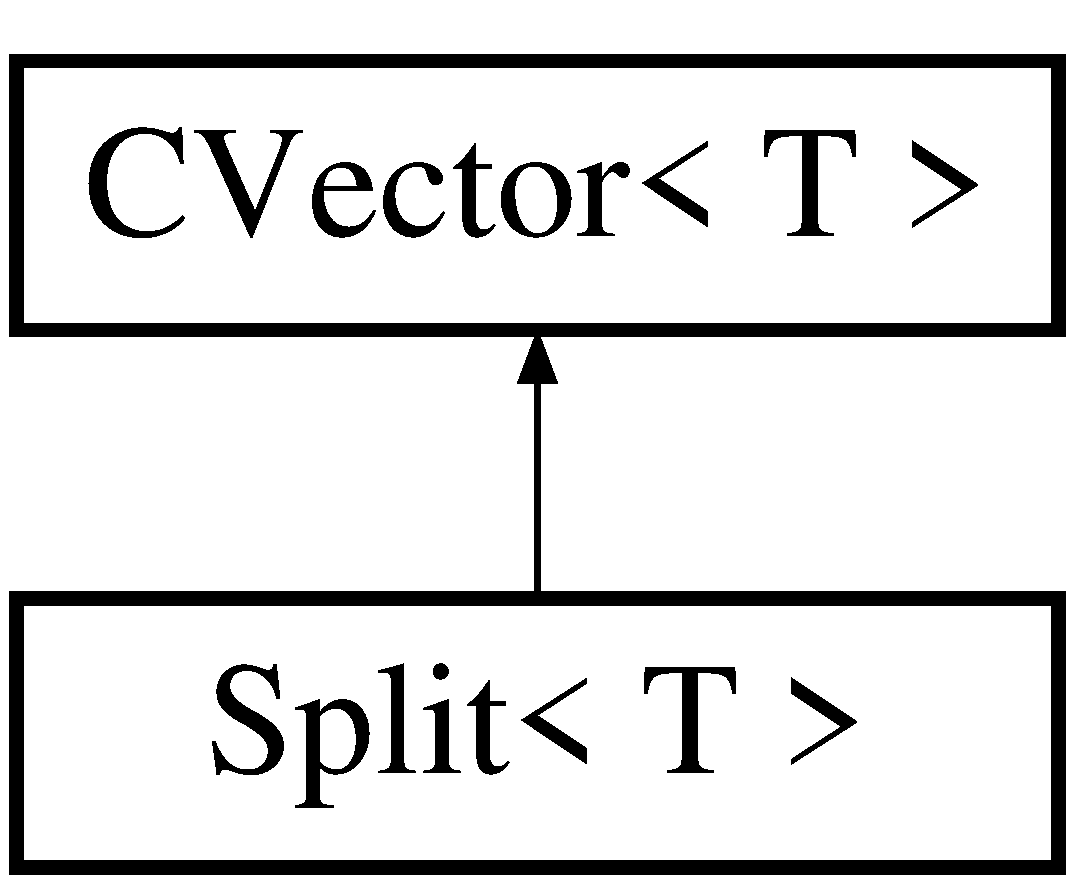
\includegraphics[height=2cm]{classSplit}
\end{center}
\end{figure}
\subsection*{Public Member Functions}
\begin{CompactItemize}
\item 
{\bf Split} ()
\item 
{\bf Split} (size\_\-t)
\item 
bool {\bf operator$<$} (const {\bf Split} \&) const 
\begin{CompactList}\small\item\em whether or not split was flipped \item\end{CompactList}\item 
{\bf Split} ()
\item 
{\bf Split} (size\_\-t)
\item 
bool {\bf operator$<$} (const {\bf Split} \&) const 
\begin{CompactList}\small\item\em starting point of right partition \item\end{CompactList}\end{CompactItemize}
\subsection*{Public Attributes}
\begin{CompactItemize}
\item 
size\_\-t {\bf \_\-rp}
\item 
int {\bf \_\-left}
\begin{CompactList}\small\item\em starting point of right partition \item\end{CompactList}\item 
int {\bf \_\-right}
\begin{CompactList}\small\item\em starting point of right partition \item\end{CompactList}\item 
bool {\bf \_\-flip}
\begin{CompactList}\small\item\em position of split in original tree \item\end{CompactList}\end{CompactItemize}


\subsection{Detailed Description}
\subsubsection*{template$<$class T$>$ class Split$<$ T $>$}

A split corresponds to the bipartition of the leaf set induced by an internal edge. 



\subsection{Constructor \& Destructor Documentation}
\index{Split@{Split}!Split@{Split}}
\index{Split@{Split}!Split@{Split}}
\subsubsection{\setlength{\rightskip}{0pt plus 5cm}template$<$class T$>$ {\bf Split}$<$ T $>$::{\bf Split} ()}\label{classSplit_a0}


\index{Split@{Split}!Split@{Split}}
\index{Split@{Split}!Split@{Split}}
\subsubsection{\setlength{\rightskip}{0pt plus 5cm}template$<$class T$>$ {\bf Split}$<$ T $>$::{\bf Split} (size\_\-t)}\label{classSplit_a1}


\index{Split@{Split}!Split@{Split}}
\index{Split@{Split}!Split@{Split}}
\subsubsection{\setlength{\rightskip}{0pt plus 5cm}template$<$class T$>$ {\bf Split}$<$ T $>$::{\bf Split} ()}\label{classSplit_a3}


\index{Split@{Split}!Split@{Split}}
\index{Split@{Split}!Split@{Split}}
\subsubsection{\setlength{\rightskip}{0pt plus 5cm}template$<$class T$>$ {\bf Split}$<$ T $>$::{\bf Split} (size\_\-t)}\label{classSplit_a4}




\subsection{Member Function Documentation}
\index{Split@{Split}!operator<@{operator$<$}}
\index{operator<@{operator$<$}!Split@{Split}}
\subsubsection{\setlength{\rightskip}{0pt plus 5cm}template$<$class T$>$ bool {\bf Split}$<$ T $>$::operator$<$ (const {\bf Split}$<$ T $>$ \&) const}\label{classSplit_a5}


starting point of right partition 

\index{Split@{Split}!operator<@{operator$<$}}
\index{operator<@{operator$<$}!Split@{Split}}
\subsubsection{\setlength{\rightskip}{0pt plus 5cm}template$<$class T$>$ bool {\bf Split}$<$ T $>$::operator$<$ (const {\bf Split}$<$ T $>$ \&) const}\label{classSplit_a2}


whether or not split was flipped 



\subsection{Member Data Documentation}
\index{Split@{Split}!_flip@{\_\-flip}}
\index{_flip@{\_\-flip}!Split@{Split}}
\subsubsection{\setlength{\rightskip}{0pt plus 5cm}template$<$class T$>$ bool {\bf Split}$<$ T $>$::{\bf \_\-flip}}\label{classSplit_o3}


position of split in original tree 

\index{Split@{Split}!_left@{\_\-left}}
\index{_left@{\_\-left}!Split@{Split}}
\subsubsection{\setlength{\rightskip}{0pt plus 5cm}template$<$class T$>$ int {\bf Split}$<$ T $>$::{\bf \_\-left}}\label{classSplit_o1}


starting point of right partition 

\index{Split@{Split}!_right@{\_\-right}}
\index{_right@{\_\-right}!Split@{Split}}
\subsubsection{\setlength{\rightskip}{0pt plus 5cm}template$<$class T$>$ int {\bf Split}$<$ T $>$::{\bf \_\-right}}\label{classSplit_o2}


starting point of right partition 

\index{Split@{Split}!_rp@{\_\-rp}}
\index{_rp@{\_\-rp}!Split@{Split}}
\subsubsection{\setlength{\rightskip}{0pt plus 5cm}template$<$class T$>$ size\_\-t {\bf Split}$<$ T $>$::{\bf \_\-rp}}\label{classSplit_o0}




The documentation for this class was generated from the following files:\begin{CompactItemize}
\item 
{\bf extractsplitsforest.h}\item 
{\bf splittable.h}\item 
{\bf extractsplitsforest.cpp}\item 
{\bf extractsplitsforest\_\-impl.h}\item 
{\bf splittable\_\-impl.h}\end{CompactItemize}

\section{Split\-PLess$<$ T $>$ Struct Template Reference}
\label{structSplitPLess}\index{SplitPLess@{SplitPLess}}
{\bf Split}{\rm (p.\,\pageref{classSplit})} pointer comparison.  


{\tt \#include $<$extractsplitsforest.h$>$}

\subsection*{Public Member Functions}
\begin{CompactItemize}
\item 
bool {\bf operator()} (const {\bf Split} $\ast$, const {\bf Split} $\ast$) const 
\item 
bool {\bf operator()} ({\bf Split}$<$ T $>$ $\ast$, {\bf Split}$<$ T $>$ $\ast$)
\end{CompactItemize}


\subsection{Detailed Description}
\subsubsection*{template$<$class T$>$ struct Split\-PLess$<$ T $>$}

{\bf Split}{\rm (p.\,\pageref{classSplit})} pointer comparison. 



\subsection{Member Function Documentation}
\index{SplitPLess@{Split\-PLess}!operator()@{operator()}}
\index{operator()@{operator()}!SplitPLess@{Split\-PLess}}
\subsubsection{\setlength{\rightskip}{0pt plus 5cm}template$<$class T$>$ bool {\bf Split\-PLess}$<$ T $>$::operator() ({\bf Split}$<$ T $>$ $\ast$, {\bf Split}$<$ T $>$ $\ast$)}\label{structSplitPLess_a1}


\index{SplitPLess@{Split\-PLess}!operator()@{operator()}}
\index{operator()@{operator()}!SplitPLess@{Split\-PLess}}
\subsubsection{\setlength{\rightskip}{0pt plus 5cm}template$<$class T$>$ bool {\bf Split\-PLess}$<$ T $>$::operator() (const {\bf Split} $\ast$, const {\bf Split} $\ast$) const}\label{structSplitPLess_a0}




The documentation for this struct was generated from the following files:\begin{CompactItemize}
\item 
{\bf extractsplitsforest.h}\item 
{\bf splittable.h}\item 
{\bf extractsplitsforest.cpp}\item 
{\bf splittable\_\-impl.h}\end{CompactItemize}

\section{Split\-Table$<$ T $>$ Class Template Reference}
\label{classSplitTable}\index{SplitTable@{SplitTable}}
The split table can load all non-trivial splits of a tree and provide set-like operations with split tables of other trees in order to identify common splits.  


{\tt \#include $<$splittable.h$>$}

\subsection*{Public Member Functions}
\begin{CompactItemize}
\item 
{\bf Split\-Table} ()
\item 
{\bf Split\-Table} (size\_\-t)
\item 
{\bf $\sim$Split\-Table} ()
\item 
void {\bf resize} (size\_\-t)
\item 
int {\bf get\-Size} () const 
\item 
const {\bf Split}$<$ T $>$ \& {\bf operator[$\,$]} (size\_\-t) const 
\item 
void {\bf load\-Tree} (const {\bf UPTree}$<$ T $>$ \&, const {\bf Bracket\-Table}$<$ T $>$ \&)
\item 
const {\bf Split}$<$ T $>$ $\ast$ {\bf lcs} (const {\bf Split\-Table}$<$ T $>$ \&) const 
\item 
const int {\bf intersection} (const {\bf Split\-Table}$<$ T $>$ \&, {\bf Split\-Table}$<$ T $>$ \&) const 
\end{CompactItemize}
\subsection*{Protected Attributes}
\begin{CompactItemize}
\item 
{\bf CVector}$<$ {\bf Split}$<$ T $>$ $\ast$ $>$ {\bf \_\-splits}
\item 
{\bf Split}$<$ T $>$ {\bf \_\-temp}
\end{CompactItemize}


\subsection{Detailed Description}
\subsubsection*{template$<$class T$>$ class Split\-Table$<$ T $>$}

The split table can load all non-trivial splits of a tree and provide set-like operations with split tables of other trees in order to identify common splits. 

This is a quadratic-sized datastructure with respect to leaf number. 



\subsection{Constructor \& Destructor Documentation}
\index{SplitTable@{Split\-Table}!SplitTable@{SplitTable}}
\index{SplitTable@{SplitTable}!SplitTable@{Split\-Table}}
\subsubsection{\setlength{\rightskip}{0pt plus 5cm}template$<$class T$>$ {\bf Split\-Table}$<$ T $>$::{\bf Split\-Table} ()}\label{classSplitTable_a0}


\index{SplitTable@{Split\-Table}!SplitTable@{SplitTable}}
\index{SplitTable@{SplitTable}!SplitTable@{Split\-Table}}
\subsubsection{\setlength{\rightskip}{0pt plus 5cm}template$<$class T$>$ {\bf Split\-Table}$<$ T $>$::{\bf Split\-Table} (size\_\-t)}\label{classSplitTable_a1}


\index{SplitTable@{Split\-Table}!~SplitTable@{$\sim$SplitTable}}
\index{~SplitTable@{$\sim$SplitTable}!SplitTable@{Split\-Table}}
\subsubsection{\setlength{\rightskip}{0pt plus 5cm}template$<$class T$>$ {\bf Split\-Table}$<$ T $>$::$\sim${\bf Split\-Table} ()}\label{classSplitTable_a2}




\subsection{Member Function Documentation}
\index{SplitTable@{Split\-Table}!getSize@{getSize}}
\index{getSize@{getSize}!SplitTable@{Split\-Table}}
\subsubsection{\setlength{\rightskip}{0pt plus 5cm}template$<$class T$>$ int {\bf Split\-Table}$<$ T $>$::get\-Size () const}\label{classSplitTable_a4}


\index{SplitTable@{Split\-Table}!intersection@{intersection}}
\index{intersection@{intersection}!SplitTable@{Split\-Table}}
\subsubsection{\setlength{\rightskip}{0pt plus 5cm}template$<$class T$>$ const int {\bf Split\-Table}$<$ T $>$::intersection (const {\bf Split\-Table}$<$ T $>$ \&, {\bf Split\-Table}$<$ T $>$ \&) const}\label{classSplitTable_a8}


\index{SplitTable@{Split\-Table}!lcs@{lcs}}
\index{lcs@{lcs}!SplitTable@{Split\-Table}}
\subsubsection{\setlength{\rightskip}{0pt plus 5cm}template$<$class T$>$ const {\bf Split}$<$ T $>$ $\ast$ {\bf Split\-Table}$<$ T $>$::lcs (const {\bf Split\-Table}$<$ T $>$ \&) const}\label{classSplitTable_a7}


\index{SplitTable@{Split\-Table}!loadTree@{loadTree}}
\index{loadTree@{loadTree}!SplitTable@{Split\-Table}}
\subsubsection{\setlength{\rightskip}{0pt plus 5cm}template$<$class T$>$ void {\bf Split\-Table}$<$ T $>$::load\-Tree (const {\bf UPTree}$<$ T $>$ \&, const {\bf Bracket\-Table}$<$ T $>$ \&)}\label{classSplitTable_a6}


\index{SplitTable@{Split\-Table}!operator[]@{operator[]}}
\index{operator[]@{operator[]}!SplitTable@{Split\-Table}}
\subsubsection{\setlength{\rightskip}{0pt plus 5cm}template$<$class T$>$ const {\bf Split}$<$ T $>$ \& {\bf Split\-Table}$<$ T $>$::operator[$\,$] (size\_\-t) const}\label{classSplitTable_a5}


\index{SplitTable@{Split\-Table}!resize@{resize}}
\index{resize@{resize}!SplitTable@{Split\-Table}}
\subsubsection{\setlength{\rightskip}{0pt plus 5cm}template$<$class T$>$ void {\bf Split\-Table}$<$ T $>$::resize (size\_\-t)}\label{classSplitTable_a3}




\subsection{Member Data Documentation}
\index{SplitTable@{Split\-Table}!_splits@{\_\-splits}}
\index{_splits@{\_\-splits}!SplitTable@{Split\-Table}}
\subsubsection{\setlength{\rightskip}{0pt plus 5cm}template$<$class T$>$ {\bf CVector}$<${\bf Split}$<$T$>$$\ast$$>$ {\bf Split\-Table}$<$ T $>$::{\bf \_\-splits}\hspace{0.3cm}{\tt  [protected]}}\label{classSplitTable_p0}


\index{SplitTable@{Split\-Table}!_temp@{\_\-temp}}
\index{_temp@{\_\-temp}!SplitTable@{Split\-Table}}
\subsubsection{\setlength{\rightskip}{0pt plus 5cm}template$<$class T$>$ {\bf Split}$<$T$>$ {\bf Split\-Table}$<$ T $>$::{\bf \_\-temp}\hspace{0.3cm}{\tt  [protected]}}\label{classSplitTable_p1}




The documentation for this class was generated from the following files:\begin{CompactItemize}
\item 
{\bf splittable.h}\item 
{\bf splittable\_\-impl.h}\end{CompactItemize}

\section{Spr\-Helper$<$ T $>$ Class Template Reference}
\label{classSprHelper}\index{SprHelper@{SprHelper}}
Provides quick access to subtrees after a retrifurcation.  


{\tt \#include $<$sprhelper.h$>$}

\subsection*{Public Member Functions}
\begin{CompactItemize}
\item 
{\bf Spr\-Helper} (int)
\item 
{\bf $\sim$Spr\-Helper} ()
\item 
void {\bf flag\-Subtree} (const {\bf UPTree}$<$ T $>$ \&, int, const {\bf Bracket\-Table}$<$ T $>$ \&)
\begin{CompactList}\small\item\em Flag leaf labels of a subtree. \item\end{CompactList}\item 
int {\bf get\-Flagged\-Inverse} (const {\bf UPTree}$<$ T $>$ \&, const {\bf Bracket\-Table}$<$ T $>$ \&)
\end{CompactItemize}
\subsection*{Static Public Member Functions}
\begin{CompactItemize}
\item 
static T {\bf next\-Leaf\-Label} (const {\bf UPTree}$<$ T $>$ \&, int)
\begin{CompactList}\small\item\em Search for the next leaf in the string starting at pos. \item\end{CompactList}\end{CompactItemize}
\subsection*{Protected Attributes}
\begin{CompactItemize}
\item 
bool $\ast$ {\bf \_\-flags}
\item 
int {\bf \_\-size}
\begin{CompactList}\small\item\em leaves corresponding to a subtree are flagged \item\end{CompactList}\end{CompactItemize}
\subsection*{Private Member Functions}
\begin{CompactItemize}
\item 
{\bf Spr\-Helper} ()
\begin{CompactList}\small\item\em tree size (not leaves) \item\end{CompactList}\end{CompactItemize}


\subsection{Detailed Description}
\subsubsection*{template$<$class T$>$ class Spr\-Helper$<$ T $>$}

Provides quick access to subtrees after a retrifurcation. 

Used when enumerating SPR neighbours. 



\subsection{Constructor \& Destructor Documentation}
\index{SprHelper@{Spr\-Helper}!SprHelper@{SprHelper}}
\index{SprHelper@{SprHelper}!SprHelper@{Spr\-Helper}}
\subsubsection{\setlength{\rightskip}{0pt plus 5cm}template$<$class T$>$ {\bf Spr\-Helper}$<$ T $>$::{\bf Spr\-Helper} (int)}\label{classSprHelper_a0}


\index{SprHelper@{Spr\-Helper}!~SprHelper@{$\sim$SprHelper}}
\index{~SprHelper@{$\sim$SprHelper}!SprHelper@{Spr\-Helper}}
\subsubsection{\setlength{\rightskip}{0pt plus 5cm}template$<$class T$>$ {\bf Spr\-Helper}$<$ T $>$::$\sim${\bf Spr\-Helper} ()}\label{classSprHelper_a1}


\index{SprHelper@{Spr\-Helper}!SprHelper@{SprHelper}}
\index{SprHelper@{SprHelper}!SprHelper@{Spr\-Helper}}
\subsubsection{\setlength{\rightskip}{0pt plus 5cm}template$<$class T$>$ {\bf Spr\-Helper}$<$ T $>$::{\bf Spr\-Helper} ()\hspace{0.3cm}{\tt  [private]}}\label{classSprHelper_d0}


tree size (not leaves) 



\subsection{Member Function Documentation}
\index{SprHelper@{Spr\-Helper}!flagSubtree@{flagSubtree}}
\index{flagSubtree@{flagSubtree}!SprHelper@{Spr\-Helper}}
\subsubsection{\setlength{\rightskip}{0pt plus 5cm}template$<$class T$>$ void {\bf Spr\-Helper}$<$ T $>$::flag\-Subtree (const {\bf UPTree}$<$ T $>$ \& {\em tree}, int {\em pos}, const {\bf Bracket\-Table}$<$ T $>$ \& {\em btable})}\label{classSprHelper_a2}


Flag leaf labels of a subtree. 

\begin{Desc}
\item[Parameters:]
\begin{description}
\item[{\em tree}]Input tree. \item[{\em pos}]Start position of the subtree to flag. \item[{\em btable}]Bracket Table associated with the tree. Used to identifiy the end of the subtree. \end{description}
\end{Desc}
\index{SprHelper@{Spr\-Helper}!getFlaggedInverse@{getFlaggedInverse}}
\index{getFlaggedInverse@{getFlaggedInverse}!SprHelper@{Spr\-Helper}}
\subsubsection{\setlength{\rightskip}{0pt plus 5cm}template$<$class T$>$ int {\bf Spr\-Helper}$<$ T $>$::get\-Flagged\-Inverse (const {\bf UPTree}$<$ T $>$ \& {\em tree}, const {\bf Bracket\-Table}$<$ T $>$ \& {\em btable})}\label{classSprHelper_a3}


\begin{Desc}
\item[Returns:]The start position of the subtree corresponding to all the un UNflagged leaves. \end{Desc}
\index{SprHelper@{Spr\-Helper}!nextLeafLabel@{nextLeafLabel}}
\index{nextLeafLabel@{nextLeafLabel}!SprHelper@{Spr\-Helper}}
\subsubsection{\setlength{\rightskip}{0pt plus 5cm}template$<$class T$>$ T {\bf Spr\-Helper}$<$ T $>$::next\-Leaf\-Label (const {\bf UPTree}$<$ T $>$ \& {\em tree}, int {\em pos})\hspace{0.3cm}{\tt  [static]}}\label{classSprHelper_e0}


Search for the next leaf in the string starting at pos. 

Is potentially O(n) so it may be better to search from both ends or use a bracket table or something. 

\subsection{Member Data Documentation}
\index{SprHelper@{Spr\-Helper}!_flags@{\_\-flags}}
\index{_flags@{\_\-flags}!SprHelper@{Spr\-Helper}}
\subsubsection{\setlength{\rightskip}{0pt plus 5cm}template$<$class T$>$ bool$\ast$ {\bf Spr\-Helper}$<$ T $>$::{\bf \_\-flags}\hspace{0.3cm}{\tt  [protected]}}\label{classSprHelper_p0}


\index{SprHelper@{Spr\-Helper}!_size@{\_\-size}}
\index{_size@{\_\-size}!SprHelper@{Spr\-Helper}}
\subsubsection{\setlength{\rightskip}{0pt plus 5cm}template$<$class T$>$ int {\bf Spr\-Helper}$<$ T $>$::{\bf \_\-size}\hspace{0.3cm}{\tt  [protected]}}\label{classSprHelper_p1}


leaves corresponding to a subtree are flagged 



The documentation for this class was generated from the following files:\begin{CompactItemize}
\item 
{\bf sprhelper.h}\item 
{\bf sprhelper\_\-impl.h}\end{CompactItemize}

\section{SPRSearch$<$ T $>$ Class Template Reference}
\label{classSPRSearch}\index{SPRSearch@{SPRSearch}}
Breadth first search of SPR-neighbour graph.  


{\tt \#include $<$sprsearch.h$>$}

\subsection*{Public Types}
\begin{CompactItemize}
\item 
typedef {\bf CVector}$<$ {\bf UPTree}$<$ T $>$ $>$ {\bf Tree\-Pool}
\end{CompactItemize}
\subsection*{Public Member Functions}
\begin{CompactItemize}
\item 
{\bf SPRSearch} ({\bf Tree\-Manager}$<$ T $>$ \&, {\bf Tree\-Cache}$<$ T $>$ \&, unsigned char)
\begin{CompactList}\small\item\em Create an SPR search. \item\end{CompactList}\item 
{\bf $\sim$SPRSearch} ()
\item 
void {\bf set\-Start\-Tree} (const {\bf UPTree}$<$ T $>$ \&)
\begin{CompactList}\small\item\em Add a copy of the start tree to the pool and update the cache. \item\end{CompactList}\item 
void {\bf set\-End\-Tree} (const {\bf UPTree}$<$ T $>$ \&)
\begin{CompactList}\small\item\em Set the end tree. \item\end{CompactList}\item 
bool {\bf iterate} ()
\begin{CompactList}\small\item\em Perform one iteration of the search. \item\end{CompactList}\end{CompactItemize}
\subsection*{Public Attributes}
\begin{CompactItemize}
\item 
size\_\-t {\bf \_\-nni\-Count}
\begin{CompactList}\small\item\em Current iteration. \item\end{CompactList}\item 
size\_\-t {\bf \_\-spr\-Count}
\begin{CompactList}\small\item\em NNI neighbours processed (DEBUG ONLY). \item\end{CompactList}\item 
size\_\-t {\bf \_\-count}
\begin{CompactList}\small\item\em SPR neighbours processed (DEBUG ONLY). \item\end{CompactList}\item 
size\_\-t {\bf \_\-cache\-Hits}
\begin{CompactList}\small\item\em Number of unique trees visited. \item\end{CompactList}\end{CompactItemize}
\subsection*{Protected Member Functions}
\begin{CompactItemize}
\item 
bool {\bf evaluate\-NNI} ({\bf UPTree}$<$ T $>$ \&)
\begin{CompactList}\small\item\em Visit all the (2n-6) NNI neighbours of a tree. \item\end{CompactList}\item 
bool {\bf evaluate\-SPR} ({\bf UPTree}$<$ T $>$ \&)
\begin{CompactList}\small\item\em Visit all the SPR neighbours that ARE NOT NNI neighbours: ie there are at least 2 edges between the cut edge and regraft edge. \item\end{CompactList}\item 
void {\bf swap\-Copy} (const {\bf UPTree}$<$ T $>$ \&, {\bf UPTree}$<$ T $>$ \&, int[2], int[2])
\begin{CompactList}\small\item\em Copies src into dest while swapping the two subtrees corresponding to the ranges specified by sub1 and sub2. \item\end{CompactList}\item 
void {\bf spr\-Copy} (const {\bf UPTree}$<$ T $>$ \&, {\bf UPTree}$<$ T $>$ \&, int, int, const {\bf Bracket\-Table}$<$ T $>$ \&, const {\bf Flag\-Table}$<$ T $>$ \&)
\begin{CompactList}\small\item\em Perform a single spr operation on src tree placing the resulting tree in dest. \item\end{CompactList}\item 
bool {\bf update\-Cache} ({\bf UPTree}$<$ T $>$ \&)
\begin{CompactList}\small\item\em Search for tree in the cache. \item\end{CompactList}\end{CompactItemize}
\subsection*{Protected Attributes}
\begin{CompactItemize}
\item 
{\bf Tree\-Pool} $\ast$ {\bf \_\-pool1}
\item 
{\bf Tree\-Pool} $\ast$ {\bf \_\-pool2}
\begin{CompactList}\small\item\em Unique trees obtained in the previous iteration. \item\end{CompactList}\item 
{\bf Tree\-Pool} {\bf \_\-p1}
\begin{CompactList}\small\item\em Unique trees obtained in the present iteration. \item\end{CompactList}\item 
{\bf Tree\-Pool} {\bf \_\-p2}
\begin{CompactList}\small\item\em A pool of trees. \item\end{CompactList}\item 
{\bf Tree\-Manager}$<$ T $>$ \& {\bf \_\-man}
\begin{CompactList}\small\item\em A pool of trees. \item\end{CompactList}\item 
{\bf Validator}$<$ T $>$ {\bf \_\-valid}
\begin{CompactList}\small\item\em Tree manager used to create new trees. \item\end{CompactList}\item 
{\bf Kernelizor}$<$ T $>$ {\bf \_\-kern}
\begin{CompactList}\small\item\em {\bf Validator}{\rm (p.\,\pageref{classValidator})} used to reorder and retrifurcate. \item\end{CompactList}\item 
{\bf Tree\-Cache}$<$ T $>$ \& {\bf \_\-cache}
\begin{CompactList}\small\item\em {\bf Kernelizor}{\rm (p.\,\pageref{classKernelizor})} used for rekernelization. \item\end{CompactList}\item 
{\bf UPTree}$<$ T $>$ {\bf \_\-spr\-Neighbour}
\begin{CompactList}\small\item\em Tree cache to test for duplicates. \item\end{CompactList}\item 
{\bf UPTree}$<$ T $>$ {\bf \_\-tree\-Buf1}
\begin{CompactList}\small\item\em A reference to the neighbour currently analazyed. \item\end{CompactList}\item 
{\bf UPTree}$<$ T $>$ {\bf \_\-tree\-Buf2}
\begin{CompactList}\small\item\em General purpose temporary tree. \item\end{CompactList}\item 
const {\bf Bracket\-Table}$<$ T $>$ $\ast$ {\bf \_\-btable1}
\begin{CompactList}\small\item\em General purpose tempomrary tree. \item\end{CompactList}\item 
{\bf Bracket\-Table}$<$ T $>$ {\bf \_\-btable2}
\begin{CompactList}\small\item\em Bracket Table of current tree. \item\end{CompactList}\item 
const {\bf Flag\-Table}$<$ T $>$ $\ast$ {\bf \_\-ftable1}
\begin{CompactList}\small\item\em Bracket Table of retrifurcated tree. \item\end{CompactList}\item 
{\bf Flag\-Table}$<$ T $>$ {\bf \_\-ftable2}
\begin{CompactList}\small\item\em Flag Table of current tree. \item\end{CompactList}\item 
{\bf Spr\-Table}$<$ T $>$ {\bf \_\-spr\-Table1}
\begin{CompactList}\small\item\em Flag Table of retrifurcated tree. \item\end{CompactList}\item 
{\bf Spr\-Table}$<$ T $>$ {\bf \_\-spr\-Table2}
\begin{CompactList}\small\item\em SPR edges of current tree. \item\end{CompactList}\item 
{\bf Spr\-Helper}$<$ T $>$ {\bf \_\-spr\-Helper}
\begin{CompactList}\small\item\em SPR edges of retrifurcated tree. \item\end{CompactList}\item 
const int $\ast$ {\bf \_\-lookup1}
\begin{CompactList}\small\item\em Lookup subtrees after retrifurcation. \item\end{CompactList}\item 
unsigned char {\bf \_\-id}
\begin{CompactList}\small\item\em Position - label map forresponding to \_\-btable1. \item\end{CompactList}\item 
short {\bf \_\-iter}
\begin{CompactList}\small\item\em ID of this class. \item\end{CompactList}\end{CompactItemize}
\subsection*{Private Member Functions}
\begin{CompactItemize}
\item 
{\bf SPRSearch} ()
\begin{CompactList}\small\item\em Number of duplicate trees skipped. \item\end{CompactList}\end{CompactItemize}


\subsection{Detailed Description}
\subsubsection*{template$<$class T$>$ class SPRSearch$<$ T $>$}

Breadth first search of SPR-neighbour graph. 

Each tree is checked against a cache. If the tree already exists in the cache, it is ignored unless it has been flagged as an end tree in which case the search terminates. The search works in iterations. Eeach successive call to iterate will evaluate trees of 1 distance greater from the start tree. 



\subsection{Member Typedef Documentation}
\index{SPRSearch@{SPRSearch}!TreePool@{TreePool}}
\index{TreePool@{TreePool}!SPRSearch@{SPRSearch}}
\subsubsection{\setlength{\rightskip}{0pt plus 5cm}template$<$class T$>$ typedef {\bf CVector}$<${\bf UPTree}$<$T$>$ $>$ {\bf SPRSearch}$<$ T $>$::{\bf Tree\-Pool}}\label{classSPRSearch_w0}




\subsection{Constructor \& Destructor Documentation}
\index{SPRSearch@{SPRSearch}!SPRSearch@{SPRSearch}}
\index{SPRSearch@{SPRSearch}!SPRSearch@{SPRSearch}}
\subsubsection{\setlength{\rightskip}{0pt plus 5cm}template$<$class T$>$ {\bf SPRSearch}$<$ T $>$::{\bf SPRSearch} ({\bf Tree\-Manager}$<$ T $>$ \& {\em man}, {\bf Tree\-Cache}$<$ T $>$ \& {\em cache}, unsigned char {\em id})}\label{classSPRSearch_a0}


Create an SPR search. 

Note the default constructor is disabled \begin{Desc}
\item[Parameters:]
\begin{description}
\item[{\em man}]Tree Manager used to create all trees \item[{\em cache}]Tree Cache \end{description}
\end{Desc}
\index{SPRSearch@{SPRSearch}!~SPRSearch@{$\sim$SPRSearch}}
\index{~SPRSearch@{$\sim$SPRSearch}!SPRSearch@{SPRSearch}}
\subsubsection{\setlength{\rightskip}{0pt plus 5cm}template$<$class T$>$ {\bf SPRSearch}$<$ T $>$::$\sim${\bf SPRSearch} ()}\label{classSPRSearch_a1}


\index{SPRSearch@{SPRSearch}!SPRSearch@{SPRSearch}}
\index{SPRSearch@{SPRSearch}!SPRSearch@{SPRSearch}}
\subsubsection{\setlength{\rightskip}{0pt plus 5cm}template$<$class T$>$ {\bf SPRSearch}$<$ T $>$::{\bf SPRSearch} ()\hspace{0.3cm}{\tt  [private]}}\label{classSPRSearch_d0}


Number of duplicate trees skipped. 



\subsection{Member Function Documentation}
\index{SPRSearch@{SPRSearch}!evaluateNNI@{evaluateNNI}}
\index{evaluateNNI@{evaluateNNI}!SPRSearch@{SPRSearch}}
\subsubsection{\setlength{\rightskip}{0pt plus 5cm}template$<$class T$>$ bool {\bf SPRSearch}$<$ T $>$::evaluate\-NNI ({\bf UPTree}$<$ T $>$ \& {\em tree})\hspace{0.3cm}{\tt  [protected]}}\label{classSPRSearch_b0}


Visit all the (2n-6) NNI neighbours of a tree. 

This is a subset of the SPR neighbours and processed separately for counting purposes. (see proof of Theorem 2.1 in Allen and Steel). \index{SPRSearch@{SPRSearch}!evaluateSPR@{evaluateSPR}}
\index{evaluateSPR@{evaluateSPR}!SPRSearch@{SPRSearch}}
\subsubsection{\setlength{\rightskip}{0pt plus 5cm}template$<$class T$>$ bool {\bf SPRSearch}$<$ T $>$::evaluate\-SPR ({\bf UPTree}$<$ T $>$ \& {\em tree})\hspace{0.3cm}{\tt  [protected]}}\label{classSPRSearch_b1}


Visit all the SPR neighbours that ARE NOT NNI neighbours: ie there are at least 2 edges between the cut edge and regraft edge. 

These edges are located with the SPR table. \index{SPRSearch@{SPRSearch}!iterate@{iterate}}
\index{iterate@{iterate}!SPRSearch@{SPRSearch}}
\subsubsection{\setlength{\rightskip}{0pt plus 5cm}template$<$class T$>$ bool {\bf SPRSearch}$<$ T $>$::iterate ()}\label{classSPRSearch_a4}


Perform one iteration of the search. 

All unique neighbours of trees in the current pool are created and added to a pool for the next iteration. Non-unique neighbours are skipped except if their cache flag identifies as an endtree or from a different search, in which case the search terminates. \begin{Desc}
\item[Returns:]true if the search terminates of false otherwise \end{Desc}
\index{SPRSearch@{SPRSearch}!setEndTree@{setEndTree}}
\index{setEndTree@{setEndTree}!SPRSearch@{SPRSearch}}
\subsubsection{\setlength{\rightskip}{0pt plus 5cm}template$<$class T$>$ void {\bf SPRSearch}$<$ T $>$::set\-End\-Tree (const {\bf UPTree}$<$ T $>$ \& {\em t2})}\label{classSPRSearch_a3}


Set the end tree. 

A copy will be used both to check if the search has been completed and for rekernelization at step. \index{SPRSearch@{SPRSearch}!setStartTree@{setStartTree}}
\index{setStartTree@{setStartTree}!SPRSearch@{SPRSearch}}
\subsubsection{\setlength{\rightskip}{0pt plus 5cm}template$<$class T$>$ void {\bf SPRSearch}$<$ T $>$::set\-Start\-Tree (const {\bf UPTree}$<$ T $>$ \& {\em t1})}\label{classSPRSearch_a2}


Add a copy of the start tree to the pool and update the cache. 

\index{SPRSearch@{SPRSearch}!sprCopy@{sprCopy}}
\index{sprCopy@{sprCopy}!SPRSearch@{SPRSearch}}
\subsubsection{\setlength{\rightskip}{0pt plus 5cm}template$<$class T$>$ void {\bf SPRSearch}$<$ T $>$::spr\-Copy (const {\bf UPTree}$<$ T $>$ \& {\em src}, {\bf UPTree}$<$ T $>$ \& {\em dest}, int {\em src\-Pos}, int {\em dest\-Pos}, const {\bf Bracket\-Table}$<$ T $>$ \& {\em btable}, const {\bf Flag\-Table}$<$ T $>$ \& {\em ftable})\hspace{0.3cm}{\tt  [protected]}}\label{classSPRSearch_b3}


Perform a single spr operation on src tree placing the resulting tree in dest. 

\begin{Desc}
\item[Parameters:]
\begin{description}
\item[{\em src}]Source tree \item[{\em dest}]Destination tree \item[{\em src\-Pos}]Position of subtree to prune (in source) \item[{\em dest\-Pos}]Position of subtree to regraft (in source) \item[{\em btable}]Brackettable for source tree. \end{description}
\end{Desc}
\index{SPRSearch@{SPRSearch}!swapCopy@{swapCopy}}
\index{swapCopy@{swapCopy}!SPRSearch@{SPRSearch}}
\subsubsection{\setlength{\rightskip}{0pt plus 5cm}template$<$class T$>$ void {\bf SPRSearch}$<$ T $>$::swap\-Copy (const {\bf UPTree}$<$ T $>$ \& {\em src}, {\bf UPTree}$<$ T $>$ \& {\em dest}, int {\em sub1}[2], int {\em sub2}[2])\hspace{0.3cm}{\tt  [protected]}}\label{classSPRSearch_b2}


Copies src into dest while swapping the two subtrees corresponding to the ranges specified by sub1 and sub2. 

In other words, performs a single NNI operation. \begin{Desc}
\item[Parameters:]
\begin{description}
\item[{\em src}]Source tree \item[{\em dest}]Destination tree \item[{\em sub1}]Positions of first and last elements of subtree to swap with sub2 \item[{\em sub2}]Positions of first and last elements of subtree to swap with sub1 \end{description}
\end{Desc}
\index{SPRSearch@{SPRSearch}!updateCache@{updateCache}}
\index{updateCache@{updateCache}!SPRSearch@{SPRSearch}}
\subsubsection{\setlength{\rightskip}{0pt plus 5cm}template$<$class T$>$ bool {\bf SPRSearch}$<$ T $>$::update\-Cache ({\bf UPTree}$<$ T $>$ \& {\em tree})\hspace{0.3cm}{\tt  [protected]}}\label{classSPRSearch_b4}


Search for tree in the cache. 

If it does not exist, add it to the cache and to the pool for the next iteration. \begin{Desc}
\item[Returns:]true if tree corresponds to the end tree. \end{Desc}


\subsection{Member Data Documentation}
\index{SPRSearch@{SPRSearch}!_btable1@{\_\-btable1}}
\index{_btable1@{\_\-btable1}!SPRSearch@{SPRSearch}}
\subsubsection{\setlength{\rightskip}{0pt plus 5cm}template$<$class T$>$ const {\bf Bracket\-Table}$<$T$>$$\ast$ {\bf SPRSearch}$<$ T $>$::{\bf \_\-btable1}\hspace{0.3cm}{\tt  [protected]}}\label{classSPRSearch_p11}


General purpose tempomrary tree. 

\index{SPRSearch@{SPRSearch}!_btable2@{\_\-btable2}}
\index{_btable2@{\_\-btable2}!SPRSearch@{SPRSearch}}
\subsubsection{\setlength{\rightskip}{0pt plus 5cm}template$<$class T$>$ {\bf Bracket\-Table}$<$T$>$ {\bf SPRSearch}$<$ T $>$::{\bf \_\-btable2}\hspace{0.3cm}{\tt  [protected]}}\label{classSPRSearch_p12}


Bracket Table of current tree. 

\index{SPRSearch@{SPRSearch}!_cache@{\_\-cache}}
\index{_cache@{\_\-cache}!SPRSearch@{SPRSearch}}
\subsubsection{\setlength{\rightskip}{0pt plus 5cm}template$<$class T$>$ {\bf Tree\-Cache}$<$T$>$\& {\bf SPRSearch}$<$ T $>$::{\bf \_\-cache}\hspace{0.3cm}{\tt  [protected]}}\label{classSPRSearch_p7}


{\bf Kernelizor}{\rm (p.\,\pageref{classKernelizor})} used for rekernelization. 

\index{SPRSearch@{SPRSearch}!_cacheHits@{\_\-cacheHits}}
\index{_cacheHits@{\_\-cacheHits}!SPRSearch@{SPRSearch}}
\subsubsection{\setlength{\rightskip}{0pt plus 5cm}template$<$class T$>$ size\_\-t {\bf SPRSearch}$<$ T $>$::{\bf \_\-cache\-Hits}}\label{classSPRSearch_o3}


Number of unique trees visited. 

\index{SPRSearch@{SPRSearch}!_count@{\_\-count}}
\index{_count@{\_\-count}!SPRSearch@{SPRSearch}}
\subsubsection{\setlength{\rightskip}{0pt plus 5cm}template$<$class T$>$ size\_\-t {\bf SPRSearch}$<$ T $>$::{\bf \_\-count}}\label{classSPRSearch_o2}


SPR neighbours processed (DEBUG ONLY). 

\index{SPRSearch@{SPRSearch}!_ftable1@{\_\-ftable1}}
\index{_ftable1@{\_\-ftable1}!SPRSearch@{SPRSearch}}
\subsubsection{\setlength{\rightskip}{0pt plus 5cm}template$<$class T$>$ const {\bf Flag\-Table}$<$T$>$$\ast$ {\bf SPRSearch}$<$ T $>$::{\bf \_\-ftable1}\hspace{0.3cm}{\tt  [protected]}}\label{classSPRSearch_p13}


Bracket Table of retrifurcated tree. 

\index{SPRSearch@{SPRSearch}!_ftable2@{\_\-ftable2}}
\index{_ftable2@{\_\-ftable2}!SPRSearch@{SPRSearch}}
\subsubsection{\setlength{\rightskip}{0pt plus 5cm}template$<$class T$>$ {\bf Flag\-Table}$<$T$>$ {\bf SPRSearch}$<$ T $>$::{\bf \_\-ftable2}\hspace{0.3cm}{\tt  [protected]}}\label{classSPRSearch_p14}


Flag Table of current tree. 

\index{SPRSearch@{SPRSearch}!_id@{\_\-id}}
\index{_id@{\_\-id}!SPRSearch@{SPRSearch}}
\subsubsection{\setlength{\rightskip}{0pt plus 5cm}template$<$class T$>$ unsigned char {\bf SPRSearch}$<$ T $>$::{\bf \_\-id}\hspace{0.3cm}{\tt  [protected]}}\label{classSPRSearch_p19}


Position - label map forresponding to \_\-btable1. 

\index{SPRSearch@{SPRSearch}!_iter@{\_\-iter}}
\index{_iter@{\_\-iter}!SPRSearch@{SPRSearch}}
\subsubsection{\setlength{\rightskip}{0pt plus 5cm}template$<$class T$>$ short {\bf SPRSearch}$<$ T $>$::{\bf \_\-iter}\hspace{0.3cm}{\tt  [protected]}}\label{classSPRSearch_p20}


ID of this class. 

Trees in the cache that do not share this id are considered End trees. (0 or 1) \index{SPRSearch@{SPRSearch}!_kern@{\_\-kern}}
\index{_kern@{\_\-kern}!SPRSearch@{SPRSearch}}
\subsubsection{\setlength{\rightskip}{0pt plus 5cm}template$<$class T$>$ {\bf Kernelizor}$<$T$>$ {\bf SPRSearch}$<$ T $>$::{\bf \_\-kern}\hspace{0.3cm}{\tt  [protected]}}\label{classSPRSearch_p6}


{\bf Validator}{\rm (p.\,\pageref{classValidator})} used to reorder and retrifurcate. 

\index{SPRSearch@{SPRSearch}!_lookup1@{\_\-lookup1}}
\index{_lookup1@{\_\-lookup1}!SPRSearch@{SPRSearch}}
\subsubsection{\setlength{\rightskip}{0pt plus 5cm}template$<$class T$>$ const int$\ast$ {\bf SPRSearch}$<$ T $>$::{\bf \_\-lookup1}\hspace{0.3cm}{\tt  [protected]}}\label{classSPRSearch_p18}


Lookup subtrees after retrifurcation. 

\index{SPRSearch@{SPRSearch}!_man@{\_\-man}}
\index{_man@{\_\-man}!SPRSearch@{SPRSearch}}
\subsubsection{\setlength{\rightskip}{0pt plus 5cm}template$<$class T$>$ {\bf Tree\-Manager}$<$T$>$\& {\bf SPRSearch}$<$ T $>$::{\bf \_\-man}\hspace{0.3cm}{\tt  [protected]}}\label{classSPRSearch_p4}


A pool of trees. 

\index{SPRSearch@{SPRSearch}!_nniCount@{\_\-nniCount}}
\index{_nniCount@{\_\-nniCount}!SPRSearch@{SPRSearch}}
\subsubsection{\setlength{\rightskip}{0pt plus 5cm}template$<$class T$>$ size\_\-t {\bf SPRSearch}$<$ T $>$::{\bf \_\-nni\-Count}}\label{classSPRSearch_o0}


Current iteration. 

\index{SPRSearch@{SPRSearch}!_p1@{\_\-p1}}
\index{_p1@{\_\-p1}!SPRSearch@{SPRSearch}}
\subsubsection{\setlength{\rightskip}{0pt plus 5cm}template$<$class T$>$ {\bf Tree\-Pool} {\bf SPRSearch}$<$ T $>$::{\bf \_\-p1}\hspace{0.3cm}{\tt  [protected]}}\label{classSPRSearch_p2}


Unique trees obtained in the present iteration. 

\index{SPRSearch@{SPRSearch}!_p2@{\_\-p2}}
\index{_p2@{\_\-p2}!SPRSearch@{SPRSearch}}
\subsubsection{\setlength{\rightskip}{0pt plus 5cm}template$<$class T$>$ {\bf Tree\-Pool} {\bf SPRSearch}$<$ T $>$::{\bf \_\-p2}\hspace{0.3cm}{\tt  [protected]}}\label{classSPRSearch_p3}


A pool of trees. 

\index{SPRSearch@{SPRSearch}!_pool1@{\_\-pool1}}
\index{_pool1@{\_\-pool1}!SPRSearch@{SPRSearch}}
\subsubsection{\setlength{\rightskip}{0pt plus 5cm}template$<$class T$>$ {\bf Tree\-Pool}$\ast$ {\bf SPRSearch}$<$ T $>$::{\bf \_\-pool1}\hspace{0.3cm}{\tt  [protected]}}\label{classSPRSearch_p0}


\index{SPRSearch@{SPRSearch}!_pool2@{\_\-pool2}}
\index{_pool2@{\_\-pool2}!SPRSearch@{SPRSearch}}
\subsubsection{\setlength{\rightskip}{0pt plus 5cm}template$<$class T$>$ {\bf Tree\-Pool}$\ast$ {\bf SPRSearch}$<$ T $>$::{\bf \_\-pool2}\hspace{0.3cm}{\tt  [protected]}}\label{classSPRSearch_p1}


Unique trees obtained in the previous iteration. 

\index{SPRSearch@{SPRSearch}!_sprCount@{\_\-sprCount}}
\index{_sprCount@{\_\-sprCount}!SPRSearch@{SPRSearch}}
\subsubsection{\setlength{\rightskip}{0pt plus 5cm}template$<$class T$>$ size\_\-t {\bf SPRSearch}$<$ T $>$::{\bf \_\-spr\-Count}}\label{classSPRSearch_o1}


NNI neighbours processed (DEBUG ONLY). 

\index{SPRSearch@{SPRSearch}!_sprHelper@{\_\-sprHelper}}
\index{_sprHelper@{\_\-sprHelper}!SPRSearch@{SPRSearch}}
\subsubsection{\setlength{\rightskip}{0pt plus 5cm}template$<$class T$>$ {\bf Spr\-Helper}$<$T$>$ {\bf SPRSearch}$<$ T $>$::{\bf \_\-spr\-Helper}\hspace{0.3cm}{\tt  [protected]}}\label{classSPRSearch_p17}


SPR edges of retrifurcated tree. 

\index{SPRSearch@{SPRSearch}!_sprNeighbour@{\_\-sprNeighbour}}
\index{_sprNeighbour@{\_\-sprNeighbour}!SPRSearch@{SPRSearch}}
\subsubsection{\setlength{\rightskip}{0pt plus 5cm}template$<$class T$>$ {\bf UPTree}$<$T$>$ {\bf SPRSearch}$<$ T $>$::{\bf \_\-spr\-Neighbour}\hspace{0.3cm}{\tt  [protected]}}\label{classSPRSearch_p8}


Tree cache to test for duplicates. 

\index{SPRSearch@{SPRSearch}!_sprTable1@{\_\-sprTable1}}
\index{_sprTable1@{\_\-sprTable1}!SPRSearch@{SPRSearch}}
\subsubsection{\setlength{\rightskip}{0pt plus 5cm}template$<$class T$>$ {\bf Spr\-Table}$<$T$>$ {\bf SPRSearch}$<$ T $>$::{\bf \_\-spr\-Table1}\hspace{0.3cm}{\tt  [protected]}}\label{classSPRSearch_p15}


Flag Table of retrifurcated tree. 

\index{SPRSearch@{SPRSearch}!_sprTable2@{\_\-sprTable2}}
\index{_sprTable2@{\_\-sprTable2}!SPRSearch@{SPRSearch}}
\subsubsection{\setlength{\rightskip}{0pt plus 5cm}template$<$class T$>$ {\bf Spr\-Table}$<$T$>$ {\bf SPRSearch}$<$ T $>$::{\bf \_\-spr\-Table2}\hspace{0.3cm}{\tt  [protected]}}\label{classSPRSearch_p16}


SPR edges of current tree. 

\index{SPRSearch@{SPRSearch}!_treeBuf1@{\_\-treeBuf1}}
\index{_treeBuf1@{\_\-treeBuf1}!SPRSearch@{SPRSearch}}
\subsubsection{\setlength{\rightskip}{0pt plus 5cm}template$<$class T$>$ {\bf UPTree}$<$T$>$ {\bf SPRSearch}$<$ T $>$::{\bf \_\-tree\-Buf1}\hspace{0.3cm}{\tt  [protected]}}\label{classSPRSearch_p9}


A reference to the neighbour currently analazyed. 

\index{SPRSearch@{SPRSearch}!_treeBuf2@{\_\-treeBuf2}}
\index{_treeBuf2@{\_\-treeBuf2}!SPRSearch@{SPRSearch}}
\subsubsection{\setlength{\rightskip}{0pt plus 5cm}template$<$class T$>$ {\bf UPTree}$<$T$>$ {\bf SPRSearch}$<$ T $>$::{\bf \_\-tree\-Buf2}\hspace{0.3cm}{\tt  [protected]}}\label{classSPRSearch_p10}


General purpose temporary tree. 

\index{SPRSearch@{SPRSearch}!_valid@{\_\-valid}}
\index{_valid@{\_\-valid}!SPRSearch@{SPRSearch}}
\subsubsection{\setlength{\rightskip}{0pt plus 5cm}template$<$class T$>$ {\bf Validator}$<$T$>$ {\bf SPRSearch}$<$ T $>$::{\bf \_\-valid}\hspace{0.3cm}{\tt  [protected]}}\label{classSPRSearch_p5}


Tree manager used to create new trees. 



The documentation for this class was generated from the following files:\begin{CompactItemize}
\item 
{\bf sprsearch.h}\item 
{\bf sprsearch\_\-impl.h}\end{CompactItemize}

\section{Spr\-Table$<$ T $>$ Class Template Reference}
\label{classSprTable}\index{SprTable@{SprTable}}
Stores all possible regraft points for every subtree in a tree.  


{\tt \#include $<$sprtable.h$>$}

\subsection*{Public Member Functions}
\begin{CompactItemize}
\item 
{\bf Spr\-Table} ()
\item 
{\bf Spr\-Table} (int)
\item 
{\bf $\sim$Spr\-Table} ()
\item 
void {\bf resize} (int)
\begin{CompactList}\small\item\em Resize table if necessary. \item\end{CompactList}\item 
int {\bf load\-Tree} (const {\bf UPTree}$<$ T $>$ \&, const {\bf Bracket\-Table}$<$ T $>$ \&)
\begin{CompactList}\small\item\em Finds the position of all neighbouring subtrees of distance $>$= 2 from each subtree in tree. \item\end{CompactList}\item 
int {\bf load\-Subtree} (const {\bf UPTree}$<$ T $>$ \&, int, const {\bf Bracket\-Table}$<$ T $>$ \&)
\begin{CompactList}\small\item\em Find spr candidate neighbours of all subtrees in a subtree. \item\end{CompactList}\item 
const {\bf NList} $\ast$ {\bf get\-Table} () const 
\begin{CompactList}\small\item\em Get a const pointer to the table. \item\end{CompactList}\item 
const {\bf NList} \& {\bf operator[$\,$]} (int) const 
\begin{CompactList}\small\item\em Get non-NNI spr candidates for a given subtree position. \item\end{CompactList}\end{CompactItemize}
\subsection*{Protected Attributes}
\begin{CompactItemize}
\item 
{\bf NList} $\ast$ {\bf \_\-ntable}
\item 
int {\bf \_\-size}
\begin{CompactList}\small\item\em list of spr neighbours for each subtree \item\end{CompactList}\item 
std::stack$<$ int $>$ {\bf \_\-stack}
\begin{CompactList}\small\item\em size of trees \item\end{CompactList}\end{CompactItemize}
\subsection*{Classes}
\begin{CompactItemize}
\item 
struct {\bf NList}
\begin{CompactList}\small\item\em List of valid regraft points. \item\end{CompactList}\end{CompactItemize}


\subsection{Detailed Description}
\subsubsection*{template$<$class T$>$ class Spr\-Table$<$ T $>$}

Stores all possible regraft points for every subtree in a tree. 

There are O(n) potential points for each subtree (leaf or left bracket) in the tree. NNI's are omitted.

Valid SPR's that are not NNI's are subtrees separated by at least two edges. In the string representation, this corresponds to leaves / left brackets wtih at least 2 unmatched brackets between them. 



\subsection{Constructor \& Destructor Documentation}
\index{SprTable@{Spr\-Table}!SprTable@{SprTable}}
\index{SprTable@{SprTable}!SprTable@{Spr\-Table}}
\subsubsection{\setlength{\rightskip}{0pt plus 5cm}template$<$class T$>$ {\bf Spr\-Table}$<$ T $>$::{\bf Spr\-Table} ()}\label{classSprTable_a0}


\index{SprTable@{Spr\-Table}!SprTable@{SprTable}}
\index{SprTable@{SprTable}!SprTable@{Spr\-Table}}
\subsubsection{\setlength{\rightskip}{0pt plus 5cm}template$<$class T$>$ {\bf Spr\-Table}$<$ T $>$::{\bf Spr\-Table} (int)}\label{classSprTable_a1}


\index{SprTable@{Spr\-Table}!~SprTable@{$\sim$SprTable}}
\index{~SprTable@{$\sim$SprTable}!SprTable@{Spr\-Table}}
\subsubsection{\setlength{\rightskip}{0pt plus 5cm}template$<$class T$>$ {\bf Spr\-Table}$<$ T $>$::$\sim${\bf Spr\-Table} ()}\label{classSprTable_a2}




\subsection{Member Function Documentation}
\index{SprTable@{Spr\-Table}!getTable@{getTable}}
\index{getTable@{getTable}!SprTable@{Spr\-Table}}
\subsubsection{\setlength{\rightskip}{0pt plus 5cm}template$<$class T$>$ const {\bf Spr\-Table}$<$ T $>$::{\bf NList} $\ast$ {\bf Spr\-Table}$<$ T $>$::get\-Table () const\hspace{0.3cm}{\tt  [inline]}}\label{classSprTable_a6}


Get a const pointer to the table. 

\index{SprTable@{Spr\-Table}!loadSubtree@{loadSubtree}}
\index{loadSubtree@{loadSubtree}!SprTable@{Spr\-Table}}
\subsubsection{\setlength{\rightskip}{0pt plus 5cm}template$<$class T$>$ int {\bf Spr\-Table}$<$ T $>$::load\-Subtree (const {\bf UPTree}$<$ T $>$ \& {\em tree}, int {\em pos}, const {\bf Bracket\-Table}$<$ T $>$ \& {\em btable})}\label{classSprTable_a5}


Find spr candidate neighbours of all subtrees in a subtree. 

\index{SprTable@{Spr\-Table}!loadTree@{loadTree}}
\index{loadTree@{loadTree}!SprTable@{Spr\-Table}}
\subsubsection{\setlength{\rightskip}{0pt plus 5cm}template$<$class T$>$ int {\bf Spr\-Table}$<$ T $>$::load\-Tree (const {\bf UPTree}$<$ T $>$ \& {\em tree}, const {\bf Bracket\-Table}$<$ T $>$ \& {\em btable})}\label{classSprTable_a4}


Finds the position of all neighbouring subtrees of distance $>$= 2 from each subtree in tree. 

Very similar to the chain table but we also count subtrees as well as leaves by flagging left-bracket positions. O(n$^\wedge$2) \index{SprTable@{Spr\-Table}!operator[]@{operator[]}}
\index{operator[]@{operator[]}!SprTable@{Spr\-Table}}
\subsubsection{\setlength{\rightskip}{0pt plus 5cm}template$<$class T$>$ const {\bf Spr\-Table}$<$ T $>$::{\bf NList} \& {\bf Spr\-Table}$<$ T $>$::operator[$\,$] (int {\em pos}) const\hspace{0.3cm}{\tt  [inline]}}\label{classSprTable_a7}


Get non-NNI spr candidates for a given subtree position. 

\index{SprTable@{Spr\-Table}!resize@{resize}}
\index{resize@{resize}!SprTable@{Spr\-Table}}
\subsubsection{\setlength{\rightskip}{0pt plus 5cm}template$<$class T$>$ void {\bf Spr\-Table}$<$ T $>$::resize (int {\em size})}\label{classSprTable_a3}


Resize table if necessary. 



\subsection{Member Data Documentation}
\index{SprTable@{Spr\-Table}!_ntable@{\_\-ntable}}
\index{_ntable@{\_\-ntable}!SprTable@{Spr\-Table}}
\subsubsection{\setlength{\rightskip}{0pt plus 5cm}template$<$class T$>$ {\bf NList}$\ast$ {\bf Spr\-Table}$<$ T $>$::{\bf \_\-ntable}\hspace{0.3cm}{\tt  [protected]}}\label{classSprTable_p0}


\index{SprTable@{Spr\-Table}!_size@{\_\-size}}
\index{_size@{\_\-size}!SprTable@{Spr\-Table}}
\subsubsection{\setlength{\rightskip}{0pt plus 5cm}template$<$class T$>$ int {\bf Spr\-Table}$<$ T $>$::{\bf \_\-size}\hspace{0.3cm}{\tt  [protected]}}\label{classSprTable_p1}


list of spr neighbours for each subtree 

\index{SprTable@{Spr\-Table}!_stack@{\_\-stack}}
\index{_stack@{\_\-stack}!SprTable@{Spr\-Table}}
\subsubsection{\setlength{\rightskip}{0pt plus 5cm}template$<$class T$>$ std::stack$<$int$>$ {\bf Spr\-Table}$<$ T $>$::{\bf \_\-stack}\hspace{0.3cm}{\tt  [protected]}}\label{classSprTable_p2}


size of trees 



The documentation for this class was generated from the following files:\begin{CompactItemize}
\item 
{\bf sprtable.h}\item 
{\bf sprtable\_\-impl.h}\end{CompactItemize}

\section{Spr\-Table$<$ T $>$::NList$<$ T $>$ Struct Template Reference}
\label{structSprTable_1_1NList}\index{SprTable::NList@{SprTable::NList}}
List of valid regraft points.  


{\tt \#include $<$sprtable.h$>$}

\subsection*{Public Attributes}
\begin{CompactItemize}
\item 
int {\bf \_\-num}
\item 
int $\ast$ {\bf \_\-pos}
\begin{CompactList}\small\item\em number of neighbours \item\end{CompactList}\end{CompactItemize}


\subsection{Detailed Description}
\subsubsection*{template$<$class T$>$template$<$class T$>$ struct Spr\-Table$<$ T $>$::NList$<$ T $>$}

List of valid regraft points. 



\subsection{Member Data Documentation}
\index{SprTable::NList@{Spr\-Table::NList}!_num@{\_\-num}}
\index{_num@{\_\-num}!SprTable::NList@{Spr\-Table::NList}}
\subsubsection{\setlength{\rightskip}{0pt plus 5cm}template$<$class T$>$ template$<$class T$>$ int {\bf Spr\-Table}$<$ T $>$::{\bf NList}$<$ T $>$::{\bf \_\-num}}\label{structSprTable_1_1NList_o0}


\index{SprTable::NList@{Spr\-Table::NList}!_pos@{\_\-pos}}
\index{_pos@{\_\-pos}!SprTable::NList@{Spr\-Table::NList}}
\subsubsection{\setlength{\rightskip}{0pt plus 5cm}template$<$class T$>$ template$<$class T$>$ int$\ast$ {\bf Spr\-Table}$<$ T $>$::{\bf NList}$<$ T $>$::{\bf \_\-pos}}\label{structSprTable_1_1NList_o1}


number of neighbours 



The documentation for this struct was generated from the following file:\begin{CompactItemize}
\item 
{\bf sprtable.h}\end{CompactItemize}

\section{Subtree\-Rec$<$ T $>$ Struct Template Reference}
\label{structSubtreeRec}\index{SubtreeRec@{SubtreeRec}}
Record corresponding to the information of one subtree.  


{\tt \#include $<$brackettable.h$>$}

\subsection*{Public Attributes}
\begin{CompactItemize}
\item 
T {\bf pos} [2]
\item 
T {\bf r\-Pos}
\begin{CompactList}\small\item\em 0: left 1: right \item\end{CompactList}\item 
T {\bf min} [2]
\begin{CompactList}\small\item\em start of right subtree \item\end{CompactList}\item 
int {\bf state}
\begin{CompactList}\small\item\em 0: left 1: right \item\end{CompactList}\end{CompactItemize}


\subsection{Detailed Description}
\subsubsection*{template$<$class T$>$ struct Subtree\-Rec$<$ T $>$}

Record corresponding to the information of one subtree. 



\subsection{Member Data Documentation}
\index{SubtreeRec@{Subtree\-Rec}!min@{min}}
\index{min@{min}!SubtreeRec@{Subtree\-Rec}}
\subsubsection{\setlength{\rightskip}{0pt plus 5cm}template$<$class T$>$ T {\bf Subtree\-Rec}$<$ T $>$::{\bf min}[2]}\label{structSubtreeRec_o2}


start of right subtree 

\index{SubtreeRec@{Subtree\-Rec}!pos@{pos}}
\index{pos@{pos}!SubtreeRec@{Subtree\-Rec}}
\subsubsection{\setlength{\rightskip}{0pt plus 5cm}template$<$class T$>$ T {\bf Subtree\-Rec}$<$ T $>$::{\bf pos}[2]}\label{structSubtreeRec_o0}


\index{SubtreeRec@{Subtree\-Rec}!rPos@{rPos}}
\index{rPos@{rPos}!SubtreeRec@{Subtree\-Rec}}
\subsubsection{\setlength{\rightskip}{0pt plus 5cm}template$<$class T$>$ T {\bf Subtree\-Rec}$<$ T $>$::{\bf r\-Pos}}\label{structSubtreeRec_o1}


0: left 1: right 

\index{SubtreeRec@{Subtree\-Rec}!state@{state}}
\index{state@{state}!SubtreeRec@{Subtree\-Rec}}
\subsubsection{\setlength{\rightskip}{0pt plus 5cm}template$<$class T$>$ int {\bf Subtree\-Rec}$<$ T $>$::{\bf state}}\label{structSubtreeRec_o3}


0: left 1: right 



The documentation for this struct was generated from the following file:\begin{CompactItemize}
\item 
{\bf brackettable.h}\end{CompactItemize}

\section{Tree\-Cache$<$ T $>$ Class Template Reference}
\label{classTreeCache}\index{TreeCache@{TreeCache}}
Hash table with chaining that stores to references to trees.  


{\tt \#include $<$treecache.h$>$}

\subsection*{Public Member Functions}
\begin{CompactItemize}
\item 
{\bf Tree\-Cache} (size\_\-t, {\bf Tree\-Manager}$<$ T $>$ $\ast$)
\begin{CompactList}\small\item\em Create the cache. \item\end{CompactList}\item 
{\bf $\sim$Tree\-Cache} ()
\item 
void {\bf reset} ()
\begin{CompactList}\small\item\em Remove all elements from the table and reset statistics. \item\end{CompactList}\item 
size\_\-t {\bf size} () const 
\begin{CompactList}\small\item\em Returns the number of elements in the table. \item\end{CompactList}\item 
{\bf Result} {\bf update} (const {\bf UPTree}$<$ T $>$ \&, size\_\-t, size\_\-t)
\begin{CompactList}\small\item\em If the tree exists in the cache, return its flag information. \item\end{CompactList}\item 
{\bf Result} {\bf update} (size\_\-t, size\_\-t, size\_\-t)
\begin{CompactList}\small\item\em If the tree exists in the cache, return its flag information. \item\end{CompactList}\end{CompactItemize}
\subsection*{Public Attributes}
\begin{CompactItemize}
\item 
size\_\-t {\bf \_\-hits}
\begin{CompactList}\small\item\em number of elements stored in \item\end{CompactList}\item 
size\_\-t {\bf \_\-updates}
\begin{CompactList}\small\item\em total cache hits \item\end{CompactList}\item 
size\_\-t {\bf \_\-collisions}
\begin{CompactList}\small\item\em total cache updates \item\end{CompactList}\end{CompactItemize}
\subsection*{Protected Member Functions}
\begin{CompactItemize}
\item 
unsigned int {\bf hash} (size\_\-t)
\begin{CompactList}\small\item\em Hash a tree into an size\_\-t. \item\end{CompactList}\end{CompactItemize}
\subsection*{Protected Attributes}
\begin{CompactItemize}
\item 
{\bf Tree\-Manager}$<$ T $>$ $\ast$ {\bf \_\-man}
\item 
{\bf Node} $\ast$ {\bf \_\-tab}
\begin{CompactList}\small\item\em tree manager where all trees are stored \item\end{CompactList}\item 
size\_\-t {\bf \_\-tab\-Size}
\begin{CompactList}\small\item\em hash table \item\end{CompactList}\item 
size\_\-t {\bf \_\-size}
\begin{CompactList}\small\item\em hash table size (\# buckets) \item\end{CompactList}\end{CompactItemize}
\subsection*{Private Member Functions}
\begin{CompactItemize}
\item 
{\bf Tree\-Cache} ()
\begin{CompactList}\small\item\em total chain collisions \item\end{CompactList}\end{CompactItemize}
\subsection*{Classes}
\begin{CompactItemize}
\item 
struct {\bf Node}
\begin{CompactList}\small\item\em may want to templatize offset? maximum currently iteration hardcoded to 16 ==$>$ maximum distance is 32 os is potentially too small!! TODO: global max os value. \item\end{CompactList}\item 
struct {\bf Result}
\begin{CompactList}\small\item\em {\bf Result}{\rm (p.\,\pageref{structTreeCache_1_1Result})} token for returning status of a call to {\bf update()}{\rm (p.\,\pageref{classTreeCache_a4})}. \item\end{CompactList}\end{CompactItemize}


\subsection{Detailed Description}
\subsubsection*{template$<$class T$>$ class Tree\-Cache$<$ T $>$}

Hash table with chaining that stores to references to trees. 

Each bucket contains a pointer to the tree information in the tree manager as well as a flag denoting which search class the tree was found in. 



\subsection{Constructor \& Destructor Documentation}
\index{TreeCache@{Tree\-Cache}!TreeCache@{TreeCache}}
\index{TreeCache@{TreeCache}!TreeCache@{Tree\-Cache}}
\subsubsection{\setlength{\rightskip}{0pt plus 5cm}template$<$class T$>$ {\bf Tree\-Cache}$<$ T $>$::{\bf Tree\-Cache} (size\_\-t {\em n}, {\bf Tree\-Manager}$<$ T $>$ $\ast$ {\em man})}\label{classTreeCache_a0}


Create the cache. 

\begin{Desc}
\item[Parameters:]
\begin{description}
\item[{\em n}]Size of the table \end{description}
\end{Desc}
\index{TreeCache@{Tree\-Cache}!~TreeCache@{$\sim$TreeCache}}
\index{~TreeCache@{$\sim$TreeCache}!TreeCache@{Tree\-Cache}}
\subsubsection{\setlength{\rightskip}{0pt plus 5cm}template$<$class T$>$ {\bf Tree\-Cache}$<$ T $>$::$\sim${\bf Tree\-Cache} ()}\label{classTreeCache_a1}


\index{TreeCache@{Tree\-Cache}!TreeCache@{TreeCache}}
\index{TreeCache@{TreeCache}!TreeCache@{Tree\-Cache}}
\subsubsection{\setlength{\rightskip}{0pt plus 5cm}template$<$class T$>$ {\bf Tree\-Cache}$<$ T $>$::{\bf Tree\-Cache} ()\hspace{0.3cm}{\tt  [private]}}\label{classTreeCache_d0}


total chain collisions 



\subsection{Member Function Documentation}
\index{TreeCache@{Tree\-Cache}!hash@{hash}}
\index{hash@{hash}!TreeCache@{Tree\-Cache}}
\subsubsection{\setlength{\rightskip}{0pt plus 5cm}template$<$class T$>$ unsigned int {\bf Tree\-Cache}$<$ T $>$::hash (size\_\-t {\em os})\hspace{0.3cm}{\tt  [inline, protected]}}\label{classTreeCache_b0}


Hash a tree into an size\_\-t. 

This is a dumb placeholder function that needs to be replaced. I am currently thinking of crc-32 or a variant. \index{TreeCache@{Tree\-Cache}!reset@{reset}}
\index{reset@{reset}!TreeCache@{Tree\-Cache}}
\subsubsection{\setlength{\rightskip}{0pt plus 5cm}template$<$class T$>$ void {\bf Tree\-Cache}$<$ T $>$::reset ()}\label{classTreeCache_a2}


Remove all elements from the table and reset statistics. 

\index{TreeCache@{Tree\-Cache}!size@{size}}
\index{size@{size}!TreeCache@{Tree\-Cache}}
\subsubsection{\setlength{\rightskip}{0pt plus 5cm}template$<$class T$>$ size\_\-t {\bf Tree\-Cache}$<$ T $>$::size () const\hspace{0.3cm}{\tt  [inline]}}\label{classTreeCache_a3}


Returns the number of elements in the table. 

\index{TreeCache@{Tree\-Cache}!update@{update}}
\index{update@{update}!TreeCache@{Tree\-Cache}}
\subsubsection{\setlength{\rightskip}{0pt plus 5cm}template$<$class T$>$ {\bf Tree\-Cache}$<$ T $>$::{\bf Result} {\bf Tree\-Cache}$<$ T $>$::update (size\_\-t {\em os}, size\_\-t {\em flag}, size\_\-t {\em iter})}\label{classTreeCache_a5}


If the tree exists in the cache, return its flag information. 

Otherwise insert it. \index{TreeCache@{Tree\-Cache}!update@{update}}
\index{update@{update}!TreeCache@{Tree\-Cache}}
\subsubsection{\setlength{\rightskip}{0pt plus 5cm}template$<$class T$>$ {\bf Tree\-Cache}$<$ T $>$::{\bf Result} {\bf Tree\-Cache}$<$ T $>$::update (const {\bf UPTree}$<$ T $>$ \& {\em tree}, size\_\-t {\em flag}, size\_\-t {\em iter})\hspace{0.3cm}{\tt  [inline]}}\label{classTreeCache_a4}


If the tree exists in the cache, return its flag information. 

Otherwise insert it. 

\subsection{Member Data Documentation}
\index{TreeCache@{Tree\-Cache}!_collisions@{\_\-collisions}}
\index{_collisions@{\_\-collisions}!TreeCache@{Tree\-Cache}}
\subsubsection{\setlength{\rightskip}{0pt plus 5cm}template$<$class T$>$ size\_\-t {\bf Tree\-Cache}$<$ T $>$::{\bf \_\-collisions}}\label{classTreeCache_o2}


total cache updates 

\index{TreeCache@{Tree\-Cache}!_hits@{\_\-hits}}
\index{_hits@{\_\-hits}!TreeCache@{Tree\-Cache}}
\subsubsection{\setlength{\rightskip}{0pt plus 5cm}template$<$class T$>$ size\_\-t {\bf Tree\-Cache}$<$ T $>$::{\bf \_\-hits}}\label{classTreeCache_o0}


number of elements stored in 

\index{TreeCache@{Tree\-Cache}!_man@{\_\-man}}
\index{_man@{\_\-man}!TreeCache@{Tree\-Cache}}
\subsubsection{\setlength{\rightskip}{0pt plus 5cm}template$<$class T$>$ {\bf Tree\-Manager}$<$T$>$$\ast$ {\bf Tree\-Cache}$<$ T $>$::{\bf \_\-man}\hspace{0.3cm}{\tt  [protected]}}\label{classTreeCache_p0}


\index{TreeCache@{Tree\-Cache}!_size@{\_\-size}}
\index{_size@{\_\-size}!TreeCache@{Tree\-Cache}}
\subsubsection{\setlength{\rightskip}{0pt plus 5cm}template$<$class T$>$ size\_\-t {\bf Tree\-Cache}$<$ T $>$::{\bf \_\-size}\hspace{0.3cm}{\tt  [protected]}}\label{classTreeCache_p3}


hash table size (\# buckets) 

\index{TreeCache@{Tree\-Cache}!_tab@{\_\-tab}}
\index{_tab@{\_\-tab}!TreeCache@{Tree\-Cache}}
\subsubsection{\setlength{\rightskip}{0pt plus 5cm}template$<$class T$>$ {\bf Node}$\ast$ {\bf Tree\-Cache}$<$ T $>$::{\bf \_\-tab}\hspace{0.3cm}{\tt  [protected]}}\label{classTreeCache_p1}


tree manager where all trees are stored 

\index{TreeCache@{Tree\-Cache}!_tabSize@{\_\-tabSize}}
\index{_tabSize@{\_\-tabSize}!TreeCache@{Tree\-Cache}}
\subsubsection{\setlength{\rightskip}{0pt plus 5cm}template$<$class T$>$ size\_\-t {\bf Tree\-Cache}$<$ T $>$::{\bf \_\-tab\-Size}\hspace{0.3cm}{\tt  [protected]}}\label{classTreeCache_p2}


hash table 

\index{TreeCache@{Tree\-Cache}!_updates@{\_\-updates}}
\index{_updates@{\_\-updates}!TreeCache@{Tree\-Cache}}
\subsubsection{\setlength{\rightskip}{0pt plus 5cm}template$<$class T$>$ size\_\-t {\bf Tree\-Cache}$<$ T $>$::{\bf \_\-updates}}\label{classTreeCache_o1}


total cache hits 



The documentation for this class was generated from the following files:\begin{CompactItemize}
\item 
{\bf treecache.h}\item 
{\bf treecache\_\-impl.h}\end{CompactItemize}

\section{Tree\-Cache$<$ T $>$::Node$<$ T $>$ Struct Template Reference}
\label{structTreeCache_1_1Node}\index{TreeCache::Node@{TreeCache::Node}}
may want to templatize offset? maximum currently iteration hardcoded to 16 ==$>$ maximum distance is 32 os is potentially too small!! TODO: global max os value.  


{\tt \#include $<$treecache.h$>$}

\subsection*{Public Attributes}
\begin{CompactItemize}
\item 
size\_\-t {\bf \_\-os}: sizeof(size\_\-t) $\ast$ 8 - 5
\item 
size\_\-t {\bf \_\-flag}: 1
\begin{CompactList}\small\item\em offset of tree in manager \item\end{CompactList}\item 
size\_\-t {\bf \_\-it}: 4
\begin{CompactList}\small\item\em flag associated with sprsearch object \item\end{CompactList}\item 
{\bf Node} $\ast$ {\bf \_\-next}
\begin{CompactList}\small\item\em is this really necessary??? \item\end{CompactList}\end{CompactItemize}


\subsection{Detailed Description}
\subsubsection*{template$<$class T$>$template$<$class T$>$ struct Tree\-Cache$<$ T $>$::Node$<$ T $>$}

may want to templatize offset? maximum currently iteration hardcoded to 16 ==$>$ maximum distance is 32 os is potentially too small!! TODO: global max os value. 

. some limits need to be generally hardcoded/defined 



\subsection{Member Data Documentation}
\index{TreeCache::Node@{Tree\-Cache::Node}!_flag@{\_\-flag}}
\index{_flag@{\_\-flag}!TreeCache::Node@{Tree\-Cache::Node}}
\subsubsection{\setlength{\rightskip}{0pt plus 5cm}template$<$class T$>$ template$<$class T$>$ size\_\-t {\bf Tree\-Cache}$<$ T $>$::{\bf Node}$<$ T $>$::{\bf \_\-flag}}\label{structTreeCache_1_1Node_o1}


offset of tree in manager 

\index{TreeCache::Node@{Tree\-Cache::Node}!_it@{\_\-it}}
\index{_it@{\_\-it}!TreeCache::Node@{Tree\-Cache::Node}}
\subsubsection{\setlength{\rightskip}{0pt plus 5cm}template$<$class T$>$ template$<$class T$>$ size\_\-t {\bf Tree\-Cache}$<$ T $>$::{\bf Node}$<$ T $>$::{\bf \_\-it}}\label{structTreeCache_1_1Node_o2}


flag associated with sprsearch object 

\index{TreeCache::Node@{Tree\-Cache::Node}!_next@{\_\-next}}
\index{_next@{\_\-next}!TreeCache::Node@{Tree\-Cache::Node}}
\subsubsection{\setlength{\rightskip}{0pt plus 5cm}template$<$class T$>$ template$<$class T$>$ {\bf Node}$\ast$ {\bf Tree\-Cache}$<$ T $>$::{\bf Node}$<$ T $>$::{\bf \_\-next}}\label{structTreeCache_1_1Node_o3}


is this really necessary??? 

\index{TreeCache::Node@{Tree\-Cache::Node}!_os@{\_\-os}}
\index{_os@{\_\-os}!TreeCache::Node@{Tree\-Cache::Node}}
\subsubsection{\setlength{\rightskip}{0pt plus 5cm}template$<$class T$>$ template$<$class T$>$ size\_\-t {\bf Tree\-Cache}$<$ T $>$::{\bf Node}$<$ T $>$::{\bf \_\-os}}\label{structTreeCache_1_1Node_o0}




The documentation for this struct was generated from the following file:\begin{CompactItemize}
\item 
{\bf treecache.h}\end{CompactItemize}

\section{Tree\-Cache$<$ T $>$::Result$<$ T $>$ Struct Template Reference}
\label{structTreeCache_1_1Result}\index{TreeCache::Result@{TreeCache::Result}}
{\bf Result}{\rm (p.\,\pageref{structTreeCache_1_1Result})} token for returning status of a call to {\bf update()}{\rm (p.\,\pageref{classTreeCache_a4})}.  


{\tt \#include $<$treecache.h$>$}

\subsection*{Public Attributes}
\begin{CompactItemize}
\item 
unsigned char {\bf \_\-hit}: 1
\item 
unsigned char {\bf \_\-flag}: 1
\begin{CompactList}\small\item\em denotes whether updated resulted in cache hit \item\end{CompactList}\item 
unsigned char {\bf \_\-it}: 6
\begin{CompactList}\small\item\em if hit == 1, this is the flag of the bucket \item\end{CompactList}\end{CompactItemize}


\subsection{Detailed Description}
\subsubsection*{template$<$class T$>$template$<$class T$>$ struct Tree\-Cache$<$ T $>$::Result$<$ T $>$}

{\bf Result}{\rm (p.\,\pageref{structTreeCache_1_1Result})} token for returning status of a call to {\bf update()}{\rm (p.\,\pageref{classTreeCache_a4})}. 



\subsection{Member Data Documentation}
\index{TreeCache::Result@{Tree\-Cache::Result}!_flag@{\_\-flag}}
\index{_flag@{\_\-flag}!TreeCache::Result@{Tree\-Cache::Result}}
\subsubsection{\setlength{\rightskip}{0pt plus 5cm}template$<$class T$>$ template$<$class T$>$ unsigned char {\bf Tree\-Cache}$<$ T $>$::{\bf Result}$<$ T $>$::{\bf \_\-flag}}\label{structTreeCache_1_1Result_o1}


denotes whether updated resulted in cache hit 

\index{TreeCache::Result@{Tree\-Cache::Result}!_hit@{\_\-hit}}
\index{_hit@{\_\-hit}!TreeCache::Result@{Tree\-Cache::Result}}
\subsubsection{\setlength{\rightskip}{0pt plus 5cm}template$<$class T$>$ template$<$class T$>$ unsigned char {\bf Tree\-Cache}$<$ T $>$::{\bf Result}$<$ T $>$::{\bf \_\-hit}}\label{structTreeCache_1_1Result_o0}


\index{TreeCache::Result@{Tree\-Cache::Result}!_it@{\_\-it}}
\index{_it@{\_\-it}!TreeCache::Result@{Tree\-Cache::Result}}
\subsubsection{\setlength{\rightskip}{0pt plus 5cm}template$<$class T$>$ template$<$class T$>$ unsigned char {\bf Tree\-Cache}$<$ T $>$::{\bf Result}$<$ T $>$::{\bf \_\-it}}\label{structTreeCache_1_1Result_o2}


if hit == 1, this is the flag of the bucket 



The documentation for this struct was generated from the following file:\begin{CompactItemize}
\item 
{\bf treecache.h}\end{CompactItemize}

\section{Tree\-Distance$<$ T $>$ Class Template Reference}
\label{classTreeDistance}\index{TreeDistance@{TreeDistance}}
Compute SPR-distance between two unrooted NEWICK trees.  


{\tt \#include $<$treedistance.h$>$}

\subsection*{Public Member Functions}
\begin{CompactItemize}
\item 
{\bf Tree\-Distance} ()
\item 
{\bf $\sim$Tree\-Distance} ()
\item 
size\_\-t {\bf num\-Leaves} (size\_\-t) const 
\item 
void {\bf set\-Max\-Iterations} (size\_\-t)
\begin{CompactList}\small\item\em Specify maximum number of iterations. \item\end{CompactList}\item 
void {\bf set\-Init\-Manager\-Size} (size\_\-t)
\begin{CompactList}\small\item\em Reset the initial manager size. \item\end{CompactList}\item 
void {\bf set\-Cache\-Table\-Size} (size\_\-t)
\begin{CompactList}\small\item\em Reset the number of buckets in the hash table used by the tree cache as a consequnce, the cache and searchers are out of date. \item\end{CompactList}\item 
bool {\bf set\-Tree} (const std::string \&, int)
\begin{CompactList}\small\item\em Load a Newick tree. \item\end{CompactList}\item 
int {\bf kernelize} ()
\begin{CompactList}\small\item\em Kernelize the two trees loaded with {\bf set\-Tree()}{\rm (p.\,\pageref{classTreeDistance_a6})}. \item\end{CompactList}\item 
int {\bf distance} (bool)
\begin{CompactList}\small\item\em Computes the SPR distance of the trees. \item\end{CompactList}\item 
int {\bf splits\-Forest\-Distance} ()
\item 
int {\bf sync\-Leaf\-Set} ()
\begin{CompactList}\small\item\em This method expects a supertree to be loaded as t1 and and a reference tree (made up of a subset of the supertree's leafset) to be loaded as t2. \item\end{CompactList}\item 
size\_\-t {\bf size} () const 
\item 
size\_\-t {\bf duplicates} () const 
\end{CompactItemize}
\subsection*{Protected Member Functions}
\begin{CompactItemize}
\item 
void {\bf init\-Kernelize\-Structures} ()
\begin{CompactList}\small\item\em Ensure that all kernelization structures are properly allocated for the current tree size. \item\end{CompactList}\item 
void {\bf init\-Search\-Structures} ()
\begin{CompactList}\small\item\em Ensure that all search sutructures are properly allocated for the current tree size. \item\end{CompactList}\item 
void {\bf init\-Leaf\-Set\-Structures} ()
\begin{CompactList}\small\item\em Ensure that all structures required for supertree extraction are properly allocated for the current tree size. \item\end{CompactList}\end{CompactItemize}
\subsection*{Protected Attributes}
\begin{CompactItemize}
\item 
std::vector$<$ std::string $>$ {\bf \_\-name\-Lookup} [2]
\item 
std::string {\bf \_\-tree\-String} [2]
\begin{CompactList}\small\item\em maps leaf names to numbers \item\end{CompactList}\item 
size\_\-t {\bf \_\-num\-Leaves\-Kernelized}
\begin{CompactList}\small\item\em copy of input tree strings \item\end{CompactList}\item 
size\_\-t {\bf \_\-max\-Iterations}
\begin{CompactList}\small\item\em \# leaves in kernelized trees \item\end{CompactList}\item 
size\_\-t {\bf \_\-cache\-Table\-Size}
\begin{CompactList}\small\item\em max iterations for search \item\end{CompactList}\item 
size\_\-t {\bf \_\-init\-Manager\-Size}
\begin{CompactList}\small\item\em size of hash table array \item\end{CompactList}\item 
size\_\-t {\bf \_\-num\-Trees\-Searched}
\begin{CompactList}\small\item\em size of inital alloc of treemanager \item\end{CompactList}\item 
size\_\-t {\bf \_\-num\-Cache\-Hits}
\item 
{\bf Tree\-Manager}$<$ unsigned short $>$ $\ast$ {\bf \_\-big\-Manager}
\item 
{\bf Tree\-Manager}$<$ unsigned short $>$ $\ast$ {\bf \_\-big\-Manager2}
\begin{CompactList}\small\item\em manager for 16-bit trees \item\end{CompactList}\item 
{\bf Kernelizor}$<$ unsigned short $>$ $\ast$ {\bf \_\-big\-Kernelizor}
\begin{CompactList}\small\item\em manager for 16-bit trees \item\end{CompactList}\item 
{\bf Validator}$<$ unsigned short $>$ $\ast$ {\bf \_\-big\-Validator}
\begin{CompactList}\small\item\em kernelizor for 16-bit trees \item\end{CompactList}\item 
{\bf Extract\-Subtree}$<$ unsigned short, unsigned short $>$ {\bf \_\-big\-Extractor}
\begin{CompactList}\small\item\em validator for 16-bit trees \item\end{CompactList}\item 
{\bf Extract\-Splits\-Forest} {\bf \_\-splits\-Forest}
\begin{CompactList}\small\item\em support for supertree extraction \item\end{CompactList}\item 
{\bf Tree\-Manager}$<$ unsigned char $>$ $\ast$ {\bf \_\-manager}
\begin{CompactList}\small\item\em support for splits heuristic \item\end{CompactList}\item 
{\bf Tree\-Cache}$<$ unsigned char $>$ $\ast$ {\bf \_\-cache}
\begin{CompactList}\small\item\em byte tree manager \item\end{CompactList}\item 
{\bf Validator}$<$ unsigned char $>$ $\ast$ {\bf \_\-validator}
\begin{CompactList}\small\item\em byte tree cache \item\end{CompactList}\item 
{\bf SPRSearch}$<$ unsigned char $>$ $\ast$ {\bf \_\-searcher} [2]
\begin{CompactList}\small\item\em byte tree validator \item\end{CompactList}\end{CompactItemize}


\subsection{Detailed Description}
\subsubsection*{template$<$class T$>$ class Tree\-Distance$<$ T $>$}

Compute SPR-distance between two unrooted NEWICK trees. 

This class presently takes as input any pair of unrooted trees with the same leaf set where the number of leaves is less than 2$^\wedge$13 - 1. The SPR distance is computed by first kernelizing the input trees then performing two exhaustive breadth first searches, one beginning at each tree. A minimal SPR-distance is obtained when both searches reach a common topolgy.

BUG: I don't think {\bf distance()}{\rm (p.\,\pageref{classTreeDistance_a8})} currently works without {\bf kernelize()}{\rm (p.\,\pageref{classTreeDistance_a7})} being called first because numleaveskernelized is required... 



\subsection{Constructor \& Destructor Documentation}
\index{TreeDistance@{Tree\-Distance}!TreeDistance@{TreeDistance}}
\index{TreeDistance@{TreeDistance}!TreeDistance@{Tree\-Distance}}
\subsubsection{\setlength{\rightskip}{0pt plus 5cm}template$<$class T$>$ {\bf Tree\-Distance}$<$ T $>$::{\bf Tree\-Distance} ()}\label{classTreeDistance_a0}


\index{TreeDistance@{Tree\-Distance}!~TreeDistance@{$\sim$TreeDistance}}
\index{~TreeDistance@{$\sim$TreeDistance}!TreeDistance@{Tree\-Distance}}
\subsubsection{\setlength{\rightskip}{0pt plus 5cm}template$<$class T$>$ {\bf Tree\-Distance}$<$ T $>$::$\sim${\bf Tree\-Distance} ()}\label{classTreeDistance_a1}




\subsection{Member Function Documentation}
\index{TreeDistance@{Tree\-Distance}!distance@{distance}}
\index{distance@{distance}!TreeDistance@{Tree\-Distance}}
\subsubsection{\setlength{\rightskip}{0pt plus 5cm}template$<$class T$>$ int {\bf Tree\-Distance}$<$ T $>$::distance (bool {\em use\-Split\-Forest})}\label{classTreeDistance_a8}


Computes the SPR distance of the trees. 

\begin{Desc}
\item[Returns:]Distance if success, -1 otherwise. \end{Desc}
\index{TreeDistance@{Tree\-Distance}!duplicates@{duplicates}}
\index{duplicates@{duplicates}!TreeDistance@{Tree\-Distance}}
\subsubsection{\setlength{\rightskip}{0pt plus 5cm}template$<$class T$>$ size\_\-t {\bf Tree\-Distance}$<$ T $>$::duplicates () const}\label{classTreeDistance_a12}


\index{TreeDistance@{Tree\-Distance}!initKernelizeStructures@{initKernelizeStructures}}
\index{initKernelizeStructures@{initKernelizeStructures}!TreeDistance@{Tree\-Distance}}
\subsubsection{\setlength{\rightskip}{0pt plus 5cm}template$<$class T$>$ void {\bf Tree\-Distance}$<$ T $>$::init\-Kernelize\-Structures ()\hspace{0.3cm}{\tt  [protected]}}\label{classTreeDistance_b0}


Ensure that all kernelization structures are properly allocated for the current tree size. 

\index{TreeDistance@{Tree\-Distance}!initLeafSetStructures@{initLeafSetStructures}}
\index{initLeafSetStructures@{initLeafSetStructures}!TreeDistance@{Tree\-Distance}}
\subsubsection{\setlength{\rightskip}{0pt plus 5cm}template$<$class T$>$ void {\bf Tree\-Distance}$<$ T $>$::init\-Leaf\-Set\-Structures ()\hspace{0.3cm}{\tt  [protected]}}\label{classTreeDistance_b2}


Ensure that all structures required for supertree extraction are properly allocated for the current tree size. 

\index{TreeDistance@{Tree\-Distance}!initSearchStructures@{initSearchStructures}}
\index{initSearchStructures@{initSearchStructures}!TreeDistance@{Tree\-Distance}}
\subsubsection{\setlength{\rightskip}{0pt plus 5cm}template$<$class T$>$ void {\bf Tree\-Distance}$<$ T $>$::init\-Search\-Structures ()\hspace{0.3cm}{\tt  [protected]}}\label{classTreeDistance_b1}


Ensure that all search sutructures are properly allocated for the current tree size. 

\index{TreeDistance@{Tree\-Distance}!kernelize@{kernelize}}
\index{kernelize@{kernelize}!TreeDistance@{Tree\-Distance}}
\subsubsection{\setlength{\rightskip}{0pt plus 5cm}template$<$class T$>$ int {\bf Tree\-Distance}$<$ T $>$::kernelize ()}\label{classTreeDistance_a7}


Kernelize the two trees loaded with {\bf set\-Tree()}{\rm (p.\,\pageref{classTreeDistance_a6})}. 

\begin{Desc}
\item[Returns:]Number of leaves removed by kernelization. \end{Desc}
\index{TreeDistance@{Tree\-Distance}!numLeaves@{numLeaves}}
\index{numLeaves@{numLeaves}!TreeDistance@{Tree\-Distance}}
\subsubsection{\setlength{\rightskip}{0pt plus 5cm}template$<$class T$>$ size\_\-t {\bf Tree\-Distance}$<$ T $>$::num\-Leaves (size\_\-t) const}\label{classTreeDistance_a2}


\index{TreeDistance@{Tree\-Distance}!setCacheTableSize@{setCacheTableSize}}
\index{setCacheTableSize@{setCacheTableSize}!TreeDistance@{Tree\-Distance}}
\subsubsection{\setlength{\rightskip}{0pt plus 5cm}template$<$class T$>$ void {\bf Tree\-Distance}$<$ T $>$::set\-Cache\-Table\-Size (size\_\-t {\em size})}\label{classTreeDistance_a5}


Reset the number of buckets in the hash table used by the tree cache as a consequnce, the cache and searchers are out of date. 

\index{TreeDistance@{Tree\-Distance}!setInitManagerSize@{setInitManagerSize}}
\index{setInitManagerSize@{setInitManagerSize}!TreeDistance@{Tree\-Distance}}
\subsubsection{\setlength{\rightskip}{0pt plus 5cm}template$<$class T$>$ void {\bf Tree\-Distance}$<$ T $>$::set\-Init\-Manager\-Size (size\_\-t {\em size})}\label{classTreeDistance_a4}


Reset the initial manager size. 

as a consequence, the other structures must also be hosed. i can't really think of a reason why this function woudl be useful. \index{TreeDistance@{Tree\-Distance}!setMaxIterations@{setMaxIterations}}
\index{setMaxIterations@{setMaxIterations}!TreeDistance@{Tree\-Distance}}
\subsubsection{\setlength{\rightskip}{0pt plus 5cm}template$<$class T$>$ void {\bf Tree\-Distance}$<$ T $>$::set\-Max\-Iterations (size\_\-t {\em mi})}\label{classTreeDistance_a3}


Specify maximum number of iterations. 

\index{TreeDistance@{Tree\-Distance}!setTree@{setTree}}
\index{setTree@{setTree}!TreeDistance@{Tree\-Distance}}
\subsubsection{\setlength{\rightskip}{0pt plus 5cm}template$<$class T$>$ bool {\bf Tree\-Distance}$<$ T $>$::set\-Tree (const std::string \& {\em in\-String}, int {\em num})}\label{classTreeDistance_a6}


Load a Newick tree. 

\begin{Desc}
\item[Parameters:]
\begin{description}
\item[{\em num}]Specify T1 or T2 (must be 0 or 1) \end{description}
\end{Desc}
\begin{Desc}
\item[Returns:]true if successfully loaded, false otherwise \end{Desc}
\index{TreeDistance@{Tree\-Distance}!size@{size}}
\index{size@{size}!TreeDistance@{Tree\-Distance}}
\subsubsection{\setlength{\rightskip}{0pt plus 5cm}template$<$class T$>$ size\_\-t {\bf Tree\-Distance}$<$ T $>$::size () const}\label{classTreeDistance_a11}


\begin{Desc}
\item[Returns:]the number of trees in memory. this is the size of the last search performed. \end{Desc}
\index{TreeDistance@{Tree\-Distance}!splitsForestDistance@{splitsForestDistance}}
\index{splitsForestDistance@{splitsForestDistance}!TreeDistance@{Tree\-Distance}}
\subsubsection{\setlength{\rightskip}{0pt plus 5cm}template$<$class T$>$ int {\bf Tree\-Distance}$<$ T $>$::splits\-Forest\-Distance ()}\label{classTreeDistance_a9}


\index{TreeDistance@{Tree\-Distance}!syncLeafSet@{syncLeafSet}}
\index{syncLeafSet@{syncLeafSet}!TreeDistance@{Tree\-Distance}}
\subsubsection{\setlength{\rightskip}{0pt plus 5cm}template$<$class T$>$ int {\bf Tree\-Distance}$<$ T $>$::sync\-Leaf\-Set ()}\label{classTreeDistance_a10}


This method expects a supertree to be loaded as t1 and and a reference tree (made up of a subset of the supertree's leafset) to be loaded as t2. 

All leaves of the supertree notin the reference tree will be removed so that t1 and t2 are of the same size and comparable by the SPR distance metric. \begin{Desc}
\item[Returns:]0 is operation was successful. \end{Desc}


\subsection{Member Data Documentation}
\index{TreeDistance@{Tree\-Distance}!_bigExtractor@{\_\-bigExtractor}}
\index{_bigExtractor@{\_\-bigExtractor}!TreeDistance@{Tree\-Distance}}
\subsubsection{\setlength{\rightskip}{0pt plus 5cm}template$<$class T$>$ {\bf Extract\-Subtree}$<$unsigned short, unsigned short$>$ {\bf Tree\-Distance}$<$ T $>$::{\bf \_\-big\-Extractor}\hspace{0.3cm}{\tt  [protected]}}\label{classTreeDistance_p12}


validator for 16-bit trees 

\index{TreeDistance@{Tree\-Distance}!_bigKernelizor@{\_\-bigKernelizor}}
\index{_bigKernelizor@{\_\-bigKernelizor}!TreeDistance@{Tree\-Distance}}
\subsubsection{\setlength{\rightskip}{0pt plus 5cm}template$<$class T$>$ {\bf Kernelizor}$<$unsigned short$>$$\ast$ {\bf Tree\-Distance}$<$ T $>$::{\bf \_\-big\-Kernelizor}\hspace{0.3cm}{\tt  [protected]}}\label{classTreeDistance_p10}


manager for 16-bit trees 

\index{TreeDistance@{Tree\-Distance}!_bigManager@{\_\-bigManager}}
\index{_bigManager@{\_\-bigManager}!TreeDistance@{Tree\-Distance}}
\subsubsection{\setlength{\rightskip}{0pt plus 5cm}template$<$class T$>$ {\bf Tree\-Manager}$<$unsigned short$>$$\ast$ {\bf Tree\-Distance}$<$ T $>$::{\bf \_\-big\-Manager}\hspace{0.3cm}{\tt  [protected]}}\label{classTreeDistance_p8}


\index{TreeDistance@{Tree\-Distance}!_bigManager2@{\_\-bigManager2}}
\index{_bigManager2@{\_\-bigManager2}!TreeDistance@{Tree\-Distance}}
\subsubsection{\setlength{\rightskip}{0pt plus 5cm}template$<$class T$>$ {\bf Tree\-Manager}$<$unsigned short$>$$\ast$ {\bf Tree\-Distance}$<$ T $>$::{\bf \_\-big\-Manager2}\hspace{0.3cm}{\tt  [protected]}}\label{classTreeDistance_p9}


manager for 16-bit trees 

\index{TreeDistance@{Tree\-Distance}!_bigValidator@{\_\-bigValidator}}
\index{_bigValidator@{\_\-bigValidator}!TreeDistance@{Tree\-Distance}}
\subsubsection{\setlength{\rightskip}{0pt plus 5cm}template$<$class T$>$ {\bf Validator}$<$unsigned short$>$$\ast$ {\bf Tree\-Distance}$<$ T $>$::{\bf \_\-big\-Validator}\hspace{0.3cm}{\tt  [protected]}}\label{classTreeDistance_p11}


kernelizor for 16-bit trees 

\index{TreeDistance@{Tree\-Distance}!_cache@{\_\-cache}}
\index{_cache@{\_\-cache}!TreeDistance@{Tree\-Distance}}
\subsubsection{\setlength{\rightskip}{0pt plus 5cm}template$<$class T$>$ {\bf Tree\-Cache}$<$unsigned char$>$$\ast$ {\bf Tree\-Distance}$<$ T $>$::{\bf \_\-cache}\hspace{0.3cm}{\tt  [protected]}}\label{classTreeDistance_p15}


byte tree manager 

\index{TreeDistance@{Tree\-Distance}!_cacheTableSize@{\_\-cacheTableSize}}
\index{_cacheTableSize@{\_\-cacheTableSize}!TreeDistance@{Tree\-Distance}}
\subsubsection{\setlength{\rightskip}{0pt plus 5cm}template$<$class T$>$ size\_\-t {\bf Tree\-Distance}$<$ T $>$::{\bf \_\-cache\-Table\-Size}\hspace{0.3cm}{\tt  [protected]}}\label{classTreeDistance_p4}


max iterations for search 

\index{TreeDistance@{Tree\-Distance}!_initManagerSize@{\_\-initManagerSize}}
\index{_initManagerSize@{\_\-initManagerSize}!TreeDistance@{Tree\-Distance}}
\subsubsection{\setlength{\rightskip}{0pt plus 5cm}template$<$class T$>$ size\_\-t {\bf Tree\-Distance}$<$ T $>$::{\bf \_\-init\-Manager\-Size}\hspace{0.3cm}{\tt  [protected]}}\label{classTreeDistance_p5}


size of hash table array 

\index{TreeDistance@{Tree\-Distance}!_manager@{\_\-manager}}
\index{_manager@{\_\-manager}!TreeDistance@{Tree\-Distance}}
\subsubsection{\setlength{\rightskip}{0pt plus 5cm}template$<$class T$>$ {\bf Tree\-Manager}$<$unsigned char$>$$\ast$ {\bf Tree\-Distance}$<$ T $>$::{\bf \_\-manager}\hspace{0.3cm}{\tt  [protected]}}\label{classTreeDistance_p14}


support for splits heuristic 

\index{TreeDistance@{Tree\-Distance}!_maxIterations@{\_\-maxIterations}}
\index{_maxIterations@{\_\-maxIterations}!TreeDistance@{Tree\-Distance}}
\subsubsection{\setlength{\rightskip}{0pt plus 5cm}template$<$class T$>$ size\_\-t {\bf Tree\-Distance}$<$ T $>$::{\bf \_\-max\-Iterations}\hspace{0.3cm}{\tt  [protected]}}\label{classTreeDistance_p3}


\# leaves in kernelized trees 

\index{TreeDistance@{Tree\-Distance}!_nameLookup@{\_\-nameLookup}}
\index{_nameLookup@{\_\-nameLookup}!TreeDistance@{Tree\-Distance}}
\subsubsection{\setlength{\rightskip}{0pt plus 5cm}template$<$class T$>$ std::vector$<$std::string$>$ {\bf Tree\-Distance}$<$ T $>$::{\bf \_\-name\-Lookup}[2]\hspace{0.3cm}{\tt  [protected]}}\label{classTreeDistance_p0}


\index{TreeDistance@{Tree\-Distance}!_numCacheHits@{\_\-numCacheHits}}
\index{_numCacheHits@{\_\-numCacheHits}!TreeDistance@{Tree\-Distance}}
\subsubsection{\setlength{\rightskip}{0pt plus 5cm}template$<$class T$>$ size\_\-t {\bf Tree\-Distance}$<$ T $>$::{\bf \_\-num\-Cache\-Hits}\hspace{0.3cm}{\tt  [protected]}}\label{classTreeDistance_p7}


\index{TreeDistance@{Tree\-Distance}!_numLeavesKernelized@{\_\-numLeavesKernelized}}
\index{_numLeavesKernelized@{\_\-numLeavesKernelized}!TreeDistance@{Tree\-Distance}}
\subsubsection{\setlength{\rightskip}{0pt plus 5cm}template$<$class T$>$ size\_\-t {\bf Tree\-Distance}$<$ T $>$::{\bf \_\-num\-Leaves\-Kernelized}\hspace{0.3cm}{\tt  [protected]}}\label{classTreeDistance_p2}


copy of input tree strings 

\index{TreeDistance@{Tree\-Distance}!_numTreesSearched@{\_\-numTreesSearched}}
\index{_numTreesSearched@{\_\-numTreesSearched}!TreeDistance@{Tree\-Distance}}
\subsubsection{\setlength{\rightskip}{0pt plus 5cm}template$<$class T$>$ size\_\-t {\bf Tree\-Distance}$<$ T $>$::{\bf \_\-num\-Trees\-Searched}\hspace{0.3cm}{\tt  [protected]}}\label{classTreeDistance_p6}


size of inital alloc of treemanager 

\index{TreeDistance@{Tree\-Distance}!_searcher@{\_\-searcher}}
\index{_searcher@{\_\-searcher}!TreeDistance@{Tree\-Distance}}
\subsubsection{\setlength{\rightskip}{0pt plus 5cm}template$<$class T$>$ {\bf SPRSearch}$<$unsigned char$>$$\ast$ {\bf Tree\-Distance}$<$ T $>$::{\bf \_\-searcher}[2]\hspace{0.3cm}{\tt  [protected]}}\label{classTreeDistance_p17}


byte tree validator 

\index{TreeDistance@{Tree\-Distance}!_splitsForest@{\_\-splitsForest}}
\index{_splitsForest@{\_\-splitsForest}!TreeDistance@{Tree\-Distance}}
\subsubsection{\setlength{\rightskip}{0pt plus 5cm}template$<$class T$>$ {\bf Extract\-Splits\-Forest} {\bf Tree\-Distance}$<$ T $>$::{\bf \_\-splits\-Forest}\hspace{0.3cm}{\tt  [protected]}}\label{classTreeDistance_p13}


support for supertree extraction 

\index{TreeDistance@{Tree\-Distance}!_treeString@{\_\-treeString}}
\index{_treeString@{\_\-treeString}!TreeDistance@{Tree\-Distance}}
\subsubsection{\setlength{\rightskip}{0pt plus 5cm}template$<$class T$>$ std::string {\bf Tree\-Distance}$<$ T $>$::{\bf \_\-tree\-String}[2]\hspace{0.3cm}{\tt  [protected]}}\label{classTreeDistance_p1}


maps leaf names to numbers 

\index{TreeDistance@{Tree\-Distance}!_validator@{\_\-validator}}
\index{_validator@{\_\-validator}!TreeDistance@{Tree\-Distance}}
\subsubsection{\setlength{\rightskip}{0pt plus 5cm}template$<$class T$>$ {\bf Validator}$<$unsigned char$>$$\ast$ {\bf Tree\-Distance}$<$ T $>$::{\bf \_\-validator}\hspace{0.3cm}{\tt  [protected]}}\label{classTreeDistance_p16}


byte tree cache 



The documentation for this class was generated from the following files:\begin{CompactItemize}
\item 
{\bf treedistance.h}\item 
{\bf treedistance.cpp}\end{CompactItemize}

\section{Tree\-Manager$<$ T $>$ Class Template Reference}
\label{classTreeManager}\index{TreeManager@{TreeManager}}
Stores a given number of trees in a contiguous chunk of memory.  


{\tt \#include $<$treemanager.h$>$}

\subsection*{Public Member Functions}
\begin{CompactItemize}
\item 
{\bf Tree\-Manager} (size\_\-t, size\_\-t)
\item 
{\bf $\sim$Tree\-Manager} ()
\item 
{\bf Tree\-Tok}$<$ T $>$ {\bf operator[$\,$]} (size\_\-t) const 
\item 
{\bf Tree\-Tok}$<$ T $>$ \& {\bf operator[$\,$]} (size\_\-t)
\item 
size\_\-t {\bf tree\-Size} () const 
\item 
size\_\-t {\bf num\-Leaves} () const 
\item 
size\_\-t {\bf size} () const 
\item 
void {\bf reset} ()
\begin{CompactList}\small\item\em Erase all the trees (but don't deallocate). \item\end{CompactList}\item 
void {\bf create\-Tree} ({\bf UPTree}$<$ T $>$ \&)
\begin{CompactList}\small\item\em Creates a new tree and reserves the appropriate memory, resizing if the capacity is exceeded  Output tree. \item\end{CompactList}\item 
void {\bf get\-Tree} (size\_\-t, {\bf UPTree}$<$ T $>$ \&)
\begin{CompactList}\small\item\em Request a tree at a given offset and update tree to point to it. \item\end{CompactList}\item 
void {\bf delete\-Last} ()
\begin{CompactList}\small\item\em Delete (unrserve space corresponding to) the tree most recently created with {\bf create\-Tree()}{\rm (p.\,\pageref{classTreeManager_a8})}. \item\end{CompactList}\item 
bool {\bf compare} (size\_\-t, size\_\-t)
\begin{CompactList}\small\item\em Compare two trees for equality, disregarding flag bit. \item\end{CompactList}\end{CompactItemize}
\subsection*{Protected Attributes}
\begin{CompactItemize}
\item 
{\bf Tree\-Tok}$<$ T $>$ $\ast$ {\bf \_\-block}
\item 
size\_\-t {\bf \_\-tree\-Size}
\begin{CompactList}\small\item\em Address of memory block. \item\end{CompactList}\item 
size\_\-t {\bf \_\-size}
\begin{CompactList}\small\item\em Size of each tree of block in \#tokens. \item\end{CompactList}\item 
size\_\-t {\bf \_\-cap}
\begin{CompactList}\small\item\em \# trees currently in manager \item\end{CompactList}\end{CompactItemize}
\subsection*{Private Member Functions}
\begin{CompactItemize}
\item 
{\bf Tree\-Manager} ()
\begin{CompactList}\small\item\em capacity in \# trees \item\end{CompactList}\end{CompactItemize}


\subsection{Detailed Description}
\subsubsection*{template$<$class T$>$ class Tree\-Manager$<$ T $>$}

Stores a given number of trees in a contiguous chunk of memory. 

Resized with realloc if the current capacity is exceeded. realloc is used instead of new as it can potentially increase the block without requiring a copy of the entire thing (and uptrees don't have constructors so this isn't a problem). 



\subsection{Constructor \& Destructor Documentation}
\index{TreeManager@{Tree\-Manager}!TreeManager@{TreeManager}}
\index{TreeManager@{TreeManager}!TreeManager@{Tree\-Manager}}
\subsubsection{\setlength{\rightskip}{0pt plus 5cm}template$<$class T$>$ {\bf Tree\-Manager}$<$ T $>$::{\bf Tree\-Manager} (size\_\-t {\em num\-Leaves}, size\_\-t {\em num\-Trees})}\label{classTreeManager_a0}


\begin{Desc}
\item[Parameters:]
\begin{description}
\item[{\em num\-Leaves}]Number of leaves per tree \item[{\em num\-Trees}]Number of trees to allocate initially. \end{description}
\end{Desc}
\index{TreeManager@{Tree\-Manager}!~TreeManager@{$\sim$TreeManager}}
\index{~TreeManager@{$\sim$TreeManager}!TreeManager@{Tree\-Manager}}
\subsubsection{\setlength{\rightskip}{0pt plus 5cm}template$<$class T$>$ {\bf Tree\-Manager}$<$ T $>$::$\sim${\bf Tree\-Manager} ()}\label{classTreeManager_a1}


\index{TreeManager@{Tree\-Manager}!TreeManager@{TreeManager}}
\index{TreeManager@{TreeManager}!TreeManager@{Tree\-Manager}}
\subsubsection{\setlength{\rightskip}{0pt plus 5cm}template$<$class T$>$ {\bf Tree\-Manager}$<$ T $>$::{\bf Tree\-Manager} ()\hspace{0.3cm}{\tt  [private]}}\label{classTreeManager_d0}


capacity in \# trees 



\subsection{Member Function Documentation}
\index{TreeManager@{Tree\-Manager}!compare@{compare}}
\index{compare@{compare}!TreeManager@{Tree\-Manager}}
\subsubsection{\setlength{\rightskip}{0pt plus 5cm}template$<$class T$>$ bool {\bf Tree\-Manager}$<$ T $>$::compare (size\_\-t {\em idx1}, size\_\-t {\em idx2})}\label{classTreeManager_a11}


Compare two trees for equality, disregarding flag bit. 

Does this function really belong here? \index{TreeManager@{Tree\-Manager}!createTree@{createTree}}
\index{createTree@{createTree}!TreeManager@{Tree\-Manager}}
\subsubsection{\setlength{\rightskip}{0pt plus 5cm}template$<$class T$>$ void {\bf Tree\-Manager}$<$ T $>$::create\-Tree ({\bf UPTree}$<$ T $>$ \& {\em tree})}\label{classTreeManager_a8}


Creates a new tree and reserves the appropriate memory, resizing if the capacity is exceeded  Output tree. 

\index{TreeManager@{Tree\-Manager}!deleteLast@{deleteLast}}
\index{deleteLast@{deleteLast}!TreeManager@{Tree\-Manager}}
\subsubsection{\setlength{\rightskip}{0pt plus 5cm}template$<$class T$>$ void {\bf Tree\-Manager}$<$ T $>$::delete\-Last ()\hspace{0.3cm}{\tt  [inline]}}\label{classTreeManager_a10}


Delete (unrserve space corresponding to) the tree most recently created with {\bf create\-Tree()}{\rm (p.\,\pageref{classTreeManager_a8})}. 

\index{TreeManager@{Tree\-Manager}!getTree@{getTree}}
\index{getTree@{getTree}!TreeManager@{Tree\-Manager}}
\subsubsection{\setlength{\rightskip}{0pt plus 5cm}template$<$class T$>$ void {\bf Tree\-Manager}$<$ T $>$::get\-Tree (size\_\-t {\em index}, {\bf UPTree}$<$ T $>$ \& {\em tree})\hspace{0.3cm}{\tt  [inline]}}\label{classTreeManager_a9}


Request a tree at a given offset and update tree to point to it. 

\index{TreeManager@{Tree\-Manager}!numLeaves@{numLeaves}}
\index{numLeaves@{numLeaves}!TreeManager@{Tree\-Manager}}
\subsubsection{\setlength{\rightskip}{0pt plus 5cm}template$<$class T$>$ size\_\-t {\bf Tree\-Manager}$<$ T $>$::num\-Leaves () const\hspace{0.3cm}{\tt  [inline]}}\label{classTreeManager_a5}


\begin{Desc}
\item[Returns:]number of leaves in each tree in manager \end{Desc}
\index{TreeManager@{Tree\-Manager}!operator[]@{operator[]}}
\index{operator[]@{operator[]}!TreeManager@{Tree\-Manager}}
\subsubsection{\setlength{\rightskip}{0pt plus 5cm}template$<$class T$>$ {\bf Tree\-Tok}$<$ T $>$ \& {\bf Tree\-Manager}$<$ T $>$::operator[$\,$] (size\_\-t {\em os})\hspace{0.3cm}{\tt  [inline]}}\label{classTreeManager_a3}


\begin{Desc}
\item[Returns:]reference to tree token at offset os \end{Desc}
\index{TreeManager@{Tree\-Manager}!operator[]@{operator[]}}
\index{operator[]@{operator[]}!TreeManager@{Tree\-Manager}}
\subsubsection{\setlength{\rightskip}{0pt plus 5cm}template$<$class T$>$ {\bf Tree\-Tok}$<$ T $>$ {\bf Tree\-Manager}$<$ T $>$::operator[$\,$] (size\_\-t {\em os}) const\hspace{0.3cm}{\tt  [inline]}}\label{classTreeManager_a2}


\begin{Desc}
\item[Returns:]copy of tree token at offset os \end{Desc}
\index{TreeManager@{Tree\-Manager}!reset@{reset}}
\index{reset@{reset}!TreeManager@{Tree\-Manager}}
\subsubsection{\setlength{\rightskip}{0pt plus 5cm}template$<$class T$>$ void {\bf Tree\-Manager}$<$ T $>$::reset ()}\label{classTreeManager_a7}


Erase all the trees (but don't deallocate). 

\index{TreeManager@{Tree\-Manager}!size@{size}}
\index{size@{size}!TreeManager@{Tree\-Manager}}
\subsubsection{\setlength{\rightskip}{0pt plus 5cm}template$<$class T$>$ size\_\-t {\bf Tree\-Manager}$<$ T $>$::size () const\hspace{0.3cm}{\tt  [inline]}}\label{classTreeManager_a6}


\begin{Desc}
\item[Returns:]number of trees in manager \end{Desc}
\index{TreeManager@{Tree\-Manager}!treeSize@{treeSize}}
\index{treeSize@{treeSize}!TreeManager@{Tree\-Manager}}
\subsubsection{\setlength{\rightskip}{0pt plus 5cm}template$<$class T$>$ size\_\-t {\bf Tree\-Manager}$<$ T $>$::tree\-Size () const\hspace{0.3cm}{\tt  [inline]}}\label{classTreeManager_a4}


\begin{Desc}
\item[Returns:]size of each tree in manager. \end{Desc}


\subsection{Member Data Documentation}
\index{TreeManager@{Tree\-Manager}!_block@{\_\-block}}
\index{_block@{\_\-block}!TreeManager@{Tree\-Manager}}
\subsubsection{\setlength{\rightskip}{0pt plus 5cm}template$<$class T$>$ {\bf Tree\-Tok}$<$T$>$$\ast$ {\bf Tree\-Manager}$<$ T $>$::{\bf \_\-block}\hspace{0.3cm}{\tt  [protected]}}\label{classTreeManager_p0}


\index{TreeManager@{Tree\-Manager}!_cap@{\_\-cap}}
\index{_cap@{\_\-cap}!TreeManager@{Tree\-Manager}}
\subsubsection{\setlength{\rightskip}{0pt plus 5cm}template$<$class T$>$ size\_\-t {\bf Tree\-Manager}$<$ T $>$::{\bf \_\-cap}\hspace{0.3cm}{\tt  [protected]}}\label{classTreeManager_p3}


\# trees currently in manager 

\index{TreeManager@{Tree\-Manager}!_size@{\_\-size}}
\index{_size@{\_\-size}!TreeManager@{Tree\-Manager}}
\subsubsection{\setlength{\rightskip}{0pt plus 5cm}template$<$class T$>$ size\_\-t {\bf Tree\-Manager}$<$ T $>$::{\bf \_\-size}\hspace{0.3cm}{\tt  [protected]}}\label{classTreeManager_p2}


Size of each tree of block in \#tokens. 

\index{TreeManager@{Tree\-Manager}!_treeSize@{\_\-treeSize}}
\index{_treeSize@{\_\-treeSize}!TreeManager@{Tree\-Manager}}
\subsubsection{\setlength{\rightskip}{0pt plus 5cm}template$<$class T$>$ size\_\-t {\bf Tree\-Manager}$<$ T $>$::{\bf \_\-tree\-Size}\hspace{0.3cm}{\tt  [protected]}}\label{classTreeManager_p1}


Address of memory block. 



The documentation for this class was generated from the following files:\begin{CompactItemize}
\item 
{\bf treemanager.h}\item 
{\bf treemanager\_\-impl.h}\end{CompactItemize}

\section{Tree\-Tok$<$ T $>$ Struct Template Reference}
\label{structTreeTok}\index{TreeTok@{TreeTok}}
Token used in the binary tree representation.  


{\tt \#include $<$treetok.h$>$}

\subsection*{Public Member Functions}
\begin{CompactItemize}
\item 
{\bf TTYPE} {\bf my\-Type} () const 
\begin{CompactList}\small\item\em Return token type. \item\end{CompactList}\item 
T {\bf my\-Label} () const 
\begin{CompactList}\small\item\em Return leaf label. \item\end{CompactList}\item 
bool {\bf my\-Flag} () const 
\begin{CompactList}\small\item\em Return boolean flag. \item\end{CompactList}\item 
void {\bf set\-LB} ()
\begin{CompactList}\small\item\em Set token to left bracket. \item\end{CompactList}\item 
void {\bf set\-RB} ()
\begin{CompactList}\small\item\em Set token to right bracket. \item\end{CompactList}\item 
void {\bf set\-Leaf} (T)
\begin{CompactList}\small\item\em Set token to leaf and assign label value. \item\end{CompactList}\item 
void {\bf set\-Flag} (bool)
\begin{CompactList}\small\item\em Set boolean flag of token. \item\end{CompactList}\item 
void {\bf set} (char $\ast$)
\begin{CompactList}\small\item\em Convert character string to a token. \item\end{CompactList}\item 
size\_\-t {\bf capacity} () const 
\begin{CompactList}\small\item\em Return the maximum number of unique leaf labels that can be stored in a token of this size. \item\end{CompactList}\end{CompactItemize}
\subsection*{Public Attributes}
\begin{CompactItemize}
\item 
T {\bf \_\-val}: sizeof(T) $\ast$ 8 - 1
\begin{CompactList}\small\item\em The leaf label if token is a leaf. \item\end{CompactList}\item 
T {\bf \_\-flag}: 1
\begin{CompactList}\small\item\em Boolean flag. Used to determine if token is flagged for deletion. \item\end{CompactList}\end{CompactItemize}
\subsection*{Static Public Attributes}
\begin{CompactItemize}
\item 
static const T {\bf LBVal}
\item 
static const T {\bf RBVal}
\end{CompactItemize}


\subsection{Detailed Description}
\subsubsection*{template$<$class T$>$ struct Tree\-Tok$<$ T $>$}

Token used in the binary tree representation. 

Can be either a Left Bracket (LB), Right Bracket (RB) or Leaf (LEAF). Note that template parameter T MUST BE UNSIGNED for this class to behave properly.

TODO: we don't need to store flags in the treetok since all flags are temporary and can be passed from kernelizor to searcher in a separate structure (ie flagtable) also, we don't need to waste a whole bit for bracket flags more efficient: ( = num\_\-limits$<$T$>$::max() - 1, ) = num\_\-limits$<$T$>$::max() this allows up to 2$^\wedge$8 - 2 to be stored in a byte tree as opposed to 2$^\wedge$5 (difference = 253 vs 32) 



\subsection{Member Function Documentation}
\index{TreeTok@{Tree\-Tok}!capacity@{capacity}}
\index{capacity@{capacity}!TreeTok@{Tree\-Tok}}
\subsubsection{\setlength{\rightskip}{0pt plus 5cm}template$<$class T$>$ size\_\-t {\bf Tree\-Tok}$<$ T $>$::capacity () const\hspace{0.3cm}{\tt  [inline]}}\label{structTreeTok_a8}


Return the maximum number of unique leaf labels that can be stored in a token of this size. 

\index{TreeTok@{Tree\-Tok}!myFlag@{myFlag}}
\index{myFlag@{myFlag}!TreeTok@{Tree\-Tok}}
\subsubsection{\setlength{\rightskip}{0pt plus 5cm}template$<$class T$>$ bool {\bf Tree\-Tok}$<$ T $>$::my\-Flag () const\hspace{0.3cm}{\tt  [inline]}}\label{structTreeTok_a2}


Return boolean flag. 

\index{TreeTok@{Tree\-Tok}!myLabel@{myLabel}}
\index{myLabel@{myLabel}!TreeTok@{Tree\-Tok}}
\subsubsection{\setlength{\rightskip}{0pt plus 5cm}template$<$class T$>$ T {\bf Tree\-Tok}$<$ T $>$::my\-Label () const\hspace{0.3cm}{\tt  [inline]}}\label{structTreeTok_a1}


Return leaf label. 

Only applies to leaf tokens. \index{TreeTok@{Tree\-Tok}!myType@{myType}}
\index{myType@{myType}!TreeTok@{Tree\-Tok}}
\subsubsection{\setlength{\rightskip}{0pt plus 5cm}template$<$class T$>$ {\bf TTYPE} {\bf Tree\-Tok}$<$ T $>$::my\-Type () const\hspace{0.3cm}{\tt  [inline]}}\label{structTreeTok_a0}


Return token type. 

\begin{Desc}
\item[See also:]enum {\bf TTYPE}{\rm (p.\,\pageref{treetok_8h_a4})} \end{Desc}
\index{TreeTok@{Tree\-Tok}!set@{set}}
\index{set@{set}!TreeTok@{Tree\-Tok}}
\subsubsection{\setlength{\rightskip}{0pt plus 5cm}template$<$class T$>$ void {\bf Tree\-Tok}$<$ T $>$::set (char $\ast$ {\em s})\hspace{0.3cm}{\tt  [inline]}}\label{structTreeTok_a7}


Convert character string to a token. 

String should be \char`\"{})\char`\"{}, \char`\"{}(\char`\"{} or a leaf label. \index{TreeTok@{Tree\-Tok}!setFlag@{setFlag}}
\index{setFlag@{setFlag}!TreeTok@{Tree\-Tok}}
\subsubsection{\setlength{\rightskip}{0pt plus 5cm}template$<$class T$>$ void {\bf Tree\-Tok}$<$ T $>$::set\-Flag (bool {\em flag})\hspace{0.3cm}{\tt  [inline]}}\label{structTreeTok_a6}


Set boolean flag of token. 

\index{TreeTok@{Tree\-Tok}!setLB@{setLB}}
\index{setLB@{setLB}!TreeTok@{Tree\-Tok}}
\subsubsection{\setlength{\rightskip}{0pt plus 5cm}template$<$class T$>$ void {\bf Tree\-Tok}$<$ T $>$::set\-LB ()\hspace{0.3cm}{\tt  [inline]}}\label{structTreeTok_a3}


Set token to left bracket. 

Flag is reset. \index{TreeTok@{Tree\-Tok}!setLeaf@{setLeaf}}
\index{setLeaf@{setLeaf}!TreeTok@{Tree\-Tok}}
\subsubsection{\setlength{\rightskip}{0pt plus 5cm}template$<$class T$>$ void {\bf Tree\-Tok}$<$ T $>$::set\-Leaf (T {\em label})\hspace{0.3cm}{\tt  [inline]}}\label{structTreeTok_a5}


Set token to leaf and assign label value. 

Flag is reset. \index{TreeTok@{Tree\-Tok}!setRB@{setRB}}
\index{setRB@{setRB}!TreeTok@{Tree\-Tok}}
\subsubsection{\setlength{\rightskip}{0pt plus 5cm}template$<$class T$>$ void {\bf Tree\-Tok}$<$ T $>$::set\-RB ()\hspace{0.3cm}{\tt  [inline]}}\label{structTreeTok_a4}


Set token to right bracket. 

Flag is reset. 

\subsection{Member Data Documentation}
\index{TreeTok@{Tree\-Tok}!_flag@{\_\-flag}}
\index{_flag@{\_\-flag}!TreeTok@{Tree\-Tok}}
\subsubsection{\setlength{\rightskip}{0pt plus 5cm}template$<$class T$>$ T {\bf Tree\-Tok}$<$ T $>$::{\bf \_\-flag}}\label{structTreeTok_o1}


Boolean flag. Used to determine if token is flagged for deletion. 

\index{TreeTok@{Tree\-Tok}!_val@{\_\-val}}
\index{_val@{\_\-val}!TreeTok@{Tree\-Tok}}
\subsubsection{\setlength{\rightskip}{0pt plus 5cm}template$<$class T$>$ T {\bf Tree\-Tok}$<$ T $>$::{\bf \_\-val}}\label{structTreeTok_o0}


The leaf label if token is a leaf. 

\index{TreeTok@{Tree\-Tok}!LBVal@{LBVal}}
\index{LBVal@{LBVal}!TreeTok@{Tree\-Tok}}
\subsubsection{\setlength{\rightskip}{0pt plus 5cm}template$<$class T$>$ const T {\bf Tree\-Tok}$<$ T $>$::{\bf LBVal}\hspace{0.3cm}{\tt  [static]}}\label{structTreeTok_s0}


\index{TreeTok@{Tree\-Tok}!RBVal@{RBVal}}
\index{RBVal@{RBVal}!TreeTok@{Tree\-Tok}}
\subsubsection{\setlength{\rightskip}{0pt plus 5cm}template$<$class T$>$ const T {\bf Tree\-Tok}$<$ T $>$::{\bf RBVal}\hspace{0.3cm}{\tt  [static]}}\label{structTreeTok_s1}




The documentation for this struct was generated from the following files:\begin{CompactItemize}
\item 
{\bf treetok.h}\item 
{\bf treetok\_\-impl.h}\end{CompactItemize}

\section{UPTree$<$ T $>$ Struct Template Reference}
\label{structUPTree}\index{UPTree@{UPTree}}
Binary-array representation of an Unrooted Phylogenetic Tree.  


{\tt \#include $<$uptree.h$>$}

\subsection*{Public Member Functions}
\begin{CompactItemize}
\item 
{\bf Tree\-Tok}$<$ T $>$ \& {\bf operator[$\,$]} (int)
\begin{CompactList}\small\item\em Return reference to a token in tree. \item\end{CompactList}\item 
{\bf Tree\-Tok}$<$ T $>$ {\bf operator[$\,$]} (int) const 
\begin{CompactList}\small\item\em Return copy of a token in tree. \item\end{CompactList}\item 
void {\bf duplicate} (const {\bf UPTree} \&)
\begin{CompactList}\small\item\em Duplicate another tree. \item\end{CompactList}\item 
void {\bf strip\-Flags} ()
\begin{CompactList}\small\item\em Set flags of all tokens in tree to 0/false. \item\end{CompactList}\item 
int {\bf size} () const 
\begin{CompactList}\small\item\em Get the size of the tree. \item\end{CompactList}\item 
int {\bf get\-Pos} (T) const 
\begin{CompactList}\small\item\em Search for a label in the tree and return its position. \item\end{CompactList}\item 
size\_\-t {\bf capacity} () const 
\end{CompactItemize}
\subsection*{Public Attributes}
\begin{CompactItemize}
\item 
int {\bf \_\-os}
\begin{CompactList}\small\item\em offset in tree manager \item\end{CompactList}\item 
{\bf Tree\-Manager}$<$ T $>$ $\ast$ {\bf \_\-man}
\begin{CompactList}\small\item\em reference to tree manager that contains the actual data \item\end{CompactList}\end{CompactItemize}


\subsection{Detailed Description}
\subsubsection*{template$<$class T$>$ struct UPTree$<$ T $>$}

Binary-array representation of an Unrooted Phylogenetic Tree. 

This structure stores an offset and reference to a tree manager where the actual data is stored.

Question: Is the \_\-man pointer really necessary? It may be worth it to use a global variable in order to shrink our pool size by a word. 



\subsection{Member Function Documentation}
\index{UPTree@{UPTree}!capacity@{capacity}}
\index{capacity@{capacity}!UPTree@{UPTree}}
\subsubsection{\setlength{\rightskip}{0pt plus 5cm}template$<$class T$>$ size\_\-t {\bf UPTree}$<$ T $>$::capacity () const}\label{structUPTree_a6}


\index{UPTree@{UPTree}!duplicate@{duplicate}}
\index{duplicate@{duplicate}!UPTree@{UPTree}}
\subsubsection{\setlength{\rightskip}{0pt plus 5cm}template$<$class T$>$ void {\bf UPTree}$<$ T $>$::duplicate (const {\bf UPTree}$<$ T $>$ \& {\em tree})\hspace{0.3cm}{\tt  [inline]}}\label{structUPTree_a2}


Duplicate another tree. 

\begin{Desc}
\item[Parameters:]
\begin{description}
\item[{\em tree}]Tree to duplicate \end{description}
\end{Desc}
\index{UPTree@{UPTree}!getPos@{getPos}}
\index{getPos@{getPos}!UPTree@{UPTree}}
\subsubsection{\setlength{\rightskip}{0pt plus 5cm}template$<$class T$>$ int {\bf UPTree}$<$ T $>$::get\-Pos (T {\em label}) const\hspace{0.3cm}{\tt  [inline]}}\label{structUPTree_a5}


Search for a label in the tree and return its position. 

\begin{Desc}
\item[Parameters:]
\begin{description}
\item[{\em label}]Leaf label to search for \end{description}
\end{Desc}
\begin{Desc}
\item[Returns:]position of label or -1 if it is not found. \end{Desc}
\index{UPTree@{UPTree}!operator[]@{operator[]}}
\index{operator[]@{operator[]}!UPTree@{UPTree}}
\subsubsection{\setlength{\rightskip}{0pt plus 5cm}template$<$class T$>$ {\bf Tree\-Tok}$<$ T $>$ {\bf UPTree}$<$ T $>$::operator[$\,$] (int {\em pos}) const\hspace{0.3cm}{\tt  [inline]}}\label{structUPTree_a1}


Return copy of a token in tree. 

\begin{Desc}
\item[Parameters:]
\begin{description}
\item[{\em pos}]Position of token to get. \end{description}
\end{Desc}
\index{UPTree@{UPTree}!operator[]@{operator[]}}
\index{operator[]@{operator[]}!UPTree@{UPTree}}
\subsubsection{\setlength{\rightskip}{0pt plus 5cm}template$<$class T$>$ {\bf Tree\-Tok}$<$ T $>$ \& {\bf UPTree}$<$ T $>$::operator[$\,$] (int {\em pos})\hspace{0.3cm}{\tt  [inline]}}\label{structUPTree_a0}


Return reference to a token in tree. 

\begin{Desc}
\item[Parameters:]
\begin{description}
\item[{\em pos}]Position of token to get. \end{description}
\end{Desc}
\index{UPTree@{UPTree}!size@{size}}
\index{size@{size}!UPTree@{UPTree}}
\subsubsection{\setlength{\rightskip}{0pt plus 5cm}template$<$class T$>$ int {\bf UPTree}$<$ T $>$::size () const\hspace{0.3cm}{\tt  [inline]}}\label{structUPTree_a4}


Get the size of the tree. 

Note that this is the number of tokens available for this tree and does not correspond to the actual contents. Also note, that this is the total number of tokens and not the number of leaves. \index{UPTree@{UPTree}!stripFlags@{stripFlags}}
\index{stripFlags@{stripFlags}!UPTree@{UPTree}}
\subsubsection{\setlength{\rightskip}{0pt plus 5cm}template$<$class T$>$ void {\bf UPTree}$<$ T $>$::strip\-Flags ()\hspace{0.3cm}{\tt  [inline]}}\label{structUPTree_a3}


Set flags of all tokens in tree to 0/false. 



\subsection{Member Data Documentation}
\index{UPTree@{UPTree}!_man@{\_\-man}}
\index{_man@{\_\-man}!UPTree@{UPTree}}
\subsubsection{\setlength{\rightskip}{0pt plus 5cm}template$<$class T$>$ {\bf Tree\-Manager}$<$T$>$$\ast$ {\bf UPTree}$<$ T $>$::{\bf \_\-man}}\label{structUPTree_o1}


reference to tree manager that contains the actual data 

\index{UPTree@{UPTree}!_os@{\_\-os}}
\index{_os@{\_\-os}!UPTree@{UPTree}}
\subsubsection{\setlength{\rightskip}{0pt plus 5cm}template$<$class T$>$ int {\bf UPTree}$<$ T $>$::{\bf \_\-os}}\label{structUPTree_o0}


offset in tree manager 



The documentation for this struct was generated from the following files:\begin{CompactItemize}
\item 
{\bf uptree.h}\item 
{\bf uptree\_\-impl.h}\end{CompactItemize}

\section{Validator$<$ T $>$ Class Template Reference}
\label{classValidator}\index{Validator@{Validator}}
Validator class is responsible for verifying that a tree is properly formed.  


{\tt \#include $<$validator.h$>$}

\subsection*{Public Member Functions}
\begin{CompactItemize}
\item 
{\bf Validator} (int n)
\item 
{\bf $\sim$Validator} ()
\item 
bool {\bf valid\-Tree} (const {\bf UPTree}$<$ T $>$ \&)
\begin{CompactList}\small\item\em Ensure that the tree is composed of a 3 valid binary subtrees. \item\end{CompactList}\item 
int {\bf subtree\-Size} (const {\bf UPTree}$<$ T $>$ \&, int)
\begin{CompactList}\small\item\em returns size of subtree in number of tokens if valid. \item\end{CompactList}\item 
int {\bf reorder} (const {\bf UPTree}$<$ T $>$ \&, {\bf UPTree}$<$ T $>$ \&)
\begin{CompactList}\small\item\em Ensure that for each internal node of the tree, the minimum leaf label in its left subtree is smaller than the minimum leaf label in its right subtree. \item\end{CompactList}\item 
int {\bf retrifurcate} (const {\bf UPTree}$<$ T $>$ \&, {\bf UPTree}$<$ T $>$ \&, T)
\begin{CompactList}\small\item\em Retrifurcation of an unrooted tree is analagous to rerooting a rooted tree. \item\end{CompactList}\item 
const {\bf Bracket\-Table}$<$ T $>$ \& {\bf get\-BTable} () const 
\begin{CompactList}\small\item\em Return a reference to the bracket table as it is sometimes reused in the kernelization. \item\end{CompactList}\item 
int {\bf get\-Size} () const 
\begin{CompactList}\small\item\em Get the size of the bracket table. \item\end{CompactList}\end{CompactItemize}
\subsection*{Protected Member Functions}
\begin{CompactItemize}
\item 
int {\bf reorder\-Subtree} (const {\bf UPTree}$<$ T $>$ \&, int, {\bf UPTree}$<$ T $>$ \&, int)
\begin{CompactList}\small\item\em Reorder a subtree to ensure that at each internal node, the minimum leaf label in the left subtree is smaller than the minimum leaf label in the right subtree. \item\end{CompactList}\end{CompactItemize}
\subsection*{Protected Attributes}
\begin{CompactItemize}
\item 
{\bf Bracket\-Table}$<$ T $>$ {\bf \_\-table}
\begin{CompactList}\small\item\em Table of matching brackets used to store each bifurcation for quick lookup. \item\end{CompactList}\item 
std::stack$<$ T $>$ {\bf \_\-stack}
\begin{CompactList}\small\item\em General purpose stack used mostly for counting brackets and tree traversals. \item\end{CompactList}\end{CompactItemize}
\subsection*{Private Member Functions}
\begin{CompactItemize}
\item 
{\bf Validator} ()
\end{CompactItemize}


\subsection{Detailed Description}
\subsubsection*{template$<$class T$>$ class Validator$<$ T $>$}

Validator class is responsible for verifying that a tree is properly formed. 

It checks that it is binary, unrooted, and that all the brackets match. Also provides functionality to ensure that the tree is ordered consistently to provide a unique representation for each unique topology.

\begin{Desc}
\item[Author:]Glenn Hickey \end{Desc}




\subsection{Constructor \& Destructor Documentation}
\index{Validator@{Validator}!Validator@{Validator}}
\index{Validator@{Validator}!Validator@{Validator}}
\subsubsection{\setlength{\rightskip}{0pt plus 5cm}template$<$class T$>$ {\bf Validator}$<$ T $>$::{\bf Validator} (int {\em size})}\label{classValidator_a0}


\begin{Desc}
\item[Parameters:]
\begin{description}
\item[{\em size}]Size of table. Must be large enough to contain each token of the tree being processed. \end{description}
\end{Desc}
\index{Validator@{Validator}!~Validator@{$\sim$Validator}}
\index{~Validator@{$\sim$Validator}!Validator@{Validator}}
\subsubsection{\setlength{\rightskip}{0pt plus 5cm}template$<$class T$>$ {\bf Validator}$<$ T $>$::$\sim${\bf Validator} ()}\label{classValidator_a1}


\index{Validator@{Validator}!Validator@{Validator}}
\index{Validator@{Validator}!Validator@{Validator}}
\subsubsection{\setlength{\rightskip}{0pt plus 5cm}template$<$class T$>$ {\bf Validator}$<$ T $>$::{\bf Validator} ()\hspace{0.3cm}{\tt  [private]}}\label{classValidator_d0}




\subsection{Member Function Documentation}
\index{Validator@{Validator}!getBTable@{getBTable}}
\index{getBTable@{getBTable}!Validator@{Validator}}
\subsubsection{\setlength{\rightskip}{0pt plus 5cm}template$<$class T$>$ const {\bf Bracket\-Table}$<$ T $>$ \& {\bf Validator}$<$ T $>$::get\-BTable () const\hspace{0.3cm}{\tt  [inline]}}\label{classValidator_a6}


Return a reference to the bracket table as it is sometimes reused in the kernelization. 

\index{Validator@{Validator}!getSize@{getSize}}
\index{getSize@{getSize}!Validator@{Validator}}
\subsubsection{\setlength{\rightskip}{0pt plus 5cm}template$<$class T$>$ int {\bf Validator}$<$ T $>$::get\-Size () const\hspace{0.3cm}{\tt  [inline]}}\label{classValidator_a7}


Get the size of the bracket table. 

Corresponds to the maximum size of a tree that can be validated. \index{Validator@{Validator}!reorder@{reorder}}
\index{reorder@{reorder}!Validator@{Validator}}
\subsubsection{\setlength{\rightskip}{0pt plus 5cm}template$<$class T$>$ int {\bf Validator}$<$ T $>$::reorder (const {\bf UPTree}$<$ T $>$ \& {\em itree}, {\bf UPTree}$<$ T $>$ \& {\em otree})}\label{classValidator_a4}


Ensure that for each internal node of the tree, the minimum leaf label in its left subtree is smaller than the minimum leaf label in its right subtree. 

\begin{Desc}
\item[Parameters:]
\begin{description}
\item[{\em itree}]Tree to reorder \item[{\em otree}]Tree to which the reordered result is written \end{description}
\end{Desc}
\begin{Desc}
\item[Returns:]Number of subtrees that had to be reordered. \end{Desc}
\index{Validator@{Validator}!reorderSubtree@{reorderSubtree}}
\index{reorderSubtree@{reorderSubtree}!Validator@{Validator}}
\subsubsection{\setlength{\rightskip}{0pt plus 5cm}template$<$class T$>$ int {\bf Validator}$<$ T $>$::reorder\-Subtree (const {\bf UPTree}$<$ T $>$ \& {\em itree}, int {\em pos}, {\bf UPTree}$<$ T $>$ \& {\em otree}, int {\em opos})\hspace{0.3cm}{\tt  [protected]}}\label{classValidator_b0}


Reorder a subtree to ensure that at each internal node, the minimum leaf label in the left subtree is smaller than the minimum leaf label in the right subtree. 

Ordering all subtrees in this fashion is essential for a unique representation required by the cache. This is done in a single scan. \begin{Desc}
\item[Parameters:]
\begin{description}
\item[{\em itree}]Input tree. \item[{\em pos}]Starting position of subtree in input tree to reorder. \item[{\em otree}]Output tree. \item[{\em opos}]Starting position of subtree in output tree. \end{description}
\end{Desc}
\begin{Desc}
\item[Returns:]Number of subtrees that were out of order. \end{Desc}
\index{Validator@{Validator}!retrifurcate@{retrifurcate}}
\index{retrifurcate@{retrifurcate}!Validator@{Validator}}
\subsubsection{\setlength{\rightskip}{0pt plus 5cm}template$<$class T$>$ int {\bf Validator}$<$ T $>$::retrifurcate (const {\bf UPTree}$<$ T $>$ \& {\em itree}, {\bf UPTree}$<$ T $>$ \& {\em otree}, T {\em root})}\label{classValidator_a5}


Retrifurcation of an unrooted tree is analagous to rerooting a rooted tree. 

In order to ensure a unique representation, we enforce that the leaf with label=0 correspond to the first subtree of the trifurcation. The two subtrees rooted at leaf 0's neighbours will correspond to the second and third trifurcations.

Example: Input: ((4,5),((0,3),2),(1,6)) Output: (0,3,(((4,5),2),(6,1)))

This is a rather involved routine that will hopefuly be fully described somewhere in the thesis.

Note that it must be used in conjunction (ie before) reorder to generate a unique representation \begin{Desc}
\item[Parameters:]
\begin{description}
\item[{\em itree}]Input tree \item[{\em otree}]Tree in which retrifurcated itree will be copied \item[{\em root}]Label of 'root' that will be set as first trifurcation. I use 0 \end{description}
\end{Desc}
\begin{Desc}
\item[Returns:]0 if input is already retrifurcated or 1 if work had to be done \end{Desc}
\index{Validator@{Validator}!subtreeSize@{subtreeSize}}
\index{subtreeSize@{subtreeSize}!Validator@{Validator}}
\subsubsection{\setlength{\rightskip}{0pt plus 5cm}template$<$class T$>$ int {\bf Validator}$<$ T $>$::subtree\-Size (const {\bf UPTree}$<$ T $>$ \& {\em tree}, int {\em pos})}\label{classValidator_a3}


returns size of subtree in number of tokens if valid. 

0 otherwise Checks if it starts with a (. Checks that all brackets match. Checks that it is strictly bifurcating. \begin{Desc}
\item[Parameters:]
\begin{description}
\item[{\em tree}]Input tree \item[{\em pos}]Starting position of subtree to analyze \end{description}
\end{Desc}
\index{Validator@{Validator}!validTree@{validTree}}
\index{validTree@{validTree}!Validator@{Validator}}
\subsubsection{\setlength{\rightskip}{0pt plus 5cm}template$<$class T$>$ bool {\bf Validator}$<$ T $>$::valid\-Tree (const {\bf UPTree}$<$ T $>$ \& {\em tree})}\label{classValidator_a2}


Ensure that the tree is composed of a 3 valid binary subtrees. 

Useful mostly for testing input. 

\subsection{Member Data Documentation}
\index{Validator@{Validator}!_stack@{\_\-stack}}
\index{_stack@{\_\-stack}!Validator@{Validator}}
\subsubsection{\setlength{\rightskip}{0pt plus 5cm}template$<$class T$>$ std::stack$<$T$>$ {\bf Validator}$<$ T $>$::{\bf \_\-stack}\hspace{0.3cm}{\tt  [protected]}}\label{classValidator_p1}


General purpose stack used mostly for counting brackets and tree traversals. 

\index{Validator@{Validator}!_table@{\_\-table}}
\index{_table@{\_\-table}!Validator@{Validator}}
\subsubsection{\setlength{\rightskip}{0pt plus 5cm}template$<$class T$>$ {\bf Bracket\-Table}$<$T$>$ {\bf Validator}$<$ T $>$::{\bf \_\-table}\hspace{0.3cm}{\tt  [protected]}}\label{classValidator_p0}


Table of matching brackets used to store each bifurcation for quick lookup. 



The documentation for this class was generated from the following files:\begin{CompactItemize}
\item 
{\bf validator.h}\item 
{\bf validator\_\-impl.h}\end{CompactItemize}

\chapter{SPR File Documentation}
\section{brackettable.h File Reference}
\label{brackettable_8h}\index{brackettable.h@{brackettable.h}}
{\tt \#include $<$stack$>$}\par
{\tt \#include \char`\"{}brackettable\_\-impl.h\char`\"{}}\par

\section{brackettable\_\-impl.h File Reference}
\label{brackettable__impl_8h}\index{brackettable_impl.h@{brackettable\_\-impl.h}}
{\tt \#include $<$limits$>$}\par
{\tt \#include \char`\"{}uptree.h\char`\"{}}\par

\section{chaintable.h File Reference}
\label{chaintable_8h}\index{chaintable.h@{chaintable.h}}
{\tt \#include $<$stack$>$}\par
{\tt \#include \char`\"{}chaintable\_\-impl.h\char`\"{}}\par

\section{chaintable\_\-impl.h File Reference}
\label{chaintable__impl_8h}\index{chaintable_impl.h@{chaintable\_\-impl.h}}
{\tt \#include $<$cmath$>$}\par
{\tt \#include \char`\"{}uptree.h\char`\"{}}\par
{\tt \#include \char`\"{}brackettable.h\char`\"{}}\par

\section{cherrytable.h File Reference}
\label{cherrytable_8h}\index{cherrytable.h@{cherrytable.h}}
{\tt \#include \char`\"{}cherrytable\_\-impl.h\char`\"{}}\par

\section{cherrytable\_\-impl.h File Reference}
\label{cherrytable__impl_8h}\index{cherrytable_impl.h@{cherrytable\_\-impl.h}}
{\tt \#include \char`\"{}uptree.h\char`\"{}}\par
{\tt \#include \char`\"{}brackettable.h\char`\"{}}\par

\section{constants.cpp File Reference}
\label{constants_8cpp}\index{constants.cpp@{constants.cpp}}
{\tt \#include \char`\"{}crc32.h\char`\"{}}\par
{\tt \#include \char`\"{}treetok.h\char`\"{}}\par

\section{crc32.h File Reference}
\label{crc32_8h}\index{crc32.h@{crc32.h}}
{\tt \#include \char`\"{}crc32\_\-impl.h\char`\"{}}\par

\section{crc32\_\-impl.h File Reference}
\label{crc32__impl_8h}\index{crc32_impl.h@{crc32\_\-impl.h}}
{\tt \#include \char`\"{}uptree.h\char`\"{}}\par

\section{cvector.h File Reference}
\label{cvector_8h}\index{cvector.h@{cvector.h}}
{\tt \#include \char`\"{}cvector\_\-impl.h\char`\"{}}\par

\section{cvector\_\-impl.h File Reference}
\label{cvector__impl_8h}\index{cvector_impl.h@{cvector\_\-impl.h}}
{\tt \#include $<$assert.h$>$}\par

\section{extractsplitsforest.cpp File Reference}
\label{extractsplitsforest_8cpp}\index{extractsplitsforest.cpp@{extractsplitsforest.cpp}}
{\tt \#include \char`\"{}extractsplitsforest.h\char`\"{}}\par
{\tt \#include $<$set$>$}\par
{\tt \#include $<$algorithm$>$}\par
{\tt \#include $<$limits$>$}\par
{\tt \#include $<$sstream$>$}\par
{\tt \#include $<$string$>$}\par
{\tt \#include $<$iterator$>$}\par
\subsection*{Namespaces}
\begin{CompactItemize}
\item 
namespace {\bf std}
\end{CompactItemize}
\subsection*{Functions}
\begin{CompactItemize}
\item 
ostream \& {\bf operator$<$$<$} (ostream \&os, const {\bf Split} \&split)
\end{CompactItemize}


\subsection{Function Documentation}
\index{extractsplitsforest.cpp@{extractsplitsforest.cpp}!operator<<@{operator$<$$<$}}
\index{operator<<@{operator$<$$<$}!extractsplitsforest.cpp@{extractsplitsforest.cpp}}
\subsubsection{\setlength{\rightskip}{0pt plus 5cm}ostream\& operator$<$$<$ (ostream \& {\em os}, const {\bf Split} \& {\em split})}\label{extractsplitsforest_8cpp_a0}



\section{extractsplitsforest.h File Reference}
\label{extractsplitsforest_8h}\index{extractsplitsforest.h@{extractsplitsforest.h}}
{\tt \#include $<$vector$>$}\par
{\tt \#include $<$string$>$}\par
{\tt \#include $<$set$>$}\par
{\tt \#include \char`\"{}brackettable.h\char`\"{}}\par
{\tt \#include \char`\"{}flagtable.h\char`\"{}}\par
\subsection*{Functions}
\begin{CompactItemize}
\item 
std::ostream \& {\bf operator$<$$<$} (std::ostream \&, const {\bf Split} \&)
\end{CompactItemize}


\subsection{Function Documentation}
\index{extractsplitsforest.h@{extractsplitsforest.h}!operator<<@{operator$<$$<$}}
\index{operator<<@{operator$<$$<$}!extractsplitsforest.h@{extractsplitsforest.h}}
\subsubsection{\setlength{\rightskip}{0pt plus 5cm}std::ostream\& operator$<$$<$ (std::ostream \&, const {\bf Split} \&)}\label{extractsplitsforest_8h_a0}



\section{extractsplitsforest\_\-impl.h File Reference}
\label{extractsplitsforest__impl_8h}\index{extractsplitsforest_impl.h@{extractsplitsforest\_\-impl.h}}
{\tt \#include $<$set$>$}\par
{\tt \#include $<$algorithm$>$}\par
{\tt \#include $<$limits$>$}\par
\subsection*{Functions}
\begin{CompactItemize}
\item 
template$<$class T$>$ std::ostream \& {\bf operator$<$$<$} (std::ostream \&os, const {\bf Split} \&split)
\end{CompactItemize}


\subsection{Function Documentation}
\index{extractsplitsforest_impl.h@{extractsplitsforest\_\-impl.h}!operator<<@{operator$<$$<$}}
\index{operator<<@{operator$<$$<$}!extractsplitsforest_impl.h@{extractsplitsforest\_\-impl.h}}
\subsubsection{\setlength{\rightskip}{0pt plus 5cm}template$<$class T$>$ std::ostream\& operator$<$$<$ (std::ostream \& {\em os}, const {\bf Split} \& {\em split})}\label{extractsplitsforest__impl_8h_a0}



\section{extractsubtree.h File Reference}
\label{extractsubtree_8h}\index{extractsubtree.h@{extractsubtree.h}}
{\tt \#include $<$vector$>$}\par
{\tt \#include $<$string$>$}\par
{\tt \#include $<$set$>$}\par
{\tt \#include \char`\"{}brackettable.h\char`\"{}}\par
{\tt \#include \char`\"{}flagtable.h\char`\"{}}\par
{\tt \#include \char`\"{}extractsubtree\_\-impl.h\char`\"{}}\par

\section{extractsubtree\_\-impl.h File Reference}
\label{extractsubtree__impl_8h}\index{extractsubtree_impl.h@{extractsubtree\_\-impl.h}}
{\tt \#include $<$sstream$>$}\par
{\tt \#include $<$algorithm$>$}\par

\section{flagtable.h File Reference}
\label{flagtable_8h}\index{flagtable.h@{flagtable.h}}
{\tt \#include \char`\"{}flagtable\_\-impl.h\char`\"{}}\par
\subsection*{Functions}
\begin{CompactItemize}
\item 
template$<$class T$>$ std::ostream \& {\bf operator$<$$<$} (std::ostream \&, const {\bf Flag\-Table}$<$ T $>$ \&)
\end{CompactItemize}


\subsection{Function Documentation}
\index{flagtable.h@{flagtable.h}!operator<<@{operator$<$$<$}}
\index{operator<<@{operator$<$$<$}!flagtable.h@{flagtable.h}}
\subsubsection{\setlength{\rightskip}{0pt plus 5cm}template$<$class T$>$ std::ostream\& operator$<$$<$ (std::ostream \&, const {\bf Flag\-Table}$<$ T $>$ \&)}\label{flagtable_8h_a0}



\section{flagtable\_\-impl.h File Reference}
\label{flagtable__impl_8h}\index{flagtable_impl.h@{flagtable\_\-impl.h}}
{\tt \#include \char`\"{}uptree.h\char`\"{}}\par
{\tt \#include \char`\"{}brackettable.h\char`\"{}}\par
\subsection*{Functions}
\begin{CompactItemize}
\item 
template$<$class T$>$ std::ostream \& {\bf operator$<$$<$} (std::ostream \&os, const {\bf Flag\-Table}$<$ T $>$ \&ftable)
\end{CompactItemize}


\subsection{Function Documentation}
\index{flagtable_impl.h@{flagtable\_\-impl.h}!operator<<@{operator$<$$<$}}
\index{operator<<@{operator$<$$<$}!flagtable_impl.h@{flagtable\_\-impl.h}}
\subsubsection{\setlength{\rightskip}{0pt plus 5cm}template$<$class T$>$ std::ostream\& operator$<$$<$ (std::ostream \& {\em os}, const {\bf Flag\-Table}$<$ T $>$ \& {\em ftable})}\label{flagtable__impl_8h_a0}



\section{kernelize.cpp File Reference}
\label{kernelize_8cpp}\index{kernelize.cpp@{kernelize.cpp}}
{\tt \#include \char`\"{}treedistance.h\char`\"{}}\par
{\tt \#include $<$iostream$>$}\par
{\tt \#include $<$fstream$>$}\par
{\tt \#include $<$string$>$}\par
{\tt \#include $<$sys/timeb.h$>$}\par
\subsection*{Functions}
\begin{CompactItemize}
\item 
int {\bf main} (int argc, char $\ast$$\ast$argv)
\end{CompactItemize}


\subsection{Function Documentation}
\index{kernelize.cpp@{kernelize.cpp}!main@{main}}
\index{main@{main}!kernelize.cpp@{kernelize.cpp}}
\subsubsection{\setlength{\rightskip}{0pt plus 5cm}int main (int {\em argc}, char $\ast$$\ast$ {\em argv})}\label{kernelize_8cpp_a0}



\section{kernelizor.h File Reference}
\label{kernelizor_8h}\index{kernelizor.h@{kernelizor.h}}
{\tt \#include $<$queue$>$}\par
{\tt \#include $<$iostream$>$}\par
{\tt \#include \char`\"{}uptree.h\char`\"{}}\par
{\tt \#include \char`\"{}brackettable.h\char`\"{}}\par
{\tt \#include \char`\"{}cherrytable.h\char`\"{}}\par
{\tt \#include \char`\"{}chaintable.h\char`\"{}}\par
{\tt \#include \char`\"{}flagtable.h\char`\"{}}\par
{\tt \#include \char`\"{}kernelizor\_\-impl.h\char`\"{}}\par
\subsection*{Functions}
\begin{CompactItemize}
\item 
template$<$class T$>$ std::ostream \& {\bf operator$<$$<$} (std::ostream \&, {\bf Kernelizor}$<$ T $>$ \&)
\begin{CompactList}\small\item\em Print some debug information. \item\end{CompactList}\end{CompactItemize}


\subsection{Function Documentation}
\index{kernelizor.h@{kernelizor.h}!operator<<@{operator$<$$<$}}
\index{operator<<@{operator$<$$<$}!kernelizor.h@{kernelizor.h}}
\subsubsection{\setlength{\rightskip}{0pt plus 5cm}template$<$class T$>$ std::ostream\& operator$<$$<$ (std::ostream \&, {\bf Kernelizor}$<$ T $>$ \&)}\label{kernelizor_8h_a0}


Print some debug information. 


\section{kernelizor\_\-impl.h File Reference}
\label{kernelizor__impl_8h}\index{kernelizor_impl.h@{kernelizor\_\-impl.h}}
{\tt \#include $<$algorithm$>$}\par
{\tt \#include \char`\"{}treemanager.h\char`\"{}}\par
\subsection*{Functions}
\begin{CompactItemize}
\item 
template$<$class T$>$ std::ostream \& {\bf operator$<$$<$} (std::ostream \&os, {\bf Kernelizor}$<$ T $>$ \&kern)
\begin{CompactList}\small\item\em Print some debug information. \item\end{CompactList}\end{CompactItemize}


\subsection{Function Documentation}
\index{kernelizor_impl.h@{kernelizor\_\-impl.h}!operator<<@{operator$<$$<$}}
\index{operator<<@{operator$<$$<$}!kernelizor_impl.h@{kernelizor\_\-impl.h}}
\subsubsection{\setlength{\rightskip}{0pt plus 5cm}template$<$class T$>$ std::ostream\& operator$<$$<$ (std::ostream \& {\em os}, {\bf Kernelizor}$<$ T $>$ \& {\em kern})}\label{kernelizor__impl_8h_a0}


Print some debug information. 


\section{randtree.cpp File Reference}
\label{randtree_8cpp}\index{randtree.cpp@{randtree.cpp}}
{\tt \#include $<$vector$>$}\par
{\tt \#include $<$string$>$}\par
{\tt \#include $<$iostream$>$}\par
{\tt \#include $<$sstream$>$}\par
{\tt \#include $<$iterator$>$}\par
{\tt \#include $<$assert.h$>$}\par
{\tt \#include $<$sys/timeb.h$>$}\par
{\tt \#include \char`\"{}sprsearch.h\char`\"{}}\par
\subsection*{Functions}
\begin{CompactItemize}
\item 
vector$<$ string $>$ {\bf gen\-Yule\-Harding} (int n, int count)
\item 
vector$<$ string $>$ {\bf gen\-Uniform} (int n, int count)
\item 
int {\bf main} (int argc, char $\ast$$\ast$argv)
\end{CompactItemize}


\subsection{Function Documentation}
\index{randtree.cpp@{randtree.cpp}!genUniform@{genUniform}}
\index{genUniform@{genUniform}!randtree.cpp@{randtree.cpp}}
\subsubsection{\setlength{\rightskip}{0pt plus 5cm}vector$<$string$>$ gen\-Uniform (int {\em n}, int {\em count})}\label{randtree_8cpp_a1}


\index{randtree.cpp@{randtree.cpp}!genYuleHarding@{genYuleHarding}}
\index{genYuleHarding@{genYuleHarding}!randtree.cpp@{randtree.cpp}}
\subsubsection{\setlength{\rightskip}{0pt plus 5cm}vector$<$string$>$ gen\-Yule\-Harding (int {\em n}, int {\em count})}\label{randtree_8cpp_a0}


\index{randtree.cpp@{randtree.cpp}!main@{main}}
\index{main@{main}!randtree.cpp@{randtree.cpp}}
\subsubsection{\setlength{\rightskip}{0pt plus 5cm}int main (int {\em argc}, char $\ast$$\ast$ {\em argv})}\label{randtree_8cpp_a2}



\section{splittable.h File Reference}
\label{splittable_8h}\index{splittable.h@{splittable.h}}
{\tt \#include \char`\"{}cvector.h\char`\"{}}\par
{\tt \#include \char`\"{}splittable\_\-impl.h\char`\"{}}\par
\subsection*{Classes}
\begin{CompactItemize}
\item 
class {\bf Split$<$ T $>$}
\begin{CompactList}\small\item\em A split corresponds to the bipartition of the leaf set induced by an internal edge. \item\end{CompactList}\item 
struct {\bf Split\-PLess$<$ T $>$}
\begin{CompactList}\small\item\em {\bf Split}{\rm (p.\,\pageref{classSplit})} pointer comparison. \item\end{CompactList}\end{CompactItemize}
\subsection*{Functions}
\begin{CompactItemize}
\item 
template$<$class T$>$ std::ostream \& {\bf operator$<$$<$} (std::ostream \&, const {\bf Split}$<$ T $>$ \&)
\item 
template$<$class T$>$ std::ostream \& {\bf operator$<$$<$} (std::ostream \&, const {\bf Split\-Table}$<$ T $>$ \&)
\end{CompactItemize}


\subsection{Function Documentation}
\index{splittable.h@{splittable.h}!operator<<@{operator$<$$<$}}
\index{operator<<@{operator$<$$<$}!splittable.h@{splittable.h}}
\subsubsection{\setlength{\rightskip}{0pt plus 5cm}template$<$class T$>$ std::ostream\& operator$<$$<$ (std::ostream \&, const {\bf Split\-Table}$<$ T $>$ \&)}\label{splittable_8h_a1}


\index{splittable.h@{splittable.h}!operator<<@{operator$<$$<$}}
\index{operator<<@{operator$<$$<$}!splittable.h@{splittable.h}}
\subsubsection{\setlength{\rightskip}{0pt plus 5cm}template$<$class T$>$ std::ostream\& operator$<$$<$ (std::ostream \&, const {\bf Split}$<$ T $>$ \&)}\label{splittable_8h_a0}



\section{splittable\_\-impl.h File Reference}
\label{splittable__impl_8h}\index{splittable_impl.h@{splittable\_\-impl.h}}
{\tt \#include $<$set$>$}\par
\subsection*{Functions}
\begin{CompactItemize}
\item 
template$<$class T$>$ std::ostream \& {\bf operator$<$$<$} (std::ostream \&os, const {\bf Split}$<$ T $>$ \&split)
\item 
template$<$class T$>$ std::ostream \& {\bf operator$<$$<$} (std::ostream \&os, const {\bf Split\-Table}$<$ T $>$ \&table)
\end{CompactItemize}


\subsection{Function Documentation}
\index{splittable_impl.h@{splittable\_\-impl.h}!operator<<@{operator$<$$<$}}
\index{operator<<@{operator$<$$<$}!splittable_impl.h@{splittable\_\-impl.h}}
\subsubsection{\setlength{\rightskip}{0pt plus 5cm}template$<$class T$>$ std::ostream\& operator$<$$<$ (std::ostream \& {\em os}, const {\bf Split\-Table}$<$ T $>$ \& {\em table})}\label{splittable__impl_8h_a1}


\index{splittable_impl.h@{splittable\_\-impl.h}!operator<<@{operator$<$$<$}}
\index{operator<<@{operator$<$$<$}!splittable_impl.h@{splittable\_\-impl.h}}
\subsubsection{\setlength{\rightskip}{0pt plus 5cm}template$<$class T$>$ std::ostream\& operator$<$$<$ (std::ostream \& {\em os}, const {\bf Split}$<$ T $>$ \& {\em split})}\label{splittable__impl_8h_a0}



\section{sprdist.cpp File Reference}
\label{sprdist_8cpp}\index{sprdist.cpp@{sprdist.cpp}}
{\tt \#include \char`\"{}treedistance.h\char`\"{}}\par
{\tt \#include $<$iostream$>$}\par
{\tt \#include $<$fstream$>$}\par
{\tt \#include $<$string$>$}\par
{\tt \#include $<$sys/timeb.h$>$}\par
\subsection*{Functions}
\begin{CompactItemize}
\item 
int {\bf main} (int argc, char $\ast$$\ast$argv)
\end{CompactItemize}


\subsection{Function Documentation}
\index{sprdist.cpp@{sprdist.cpp}!main@{main}}
\index{main@{main}!sprdist.cpp@{sprdist.cpp}}
\subsubsection{\setlength{\rightskip}{0pt plus 5cm}int main (int {\em argc}, char $\ast$$\ast$ {\em argv})}\label{sprdist_8cpp_a0}



\section{sprhelper.h File Reference}
\label{sprhelper_8h}\index{sprhelper.h@{sprhelper.h}}
{\tt \#include \char`\"{}sprhelper\_\-impl.h\char`\"{}}\par

\section{sprhelper\_\-impl.h File Reference}
\label{sprhelper__impl_8h}\index{sprhelper_impl.h@{sprhelper\_\-impl.h}}
{\tt \#include \char`\"{}uptree.h\char`\"{}}\par
{\tt \#include \char`\"{}brackettable.h\char`\"{}}\par

\section{sprsearch.h File Reference}
\label{sprsearch_8h}\index{sprsearch.h@{sprsearch.h}}
{\tt \#include \char`\"{}cvector.h\char`\"{}}\par
{\tt \#include \char`\"{}uptree.h\char`\"{}}\par
{\tt \#include \char`\"{}validator.h\char`\"{}}\par
{\tt \#include \char`\"{}kernelizor.h\char`\"{}}\par
{\tt \#include \char`\"{}treecache.h\char`\"{}}\par
{\tt \#include \char`\"{}sprtable.h\char`\"{}}\par
{\tt \#include \char`\"{}sprhelper.h\char`\"{}}\par
{\tt \#include \char`\"{}flagtable.h\char`\"{}}\par
{\tt \#include \char`\"{}sprsearch\_\-impl.h\char`\"{}}\par
\subsection*{Defines}
\begin{CompactItemize}
\item 
\#define {\bf MAX\_\-ITERATION}~32
\end{CompactItemize}


\subsection{Define Documentation}
\index{sprsearch.h@{sprsearch.h}!MAX_ITERATION@{MAX\_\-ITERATION}}
\index{MAX_ITERATION@{MAX\_\-ITERATION}!sprsearch.h@{sprsearch.h}}
\subsubsection{\setlength{\rightskip}{0pt plus 5cm}\#define MAX\_\-ITERATION~32}\label{sprsearch_8h_a0}



\section{sprsearch\_\-impl.h File Reference}
\label{sprsearch__impl_8h}\index{sprsearch_impl.h@{sprsearch\_\-impl.h}}

\section{sprtable.h File Reference}
\label{sprtable_8h}\index{sprtable.h@{sprtable.h}}
{\tt \#include $<$stack$>$}\par
{\tt \#include \char`\"{}sprtable\_\-impl.h\char`\"{}}\par

\section{sprtable\_\-impl.h File Reference}
\label{sprtable__impl_8h}\index{sprtable_impl.h@{sprtable\_\-impl.h}}
{\tt \#include $<$cmath$>$}\par
{\tt \#include \char`\"{}uptree.h\char`\"{}}\par
{\tt \#include \char`\"{}brackettable.h\char`\"{}}\par

\section{treecache.h File Reference}
\label{treecache_8h}\index{treecache.h@{treecache.h}}
{\tt \#include \char`\"{}treecache\_\-impl.h\char`\"{}}\par

\section{treecache\_\-impl.h File Reference}
\label{treecache__impl_8h}\index{treecache_impl.h@{treecache\_\-impl.h}}
{\tt \#include \char`\"{}uptree.h\char`\"{}}\par
{\tt \#include \char`\"{}treemanager.h\char`\"{}}\par
{\tt \#include \char`\"{}crc32.h\char`\"{}}\par
\subsection*{Variables}
\begin{CompactItemize}
\item 
static const size\_\-t {\bf MAX\_\-NODE\_\-OS} = 134217728 - 1
\end{CompactItemize}


\subsection{Variable Documentation}
\index{treecache_impl.h@{treecache\_\-impl.h}!MAX_NODE_OS@{MAX\_\-NODE\_\-OS}}
\index{MAX_NODE_OS@{MAX\_\-NODE\_\-OS}!treecache_impl.h@{treecache\_\-impl.h}}
\subsubsection{\setlength{\rightskip}{0pt plus 5cm}const size\_\-t {\bf MAX\_\-NODE\_\-OS} = 134217728 - 1\hspace{0.3cm}{\tt  [static]}}\label{treecache__impl_8h_a0}



\section{treedistance.cpp File Reference}
\label{treedistance_8cpp}\index{treedistance.cpp@{treedistance.cpp}}
{\tt \#include $<$iterator$>$}\par
{\tt \#include $<$sstream$>$}\par
{\tt \#include \char`\"{}treedistance.h\char`\"{}}\par
{\tt \#include \char`\"{}treemanager.h\char`\"{}}\par
{\tt \#include \char`\"{}treecache.h\char`\"{}}\par
{\tt \#include \char`\"{}kernelizor.h\char`\"{}}\par
{\tt \#include \char`\"{}sprsearch.h\char`\"{}}\par
{\tt \#include \char`\"{}crc32.h\char`\"{}}\par
\subsection*{Defines}
\begin{CompactItemize}
\item 
\#define {\bf DUAL\_\-SEARCH}
\end{CompactItemize}
\subsection*{Variables}
\begin{CompactItemize}
\item 
static const size\_\-t {\bf DEFAULT\_\-MAX\_\-ITERATIONS} = 10
\item 
static const size\_\-t {\bf DEFAULT\_\-CACHETABLE\_\-SIZE} = 10000001
\item 
static const size\_\-t {\bf DEFAULT\_\-INITMANAGER\_\-SIZE} = {\bf DEFAULT\_\-CACHETABLE\_\-SIZE}
\end{CompactItemize}


\subsection{Define Documentation}
\index{treedistance.cpp@{treedistance.cpp}!DUAL_SEARCH@{DUAL\_\-SEARCH}}
\index{DUAL_SEARCH@{DUAL\_\-SEARCH}!treedistance.cpp@{treedistance.cpp}}
\subsubsection{\setlength{\rightskip}{0pt plus 5cm}\#define DUAL\_\-SEARCH}\label{treedistance_8cpp_a0}




\subsection{Variable Documentation}
\index{treedistance.cpp@{treedistance.cpp}!DEFAULT_CACHETABLE_SIZE@{DEFAULT\_\-CACHETABLE\_\-SIZE}}
\index{DEFAULT_CACHETABLE_SIZE@{DEFAULT\_\-CACHETABLE\_\-SIZE}!treedistance.cpp@{treedistance.cpp}}
\subsubsection{\setlength{\rightskip}{0pt plus 5cm}const size\_\-t {\bf DEFAULT\_\-CACHETABLE\_\-SIZE} = 10000001\hspace{0.3cm}{\tt  [static]}}\label{treedistance_8cpp_a2}


\index{treedistance.cpp@{treedistance.cpp}!DEFAULT_INITMANAGER_SIZE@{DEFAULT\_\-INITMANAGER\_\-SIZE}}
\index{DEFAULT_INITMANAGER_SIZE@{DEFAULT\_\-INITMANAGER\_\-SIZE}!treedistance.cpp@{treedistance.cpp}}
\subsubsection{\setlength{\rightskip}{0pt plus 5cm}const size\_\-t {\bf DEFAULT\_\-INITMANAGER\_\-SIZE} = {\bf DEFAULT\_\-CACHETABLE\_\-SIZE}\hspace{0.3cm}{\tt  [static]}}\label{treedistance_8cpp_a3}


\index{treedistance.cpp@{treedistance.cpp}!DEFAULT_MAX_ITERATIONS@{DEFAULT\_\-MAX\_\-ITERATIONS}}
\index{DEFAULT_MAX_ITERATIONS@{DEFAULT\_\-MAX\_\-ITERATIONS}!treedistance.cpp@{treedistance.cpp}}
\subsubsection{\setlength{\rightskip}{0pt plus 5cm}const size\_\-t {\bf DEFAULT\_\-MAX\_\-ITERATIONS} = 10\hspace{0.3cm}{\tt  [static]}}\label{treedistance_8cpp_a1}



\section{treedistance.h File Reference}
\label{treedistance_8h}\index{treedistance.h@{treedistance.h}}
{\tt \#include $<$vector$>$}\par
{\tt \#include $<$string$>$}\par
{\tt \#include \char`\"{}extractsubtree.h\char`\"{}}\par
{\tt \#include \char`\"{}extractsplitsforest.h\char`\"{}}\par

\section{treemanager.h File Reference}
\label{treemanager_8h}\index{treemanager.h@{treemanager.h}}
{\tt \#include \char`\"{}treemanager\_\-impl.h\char`\"{}}\par

\section{treemanager\_\-impl.h File Reference}
\label{treemanager__impl_8h}\index{treemanager_impl.h@{treemanager\_\-impl.h}}
{\tt \#include \char`\"{}treetok.h\char`\"{}}\par
{\tt \#include \char`\"{}uptree.h\char`\"{}}\par
\subsection*{Defines}
\begin{CompactItemize}
\item 
\#define {\bf DEF\_\-START\_\-SIZE}~1024
\item 
\#define {\bf DEF\_\-TREE\_\-SIZE}~32
\item 
\#define {\bf GROW\_\-FACTOR}~1.5
\end{CompactItemize}


\subsection{Define Documentation}
\index{treemanager_impl.h@{treemanager\_\-impl.h}!DEF_START_SIZE@{DEF\_\-START\_\-SIZE}}
\index{DEF_START_SIZE@{DEF\_\-START\_\-SIZE}!treemanager_impl.h@{treemanager\_\-impl.h}}
\subsubsection{\setlength{\rightskip}{0pt plus 5cm}\#define DEF\_\-START\_\-SIZE~1024}\label{treemanager__impl_8h_a0}


\index{treemanager_impl.h@{treemanager\_\-impl.h}!DEF_TREE_SIZE@{DEF\_\-TREE\_\-SIZE}}
\index{DEF_TREE_SIZE@{DEF\_\-TREE\_\-SIZE}!treemanager_impl.h@{treemanager\_\-impl.h}}
\subsubsection{\setlength{\rightskip}{0pt plus 5cm}\#define DEF\_\-TREE\_\-SIZE~32}\label{treemanager__impl_8h_a1}


\index{treemanager_impl.h@{treemanager\_\-impl.h}!GROW_FACTOR@{GROW\_\-FACTOR}}
\index{GROW_FACTOR@{GROW\_\-FACTOR}!treemanager_impl.h@{treemanager\_\-impl.h}}
\subsubsection{\setlength{\rightskip}{0pt plus 5cm}\#define GROW\_\-FACTOR~1.5}\label{treemanager__impl_8h_a2}



\section{treetok.h File Reference}
\label{treetok_8h}\index{treetok.h@{treetok.h}}
{\tt \#include $<$iostream$>$}\par
{\tt \#include $<$cassert$>$}\par
{\tt \#include \char`\"{}treetok\_\-impl.h\char`\"{}}\par
\subsection*{Enumerations}
\begin{CompactItemize}
\item 
enum {\bf TTYPE} \{ {\bf LB} =  0, 
{\bf RB}, 
{\bf LEAF}
 \}
\begin{CompactList}\small\item\em The three possible types of a tree token. \item\end{CompactList}\end{CompactItemize}
\subsection*{Functions}
\begin{CompactItemize}
\item 
template$<$class T$>$ std::ostream \& {\bf operator$<$$<$} (std::ostream \&, const {\bf Tree\-Tok}$<$ T $>$)
\begin{CompactList}\small\item\em Print token to a stream. \item\end{CompactList}\end{CompactItemize}


\subsection{Enumeration Type Documentation}
\index{treetok.h@{treetok.h}!TTYPE@{TTYPE}}
\index{TTYPE@{TTYPE}!treetok.h@{treetok.h}}
\subsubsection{\setlength{\rightskip}{0pt plus 5cm}enum {\bf TTYPE}}\label{treetok_8h_a4}


The three possible types of a tree token. 

\begin{Desc}
\item[Enumeration values: ]\par
\begin{description}
\index{LB@{LB}!treetok.h@{treetok.h}}\index{treetok.h@{treetok.h}!LB@{LB}}\item[{\em 
LB\label{treetok_8h_a4a0}
}]\index{RB@{RB}!treetok.h@{treetok.h}}\index{treetok.h@{treetok.h}!RB@{RB}}\item[{\em 
RB\label{treetok_8h_a4a1}
}]\index{LEAF@{LEAF}!treetok.h@{treetok.h}}\index{treetok.h@{treetok.h}!LEAF@{LEAF}}\item[{\em 
LEAF\label{treetok_8h_a4a2}
}]\end{description}
\end{Desc}



\subsection{Function Documentation}
\index{treetok.h@{treetok.h}!operator<<@{operator$<$$<$}}
\index{operator<<@{operator$<$$<$}!treetok.h@{treetok.h}}
\subsubsection{\setlength{\rightskip}{0pt plus 5cm}template$<$class T$>$ std::ostream\& operator$<$$<$ (std::ostream \& {\em os}, const {\bf Tree\-Tok}$<$ T $>$ {\em tok})}\label{treetok_8h_a3}


Print token to a stream. 

Flag value is not displayed. 
\section{treetok\_\-impl.h File Reference}
\label{treetok__impl_8h}\index{treetok_impl.h@{treetok\_\-impl.h}}
\subsection*{Functions}
\begin{CompactItemize}
\item 
template$<$class T$>$ std::ostream \& {\bf operator$<$$<$} (std::ostream \&os, const {\bf Tree\-Tok}$<$ T $>$ tok)
\begin{CompactList}\small\item\em Print token to a stream. \item\end{CompactList}\end{CompactItemize}


\subsection{Function Documentation}
\index{treetok_impl.h@{treetok\_\-impl.h}!operator<<@{operator$<$$<$}}
\index{operator<<@{operator$<$$<$}!treetok_impl.h@{treetok\_\-impl.h}}
\subsubsection{\setlength{\rightskip}{0pt plus 5cm}template$<$class T$>$ std::ostream\& operator$<$$<$ (std::ostream \& {\em os}, const {\bf Tree\-Tok}$<$ T $>$ {\em tok})}\label{treetok__impl_8h_a0}


Print token to a stream. 

Flag value is not displayed. 
\section{uptree.h File Reference}
\label{uptree_8h}\index{uptree.h@{uptree.h}}
{\tt \#include $<$iostream$>$}\par
{\tt \#include \char`\"{}uptree\_\-impl.h\char`\"{}}\par
\subsection*{Functions}
\begin{CompactItemize}
\item 
template$<$class T$>$ std::ostream \& {\bf operator$<$$<$} (std::ostream \&, const {\bf UPTree}$<$ T $>$ \&)
\begin{CompactList}\small\item\em Print tree as Newick string to an output stream. \item\end{CompactList}\item 
template$<$class T$>$ std::istream \& {\bf operator$>$$>$} (std::istream \&, {\bf UPTree}$<$ T $>$ \&)
\begin{CompactList}\small\item\em Read a Newick tree from a stream. \item\end{CompactList}\end{CompactItemize}


\subsection{Function Documentation}
\index{uptree.h@{uptree.h}!operator<<@{operator$<$$<$}}
\index{operator<<@{operator$<$$<$}!uptree.h@{uptree.h}}
\subsubsection{\setlength{\rightskip}{0pt plus 5cm}template$<$class T$>$ std::ostream\& operator$<$$<$ (std::ostream \&, const {\bf UPTree}$<$ T $>$ \&)}\label{uptree_8h_a0}


Print tree as Newick string to an output stream. 

\index{uptree.h@{uptree.h}!operator>>@{operator$>$$>$}}
\index{operator>>@{operator$>$$>$}!uptree.h@{uptree.h}}
\subsubsection{\setlength{\rightskip}{0pt plus 5cm}template$<$class T$>$ std::istream\& operator$>$$>$ (std::istream \& {\em is}, {\bf UPTree}$<$ T $>$ \& {\em tree})}\label{uptree_8h_a1}


Read a Newick tree from a stream. 

Note that this method does not support branch lengths or internal node labels so they must be stripped beforehand 
\section{uptree\_\-impl.h File Reference}
\label{uptree__impl_8h}\index{uptree_impl.h@{uptree\_\-impl.h}}
{\tt \#include $<$cassert$>$}\par
{\tt \#include \char`\"{}treetok.h\char`\"{}}\par
{\tt \#include \char`\"{}treemanager.h\char`\"{}}\par
\subsection*{Functions}
\begin{CompactItemize}
\item 
template$<$class T$>$ std::ostream \& {\bf operator$<$$<$} (std::ostream \&os, const {\bf UPTree}$<$ T $>$ \&tree)
\begin{CompactList}\small\item\em Print tree as Newick string to an output stream. \item\end{CompactList}\item 
template$<$class T$>$ std::istream \& {\bf operator$>$$>$} (std::istream \&is, {\bf UPTree}$<$ T $>$ \&tree)
\begin{CompactList}\small\item\em Read a Newick tree from a stream. \item\end{CompactList}\end{CompactItemize}


\subsection{Function Documentation}
\index{uptree_impl.h@{uptree\_\-impl.h}!operator<<@{operator$<$$<$}}
\index{operator<<@{operator$<$$<$}!uptree_impl.h@{uptree\_\-impl.h}}
\subsubsection{\setlength{\rightskip}{0pt plus 5cm}template$<$class T$>$ std::ostream\& operator$<$$<$ (std::ostream \& {\em os}, const {\bf UPTree}$<$ T $>$ \& {\em tree})}\label{uptree__impl_8h_a0}


Print tree as Newick string to an output stream. 

\index{uptree_impl.h@{uptree\_\-impl.h}!operator>>@{operator$>$$>$}}
\index{operator>>@{operator$>$$>$}!uptree_impl.h@{uptree\_\-impl.h}}
\subsubsection{\setlength{\rightskip}{0pt plus 5cm}template$<$class T$>$ std::istream\& operator$>$$>$ (std::istream \& {\em is}, {\bf UPTree}$<$ T $>$ \& {\em tree})}\label{uptree__impl_8h_a1}


Read a Newick tree from a stream. 

Note that this method does not support branch lengths or internal node labels so they must be stripped beforehand 
\section{validator.h File Reference}
\label{validator_8h}\index{validator.h@{validator.h}}
{\tt \#include $<$stack$>$}\par
{\tt \#include $<$iostream$>$}\par
{\tt \#include \char`\"{}brackettable.h\char`\"{}}\par
{\tt \#include \char`\"{}validator\_\-impl.h\char`\"{}}\par

\section{validator\_\-impl.h File Reference}
\label{validator__impl_8h}\index{validator_impl.h@{validator\_\-impl.h}}
{\tt \#include $<$limits$>$}\par
{\tt \#include $<$algorithm$>$}\par

\printindex
\end{document}
